\documentclass[oneside]{book}
\usepackage[a4paper, total={6in, 8in}]{geometry}
\usepackage[english]{babel}
\usepackage[utf8]{inputenc}
\usepackage[T1]{fontenc}
\usepackage{cancel}
\usepackage{amsmath}
\usepackage{amsfonts}
\usepackage{dsfont}
\usepackage{listings}
\usepackage{hyperref}
\usepackage{siunitx}
\usepackage{fancyhdr}
\usepackage{textcomp}
\usepackage{makecell}
\usepackage[font=small,labelfont=bf]{caption}
\usepackage{pdfpages}
\usepackage{multicol}
\usepackage[ruled,vlined]{algorithm2e}
\usepackage{soul}
\usepackage{mhchem}
\usepackage[toc, page]{appendix}
\usepackage{float}
\usepackage{wrapfig}
\usepackage{braket}
\usepackage{xcolor}
\usepackage{mathtools}
\usepackage{physics}
\pagestyle{fancy}
\fancyhf{}
\lhead{\rightmark}
\cfoot{\leftmark}
\rfoot{\thepage}
\usepackage[export]{adjustbox}
\usepackage{wrapfig}
\usepackage{float}

\setcounter{secnumdepth}{5}

\lstset{
    frame=tb, % draw a frame at the top and bottom of the code block
    tabsize=4, % tab space width
    showstringspaces=false, % don't mark spaces in strings
    numbers=none, % display line numbers on the left
    commentstyle=\color{green}, % comment color
    keywordstyle=\color{red}, % keyword color
    stringstyle=\color{blue}, % string color
    breaklines=true,
    postbreak=\mbox{\textcolor{green}{$\hookrightarrow$}\space}
}

\renewcommand{\lstlistingname}{}% Listing -> Algorithm
\renewcommand{\lstlistlistingname}{Algoritmi}% List of Listings -> List of Algorithms


\renewcommand*{\listalgorithmcfname}{}
\renewcommand*{\algorithmcfname}{}
\renewcommand*{\algorithmautorefname}{}
\renewcommand{\thealgocf}{}
\newcommand{\mathcolorbox}[2]{\colorbox{#1}{$\displaystyle #2$}}


\title{\Huge\textbf{{Human genomics}}

\author{
  Giacomo Fantoni \\
  \small telegram: \href{https://t.me/GiacomoFantoni}{@GiacomoFantoni} \\[3pt]
\small Github: \href{https://github.com/giacThePhantom/human-genomics}{https://github.com/giacThePhantom/human-genomics}
}
}

\begin{document}
\maketitle
\tableofcontents

  \part{Notes}
    \graphicspath{{chapters/01/}}
\chapter{Introduction}

\section{Genetics vs Genomics}

	\subsection{Genetics}
	Genetics is the study of heredity, or how the characteristics of living organisms are transmitted from one generation to the next via DNA.
	It dates back to Augustinian friar and scientist Gregor Mendel.
	It involves the study of a specific and limited number of genes or their part that have a known function.

	\subsection{Genomics}
	Genomics is the study of the entirety of an organism's genes, the genome.
	Using high-performance computing and math techniques known as bioinformatics, genomics researchers analyse enormous amounts of DNA-sequence data to find variations that affect health, disease or drug response.
	In human that means searching through about $3$ billion units of DNA across $23000$ genes.

	\subsection{Differences}
	The main difference between genomics and genetics is that genetics scrutinizes the functioning and composition of the single gene, where genomics addressees all genes and their relationships in order to identify their combined influence on the growth and development of the organism.

	\subsection{Role of computational biology}
	Computational biology offer a wide range of numerical methods to analyse and integrate large scale data towards the understanding of molecular, cellular and structural biology.
	The focus of this course is on human genomics and how to mine raw data, how to exploit it for quality control and how to interpret the results in the context of human disease, especially cancer.

\section{Human Genomics - the Basis}
\subsection{Genetic Make-Up}
The individual's genetic make-up is different in all of us and it is responsible for human diversity.
SNPs (single nucleotide polymorphisms) and CNVs (copy number variants) contribute to make us all different. 
The majority of external phenotypes are from genetic variance that we inherit (but they can also be aquired). 

		\subsubsection{Single nucleotide polymorphisms}
		Single nucleotide polymorphisms or SNPs are changes of one nucleotide in the sequence of a gene.
		They constitute $1\%$ of the difference between two unrelated individuals' genomes.

		\subsubsection{Copy number variants}
		Copy number variants or CNVs are difference of the number of allele for a gene present in one individual.
		They contribute much more than SNPs in the difference between unrelated individuals.
		If both parents are monozygous in one gene the child could have zero copy of the gene.

\subsection{Inherited variants' relevance}
Inherited variants can be characterized by penetrance and allele frequency.

\begin{figure}[htbp!]
    \centering
    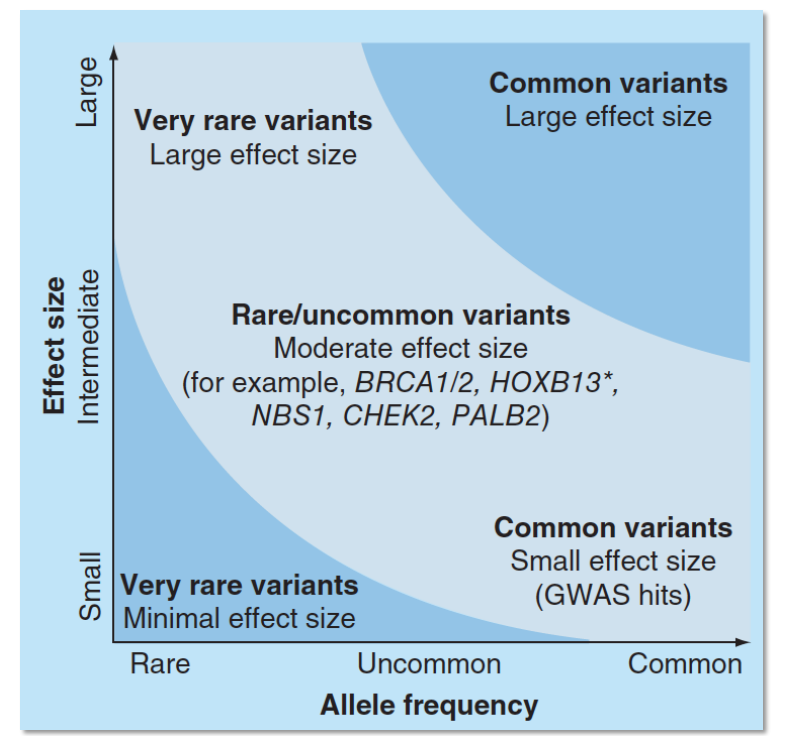
\includegraphics[width=0.5\textwidth]{relevance.png}
    \caption{R. Eeles, Future Sci. OA (2016) 2(1), FSO87. Review on prostate cancer}
    \label{fig:relevance}
\end{figure}

\paragraph{Penetrance}
Penetrance is the proportion of individuals carrying an allele (or genotype) that also expresses the trait (or phenotype) associated with it.

\paragraph{Allele frequency}
Allele frequency is the ratio between the number of times the allele of interest is observed in a population over the total number of copies of all the alleles at that particular genetic locus in the population.
			
Recent studies have shown that genetic variance contributes to predisposition to certain deseases. 
What is also emerging is that if we are dealing with a very rare variant, if this variant is pathogenic, it haso also high penetrance.
Meaning, if the variant is pathogenic and very rare, it's very probable that all patients affected by the desease carry this mutation. This is shown in the top part of the diagram shown in figure \ref{fig:relevance}.
On the other hand, common variants could be associated to predisposition or susceptability to the deasese, but the penetrance is very low. 
In the middle on the diagram we find very well-known variants correlated to cancer. The majority of these have a moderate size effect (not everyone who has the variation develops the desease).

\subsection{Differences in Genetic Make-Up, an example}
One example of how the genetic make-up plays a role in deases is the ADME genes. 
ADME stands for \textit{Absorption, distribution, metabolism and elimination}. 
It is a set of genetic variants that are able to change ability of the organism to react to certain compounds (pharmacokinetic variability),influencing the patients’ treatment response.
Both common and rare variants are involved.
A therapeutic approach that considers these variations could be very useful in precision medicine.

Somatic variance: not acquired from parents. SNV and SNP are basically the same thing, but SNV are restricted to a certain population of cells, while SNP are genetically encoded in all cells of the organism. Other types of somatic variance are rearrangemets (gene translocation, chromosome breakage, chromotripsy), somatic copy number changes are equivalt to copy number variance but somatic (SCNA). 

\subsection{Acquired DNA aberrations}
Variants that are not inherited from parents and are not transmitted to offspring are called \textbf{somatic variants}. 
They are usually caused by DNA aberrations.
DNA aberrations happen in diseased or aged cells and are the key to cancer genomics.
They can be 
\begin{itemize}
\item  Single nucleotide variants (or SNV or point mutation). SNV and SNP are basically the same thing, but SNV are restricted to a certain population of cells, while SNP are genetically encoded in all cells of the organism.
\item Indels or deletions
\item Rearrangements
\item Somatic copy number aberrations or SCNA
\end{itemize}

		\subsubsection{Types of acquired DNA aberrations} \label{subsec:aberrations}
		

			\paragraph{Translocation}
			Translocation happens when a sequence is moved from one genetic locus to another.
			It can be a balanced translocation, meaning that the overall quantity of DNA is maintained (two sequences exchange locus), or unbalanced, where only one sequence move (insertion) 

			\paragraph{Inversion}
			Inversion happens when a sequence inverts its orientation. It involves only one 		chromosome.
			Importantly, in the sequence of the inversion nothing changes, the change will be detected only at the head and tail of the inversion.
Copy number changes (DNA quantity): duplication and dletion. COuld involve one or more chromosomes

			\paragraph{Copy number changes}
			It refers to a change in the quantity of DNA. 
			In duplication a sequence doubles its copy number.
			In deletion a sequence is lost.

			\paragraph{Chromoplexy}
			From the Greek \textit{pleko}, meaning to weave, or to braid.
A class of complex somatic DNA rearrangements whereby abundant DNA deletions
and intra- and inter-chromosomal translocations that have originated in an
interdependent way occur within a single cell cycle. 

			\paragraph{Chromothripsis}
			(From the Greek \textit{thripsis}, meaning shattering into pieces).
A clustered chromosomal rearrangement in confined genomic regions that results
from a single catastrophic event, usually limited to one chromosome. 
			\paragraph{Kataegis}
			 (From the Greek kataigis, meaning thunder).
A phenomenon that is characterized by large clusters of mutations (hypermutation) in
the genome of cancer cells. An APOBEC family enzyme might be responsible for the
kataegis process.

\footnote{See  Khurana E et al, NATURE REVIEWS | GENETICS, 2016 }


\section{Experimental techniques to detect variants/aberrations}
\subsection{Cariotyping}
Basically all the aberrations described in \ref{subsec:aberrations} were discovered in the last 10-15 years because there's the need of NGS. 
Cariotyping indeed is not enough! 
Sequence specific variants, breakpoints, etc. could not be detected until NGS. 

\section{Sequence capture for cancer genomics}
In the paper \footnote{Meyerson et al., Nature Reviews Genetics 2010} it is described a typical sequence capture for cancer genomics. 
One of the main realizations is that the test reference genome is the normal (non-cancer) DNA. 
Intuitively, we align both cancer and normal DNA so that we can detect if an aberration is cancer specific or it is present also in the normal DNA. 
The \textbf{match normal} is used to distinguish SNV from rare SNPs, but also copy number variation. 
Baits are nowadays used in the sequencing step, in order to sequence only the exome (usually, money issue). 
Another concept is the need to sequence \textit{deeply}, to find subclonal events that give the cancer maybe some fitness (escaping immune system), but also because if the sample comes from the tissue, there are both cancer and some healthy cells and we need to able to distinguish them.
A more in depth discussion is provided in *paper*.

\subsection{Single End (SE) and Paired End (PE) reads}
Paired end useful especially for detecting structural variance. Massive information of relative position of a molecule wrt the reference gneome.

\begin{figure}[htbp!]
    \centering
    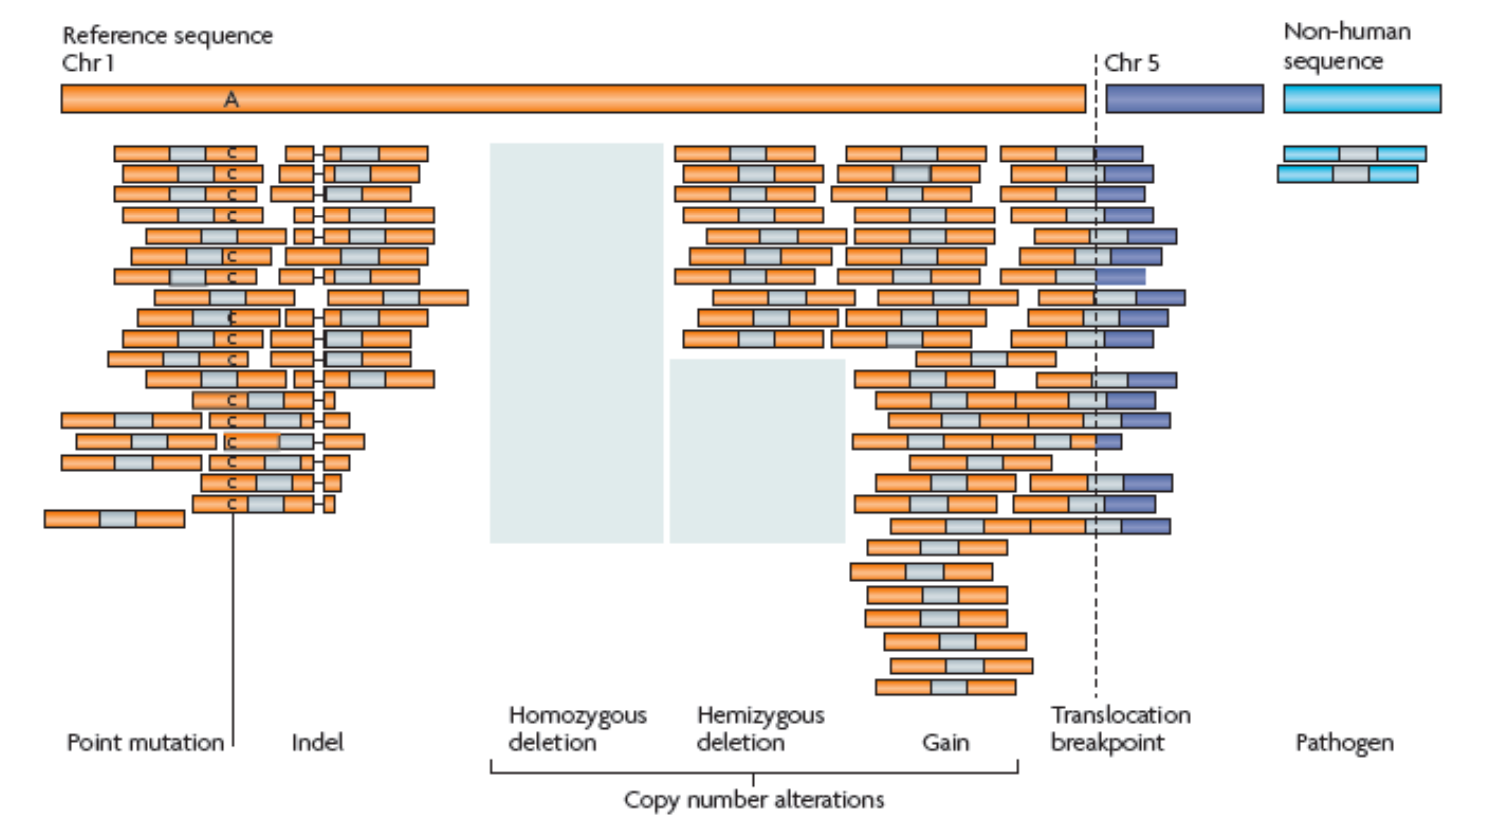
\includegraphics[width=0.7\textwidth]{igv.png}
    \caption{\textit{Advances in understanding cancer genomes through second-generation sequencing}, Meyerson et al., Nature Reviews Genetics 2010}
    \label{fig:igv}
\end{figure}

Figure \ref{fig:igv} gives a nice graphical overview of genomic aberrations detectable by NGS, especially using PE sequencing. 
Important to notice is that performing PE sequencing is like having double the coverage. 
Both for homozygous and hemizygous deletions and insertions the single most important thing we need to care about is to have enough coverage on the whole experiment to perform significative downstream analysis. 
An important thing to notice in \ref{fig:igv} is the translocation breakpoint: without PE we would not be able to detect the translocation event. 

 
















   \graphicspath{{chapters/02/}}
\chapter{Coverage}
\section{Local Coverage and Allelic Fraction}
Two key concepts needed when perfoming genomics analysis are the \textbf{local coverage} and \textbf{allelic fraction}.

	\paragraph*{Local coverage (cov)}
		The local coverage (cov) at position (base) $i$ is the number of reads that span $p_i$.
	\paragraph*{Allelic fraction (AF)}
		The allelic fraction (AF) at position $i$ is the proportion of reads that supports 			the reference base in $p_i$, and viceversa. 

The Lander-Waterman equation to compute NGS coverage is:
\begin{equation}
C = \frac{L * N}{G}
\end{equation}
Where G is the coverage, G is the haploid human genome length, L the read length and N the number of mapped reads.

\subsection{Mapping in NGS}
The number of mapped reads is always lower than expected. Errors, or major translocation will impair a good mapping of the reads. \\
There's a difference between physical and sequence coverage. Physical coverage is always higher, and it changes based on which protocol (PE or SE) is chosen for the assay.
To put it simply, when calculating the sequence coverage we only take into account the actual ends, while when calculating the physical coverage we also account for the consequence part of the PE protocol. In figure \ref{fig:seq_phys} a  shcematic representation of this problem is displayed.
\begin{figure}[htbp!]
    \centering
    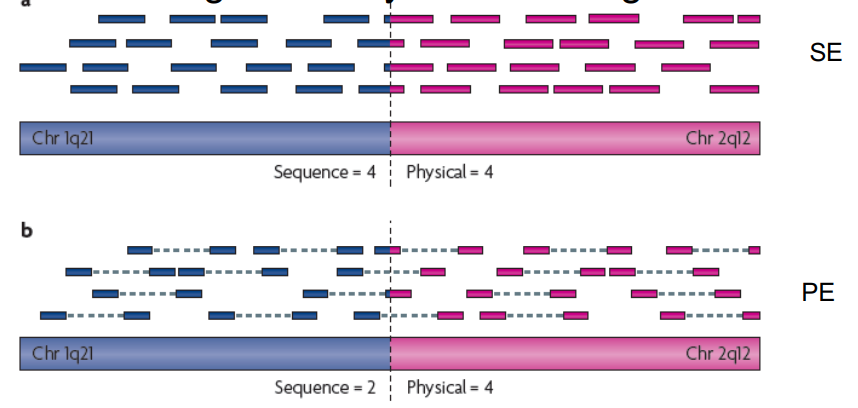
\includegraphics[width=0.5\textwidth]{seq_phys.png}
    \caption{Schematic difference between sequence (on the left) and physical coverage (on the right). From Meyerson et al., Nature Reviews Genetics 2010}
    \label{fig:seq_phys}
\end{figure}

Formal definitions of sequence and physical coverage are:

\paragraph*{Sequence coverage:}
	Sequence coverage is the amount of oversampling (how many times a base is sequenced); to detect nucleotide alterations with high sensitivity, the 3 billion bases of the human genome have typically been ‘covered’ with at least 30-fold (30X) on average, meaning 90 billion bases of sequence data per sample. 
	\paragraph*{Physical coverage:}
		the expected distance between the paired reads is used to uniquely place the reads on the genome; unexpected read pairs are used to detect structural anomalies.
		
		

\section{Tuning the intended coverage of a NGS assay}
In some experiments setups there's the need to carefully control the amount of intended coverage. \\
If we are looking for SNPs only, which by definition are present in all of the cells, we only need enough redundancy (local coverage) to detect them and distinguish the reference base and the alternative base (in case of an heterozygous SNP we will ideally find half of the reads supporting the reference and half supporting the alternatice). Indeed for SNPs we do not need more than 10-15 X coverage. 
\\
However, if the sample comes from a tumor or hematopoietic events, we need to look for subclonal events. Subclonal events are not harbored by all of the cells but only by a fraction of them. If we expect 1/4 of the cells harboring the mutation, we need to increase the coverage. \\
The same reasoning goes for any monozygous mutation and any low abundant events, and for  transcripts expressed at very low level (RNA-seq) and weak binding in ChIP-Seq. 

\subsection{Example on the importance of coverage}
Here are represented 10 genes relevant for cancer. Each bar represents the average local coverage at 30 bp.
\begin{figure}[htbp!]
    \centering
    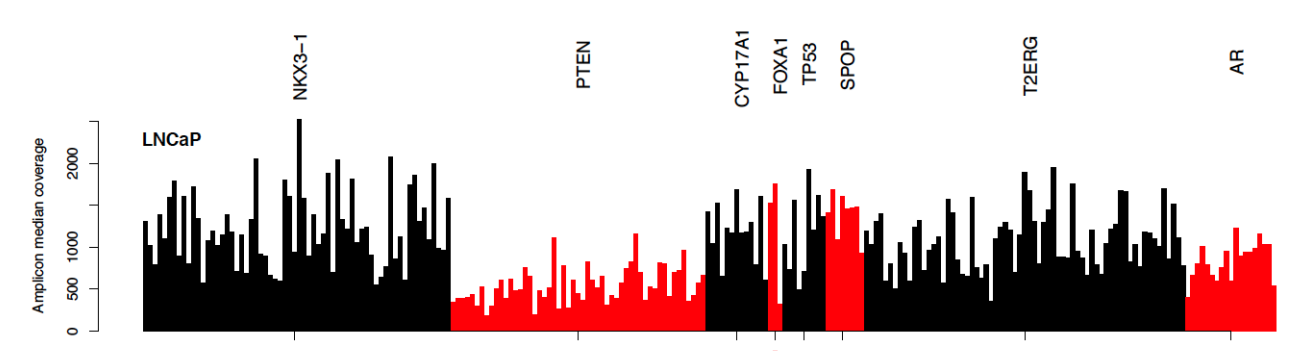
\includegraphics[width=0.5\textwidth]{local_coverage.png}
    \caption{Example of local coverage. On the x axis genomic location (on top e ery gene) and the bars is the number of amplicons. }
    \label{fig:local}
\end{figure}

In figure \ref{fig:local} a barplot can be observed, representing the local coverage (y axis) in the gene locations (x axis). The \textit{cov} is on average about 600x and it's "wavy", not evenly distributed (very typical). However, if one would do an average of the coverage for each gene, they would discover that one gene is abundantly underrepresented: PTEN.\\
What's happening on PTEN base on plot \ref{fig:local}? Probably, the most accurate guess is a deletion. But of which kind? For sure not a homozygous deletion, since we would not be able to see any signal in the plot. From this data however we cannot say whether this is a monoallelic or biallelic deletion. \\
Note that this (and the following \ref{fig:local2}) plot is the actual way sequencing data is shown, while the figure presented in \ref{SE_PE} was a schematic representation. 

\begin{figure}[htbp!]
    \centering
    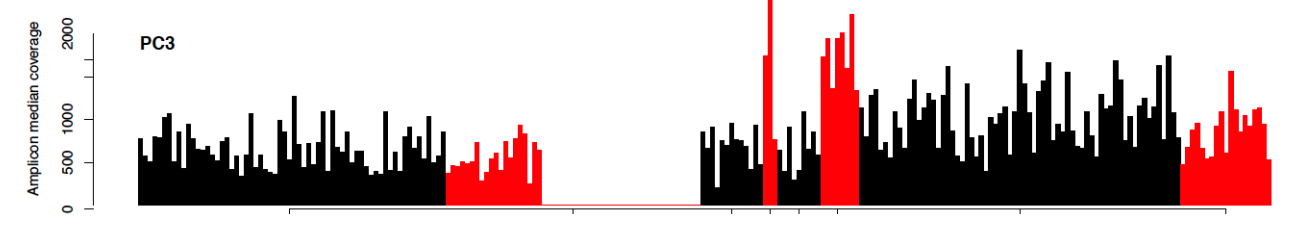
\includegraphics[width=0.5\textwidth]{local_coverage1.png}
    \caption{Example 2 of local coverage. The  cell line is different (PC3 instead of LNCaP). }
    \label{fig:local1}
\end{figure}

However, in the plot \ref{fig:local1}, from a different cell line, we can see a clear monoallelic deletion and a partial biallelic deletion of PTEN.\\

\begin{figure}[htbp!]
    \centering
    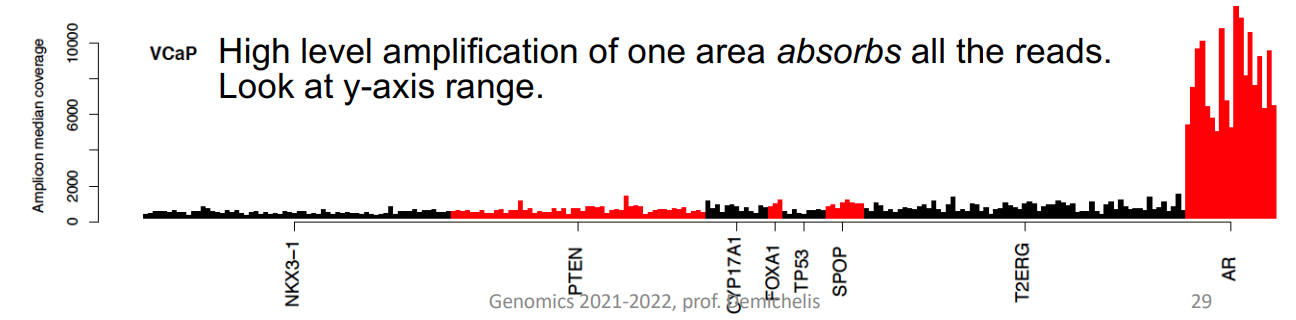
\includegraphics[width=0.5\textwidth]{local_coverage2.png}
    \caption{Example 3 of local coverage. The  cell line is different (VCaP). The massive amplification of the AR region is typicall in advanced prostate cancer.}
    \label{fig:local2}
\end{figure}

In figure \ref{fig:local2} we can see a massive amplification of the antigen receptor. Probably it was a mistake in the assay: amplification on the AR does not allow the analysis/discovery of other copy number variations because all of the reads will go to the AR site. \\
These were amplicon-based approaches. 
With NGS instead, It is easy to increase the experimental coverage (i.e. the sequence depth) at later point in time. 
Provided our original sample/library is still available, we can perform another run of sequencing and then combine the output from different runs. 
Note that this isn’t possible with array-based technologies.\\
However, there are some limiting factors of NGS DNA-seq experiments. 
Problems with repeated regions, but also not knowing the linearity of the genome. 
If the sequencing is done with longer reads we could tackle the problem by having longer molecules to work with, but there are more errors in the reads. 

\subsection{Databases}
Two very known databases for NGS analysis are:
\begin{itemize}
\item \textbf{Genome Reference Consortium}: assemble a reference genome reflecting the most common sequences in population at each position while tracking information on polymorphisms. 
\item \textbf{USCS Genome Browser}: select a reference genome and query all known features.
\end{itemize}

\section{Interpreting Pair Orientations}
We will now look at some aberrations' discoveries performed using IGV.\\
In IGV, each vertical bar corresponds to a read. 
If there is a colored sign, there is a polymorphism or difference with respect to a reference. 
The bowser also gives info about the quality of the read and bases (and others from the BAM file).\\
While using a paired-end protocol, we can study inversions, duplications and translocations. A useful legend to navigate the subsequent example is reported in the list below.
\begin{itemize}
\item \textbf{LR} ($\rightarrow \, \, \, \leftarrow$): Illumina (convention), the reads are left and right of the unsequenced part of the sequenced DNA fragment when aligned back to the reference genome;
\item \textbf{LL}, \textbf{RR}: implies inversion in sequenced DNA with respect to reference ;
\item \textbf{RL}: implies duplication or translocation with respect to reference;

\end{itemize}

\subsection{Inversion}
To detect major aberration, like inversions, we need reads that span the breakpoint (either long reads, or, better, PE reads). \\
What's happening exactly at the breakpoint in figure \ref{fig:inversion}? What's the coverage when looking at the data?  When we map them on the reference, we see that the direction is LL and RR, meaning that there is an inversion.
%The sequence that we have in the molecule does not exist there and therefore that sequence doe not exist in two copies in the molecule. 
We can also spot a drop in the local coverage.  
In the target molecule, either it does not exist or exist only in one allele and not the other one. \\
When interpreting structural variance, we need not to care only about end-orientation, but also coverage at the exact break point, which is due to the fact that the inverted breakpoint sequence does not exist in the reference genome.


\begin{figure}[htbp!]
    \centering
    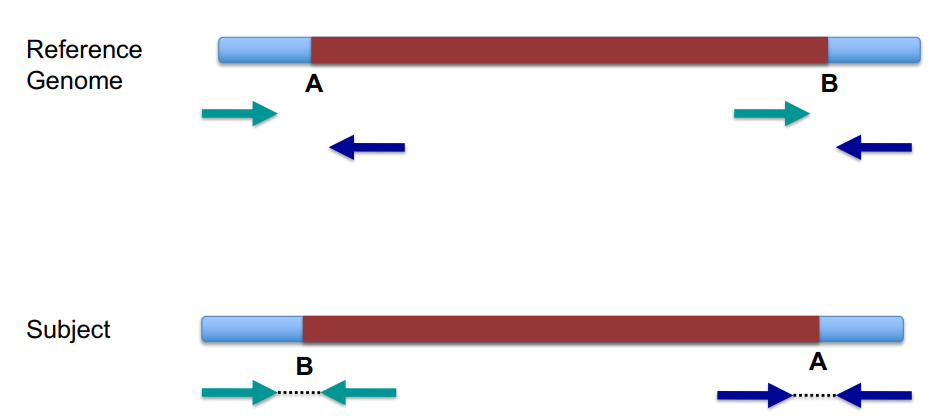
\includegraphics[width=0.5\textwidth]{inversion.png}
    \caption{Inversion disocvering exploiting PE reads.}
    \label{fig:inversion}
\end{figure}


\subsection{Tandem duplication}
Notice how in the tandem duplication (figure \ref{fig:tandem}) all the reads that do not cover the junction point align perfectly to the reference.
The coverage will be 3/2 of the expected value, proportional to the extra copy. B junction and A junction will not have modifications. If we had a read mapping BA, we would observe a partial alignment at B on the reference.
We observe no drop of coverage because the sequences also exist in the reference. \\

\begin{figure}[htbp!]
    \centering
    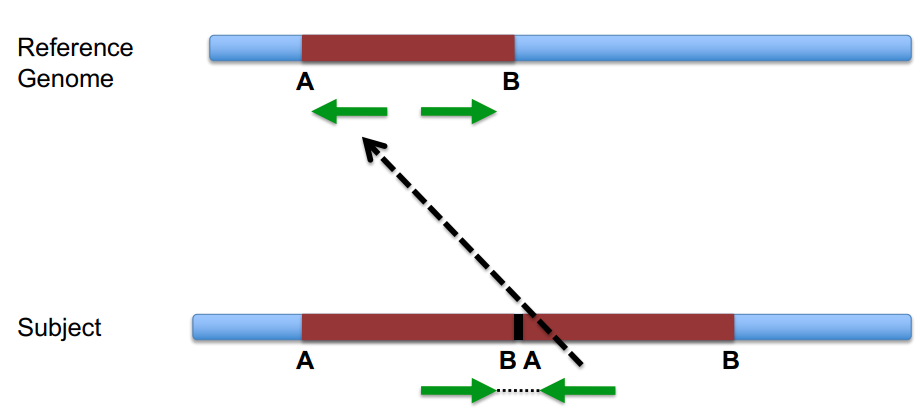
\includegraphics[width=0.5\textwidth]{tandem.png}
    \caption{Tandem duplication discovering exploiting PE reads.}
    \label{fig:tandem}
\end{figure}

\subsection{Inverted duplication}
For the inverted duplication, in figure \ref{fig:inverted, we expect double coverage in the duplicated site in the reference genome. \\
Both A and B on the first segment on the subject are LR oriented, and the same occurs in the reference genome. 
When we add the second fragment the same holds, but direction will be LL and RR and the insert size will be significantly longer. In particular, we can notice that we have an overlapping of left and right reads on the reference. Furthermore, the coverage depth will highly increase due to the presence of multiple reads on the reference genome.

\begin{figure}[htbp!]
    \centering
    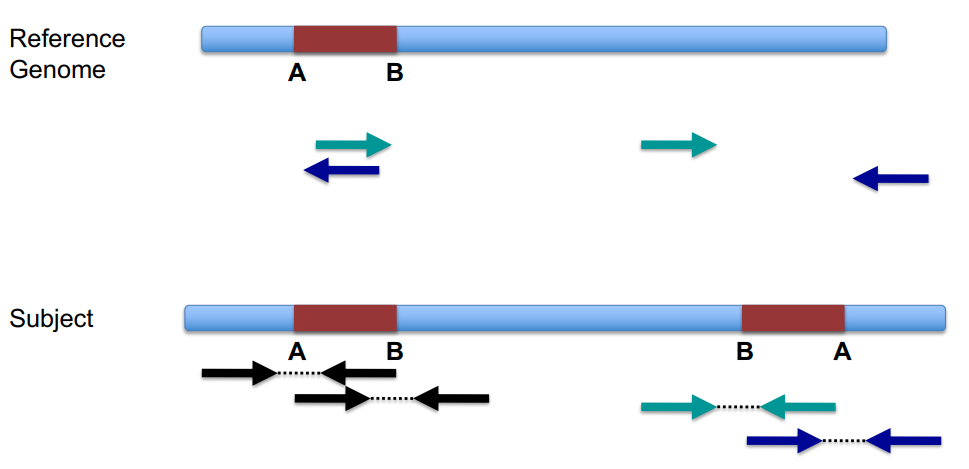
\includegraphics[width=0.5\textwidth]{inverted.png}
    \caption{Inverted duplication discovering exploiting PE reads.}
    \label{fig:inverted}
\end{figure}

What if we have a deletion? How can you guess the size of it? We can look at the coverage or observed distance between the reads, which gives clean indication of the size of the deletion. For tiny deletions, smaller than the length of the read, we use the sequence within the reads and in this way discovering indels.  

\section{Summary}
Summarizing, the elements to consider are:
 \begin{itemize}
 \item Pair ends relative orientation;
 \item Insert size length; 
\item Coverage within the aberrant region; 
\item Coverage outside of the aberrant region (flanking genomic segments); 
\item Coverage at the breakpoints. 
 \end{itemize}





 

















    \graphicspath{{chapters/03/}}

\chapter{Genetic Fingerprinting}
Genetic fingerprinting is a technique used to identify some characteristics of a genome (a pattern of variable elements), like SNPs or minisatellites, in order to uniquely characterize a genome.\\
Genetic fingerprinting can be used to compare a genome with a reference sample or to compare different genomes between each other, in order to determine their diversity or analogy. 

DNA fingerprinting is applied in different fields:

\begin{itemize}
	\item In forensics, for identification purposes;
	\item In lineage related tests, for cells or humans. Eg. pternity test, hereditary tests.
	\item For the certification of the origin of cells used in the laboratory, to make sure that the cells are the right ones and that there are no major genetic drifts. Needed when using certain cell lines, for publishing purposes.
\end{itemize}


\subsection{Variants used for genetic testing}
There are different variants that can be used for genetic fingerprinting, such as Single Nucleotide Polymorphisms (SNPs) or inherited Copy Number Variations (CNVs).
Remember: SNPs are substitutions of a single nucleotide at a specific position in the genome, whereas copy number variation is a phenomenon in which sections of the genome are repeated and the number of repeats in the genome varies between individuals.\\
Basically everything that is inherited and that is a polymorphism can be used in genetic testing, however some variants are more amenable than others.
SNPs are the most \textit{amenable} ones, since they are simple, abundant in the genome and easy to detect in sequencing data at any coverage depth. For these reasons, in this chapter we will focus on the development of SNP-based genetic tests.

\section{SNPs features}

\subsection{Hardy-Weinberg equilibrium and Minor Allele frequency}

One property of SNPs which has to be taken into account when using them for genetic testing is the \textbf{Hardy-Weinberg equilibrium}. 
In population genetics, the Hardy-Weinberg equilibrium states that allele and genotype frequencies in a population will remain constant from generation to generation under neutral selection, so in the absence of other evolutionary influences, like genetic drift, mate choice, sexual selection, mutation and so on.

In the simplest case of a single locus with two alleles denoted \emph{A} and \emph{a} with frequencies f (A) = p and f (a) = q, respectively, the expected genotype frequencies under random mating are f(AA) = $p^{2}$ for the AA homozygotes, f(aa) = $q^{2}$ for the aa homozygotes, and f(Aa) = 2pq for the heterozygotes. In the absence of selection, allele frequencies p and q are constant between generations, so equilibrium is reached. The general equation that the allele frequencies need to fit in to be considered in equilibrium is:

\begin{equation}
( P + Q )^2 = 1 \, , \, P^2 + 2PQ + Q^2 = 1 .
\end{equation}

SNPs that respect this equilibrium are also the most studied, thus more informative. 

\subsection{Minor Allele Frequency}
When performing genetic fingerprinting, the aim is to maximize the probability to have different genotypes in unrelated individuals. \\
For this reason, the more advantageous SNPs will be the ones in which the allelic frequency of the variants is the highest possible. Highest variability in the population allows to distinguish better more individuals. 
\\
Number-wise, a frequency of $\frac{1}{3}$ for each SNP would maximize the variability, but those SNPs wouldn't be in HW equilibrium and we might have missed calls. \\
Therefore, the optimal SNPs to detect individuals’ differences and similarities are those with genotype frequencies: $P_{AA}$ = 0.25, $P_{BB}$ = 0.25, $P_{AB}$ = 0.5. 50\% of individuals for that SNP will have a heterozygus genotype, 25\% a homozygus genotype for the reference allele, 25\% for the alternative allele.
\\
This is equivalent to say that best SNPs will be the ones with \textbf{MAF} = 0.5. Minor allele frequency (MAF) is the frequency at which the second most common allele occurs in a given population.

\subsection{Projects regarding SNPs}
Some useful projects developed over the years are:
\begin{itemize}
	\item \textbf{dbSNPs}: it is a database of small scale nucleotide variants. The database includes both common and rare singl ebase nucleotide variation (SNV), short ($\leq$ 50bp) deletion/insertion polymorphisms, and other classes of small genetic variations.
	\url{https://www.ncbi.nlm.nih.gov/snp/}
	
	\item \textbf{HapMap3}: is the third phase of the HapMap project whose aim is to develop a haplotype map of the human genome to describe the common patterns of human genetic variation in order to allows researchers to find genes and genetic variations that affect health, disease and individual responses to medications and environmental factors. The HapMap is a catalog of common genetic variants that occur in human beings. It describes what these variants are, where they occur in our DNA, and how they are distributed among people within populations and among populations in different parts of the world.
	\url{https://www.sanger.ac.uk/resources/downloads/human/hapmap3.html}
\end{itemize}

\subsection{Haplotype Blocks}

Another important feature to consider for SNPs selection are \textbf{Haplotype blocks}. Haplotype blocks are blocks along the genome that tend to be inherited as segments (no recombination inside a haplotype block). In these sizable regions there is little evidence for historical recombination and only a few common haplotypes are observed. \\

So for example, if there are 10 SNPs in a block of 1 MB, the genotype of one specific SNP in that block gives an indication the genotype of the other SNPs in the same block, since they are inherited together. 
Hence, if there is a haplotype block, there is no point in sequencing all SNPs in that block, it is sufficient to select some specific SNPs. Also, when running a fingerprint assay, there is no point in using all SNPs in a haplotype block since they won't bring additional information independently.\\

SNPs in the same HB are said to be in \textbf{Linkage Disequilibrium} (LD). Linkage disequilibrium measures the non-random associations between alleles or polymorphisms at different loci. A higher LD indicates a SNPs with a stronger tendency to co-segregate.
Haplotype Blocks are therefore commonly represented with \emph{linkage disequilibrium plots} \ref{fig:linkage}. In these plots, SNPs are represented in a way that does not respect the genomic distance, but the order along the genome (position of each SNP relative the others). 

% aggiungere LD plot - slide 7
\begin{figure}[H]
	\centering
	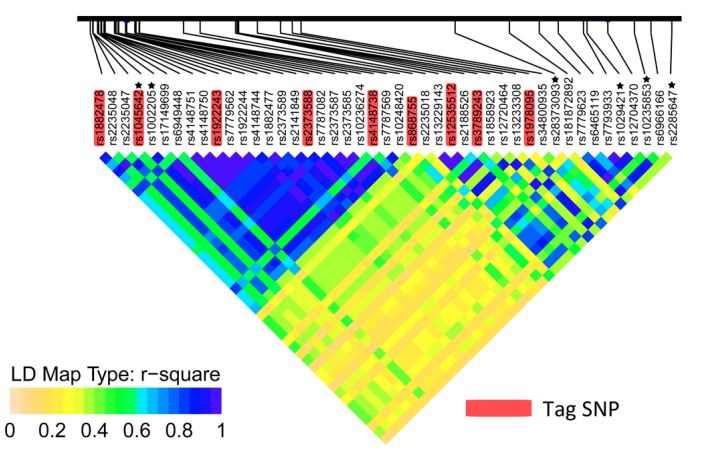
\includegraphics[width=0.7\textwidth]{linkage.png}
	\caption{\label{fig:linkage}LD plot of SNPs with top-ranked bayes factors in CHB (Han Chinese in Beijing) of 1000 Genome Phase I. The colors indicate the
strength of pairwise LD according to r2 metrics. The SNPs marked with asterisks represent independent strong associations. Tag SNPs are here shadowed in pink.}
\end{figure}

The colors indicate the strength of pairwise linkage disequilibrium (LD) according to r2 metrics. In fact, not all of the SNPs are informative to distinguish between individuals. \\
In \ref{fig:linkage} \textbf{Tag SNPs} are shadowed in pink. A Tag SNP is representative of a region with high linkage disequilibrium and represents a group of SNPs (called haplotype).

\subsection{Other SNPs features} 
Other SNP features to take into consideration when analyzing:
\begin{itemize}
	\item Choose SNPs that are in areas that are not likely to undergo somatic aberrations. So exclude chromosomal locations which undergo frequent somatic aberrations, e.g. areas commonly deleted in tumor will produce LOH but probably also no calls, since there is no DNA. 
	\item Choose SNPs equally represented/spread all around the genome (not in specific chromosome regions).
	\item Select autosomal only SNPs (not on chromosome X).
	\item Select SNPs in exons. If we were to run a targeted assay, this would cover more exons instead of introns. It will also be more probable to have signal from a non-DNA assay, for example if calling a genotype from RNA sequencing data (even though it is not always done).
	\item Exclude/include disease or drug response associated loci. 
	\item Include/exclude loci with significantly different MAF in different ethnicity. If we include them we can also have a lineage type of tests in the same assay. 
\end{itemize}


\subsection{Number of SNPs to select} 

If we want to build a test to run genetic fingerprinting using SNPs, how many polymorphic loci (SNPs) should be tested?\\
We want to make sure that the measure of the test will be able to differentiate unrelated individuals. 
But we must also remember that many variables must be taken into account, possible mismatches in particular. Those can be due to the sequencing process itself (experimental mismatches) but also to changes due to somatic events (biological mismatches). All these events can be used in the test with a different weight, based on how likely they are. 


\subsubsection{Experimental mismatches : Genotype call error rate}

During sequencing, each machine will produce some errors, resulting in some loci for which no data will be available. If those loci include some SNPs of interest, then no call will be associated to that SNP. 
Experimental mismatches are related to the error rate of the technology used, they are platform dependent. 

\paragraph*{Some examples:}

\begin{figure}[H]
	\centering
	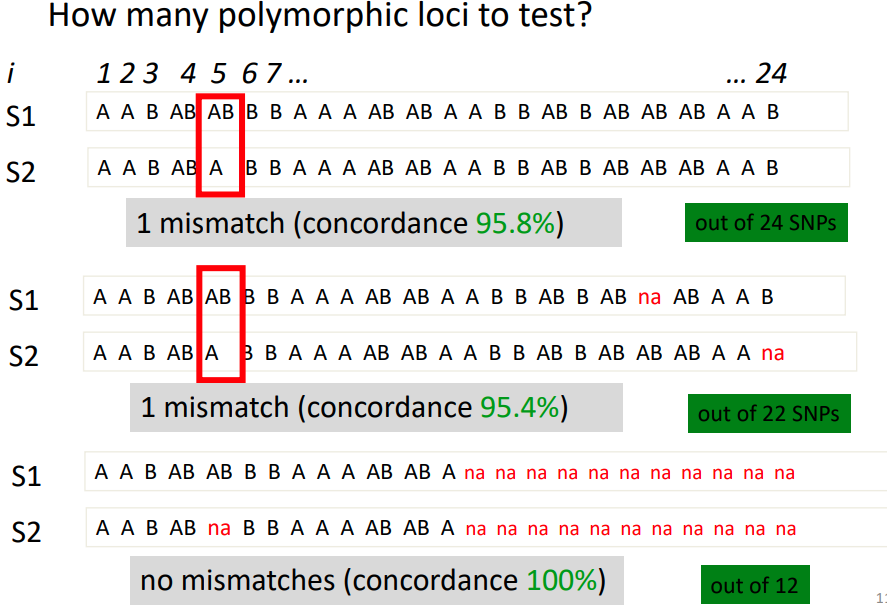
\includegraphics[width=0.7\textwidth]{SNP.PNG}
	\caption{\label{fig:SNP}}
\end{figure}

In each example in figure \ref{fig:SNP} there are two samples with the same number of potential SNPs: 24. To determine the difference/similarity of the two samples we can look at the genotype for each position and count mismatches.

Legend: \\
\begin{itemize}
\item 'A' stands for 'AA' (e.g. homozygus genotype for the reference allele); often referred to as Aa.
\item 'B' stands for 'BB' (e.g. homozygus genotype for the alternative allele); often referred to as Bb.
\item 'AB' stands for heterozygus.
\end{itemize}

Now, analyzing the three cases in figure \ref{fig:SNP}:
\begin{itemize}
	\item First Example: over the 24 loci, there is only one mismatch. This translates to a level of concordance of 95.8\%. Those 2 individuals are highly related or DNA comes from the same samples.    
	\item Second example: there is only one mismatch but there are some 'na', indicating that for some positions we don't have a call (not available data). Therefore, in this case the concordance is measured out of 22 SNPs and is equal 95.4\%. 
	\item Third example: here a lot of 'nas' are present, leading to have only 12 SNPs available. This brings to a concordance of 100\%. 
\end{itemize}

Different examples produced different levels of concordance. What do we trust the most?
\\
The first set of SNPs is the one that we trust the most, because it has the higher number of available SNPs. Wider number of SNPs provides the most reliable information. 

\subsubsection{Biological mismatches}
In the context of disease samples and tumors, many somatic events can happen, like deletions, gains of copies, homozygus deletions, ecc. Some common ones are:
\begin{itemize}
	\item  \textbf{Loss Of Heterozygosity (LOH)}:  event that results in loss one parental copy of a region which results in the genome having just one copy of that region. If that region contained a heterozygus locus (e.g. SNP), there will be loss of heterozygosity.
	
	\begin{equation}
	\textit{probability of AB $\rightarrow$ A: }P(AB,A) = P(AB) * P(A | AB)
	\end{equation}	  
	
	\item Gain Of Heterozygosity (GOH): due to a mutation in a site often polimorphic through inheritance. These are pretty rare.
	
	\begin{equation}
	\textit{probability of A $\rightarrow$ AB: }P(A,AB) = P(A) * P(AB | A)
	\end{equation}	
	
	\item Double Mutation (DM): very rare.  
	
	
	\begin{equation}
	P(A,B) = P(A) * P(B | A)
	\end{equation}	
\end{itemize}

\bigskip
Biological mismatches can be properly modeled in our assay. We can, in a data driven way, assess the error rate for the genotyping for some specific SNPs or run tests. We can also think in terms of SNP-specific or tissue-specific probabilities.
\\
The joint probability of two events $E1$ and $E2$, $P(E1,E2)$ or $P(E1 AND E2)$ is $P(E1,E2) = P(E1) * P(E2|E1)$ and $P(E2|E1)$ is called the conditional probability of $E2$ given $E1$. 
\\

The main point is that all mismatches must be taken into consideration. 
For this, all implemented tests use more than the minimal number of SNPs that allow to identify individuals. 

\section{Genetic Distance}
Having defined the number of SNPs to use, with maximum MAF and other amenable characteristics, the genetic test should provide a measure of some sort, which will be the output metric, associated with a probability of the measure to be correct. 
\\
As a simple measure, we can count the number of loci where two samples show different genotype and normalize on the total number of queried loci, defining a certain level of discordance (or concordance). The output value will be the 'genetic distance' between the two samples given the selected loci. The distance is proportional to the number of discordant calls.
\\
In figure \ref{fig:Distance} we can see an example of a typical graph used to measure the genetic distance using SNP-based genetic testing. We have 4 samples with a set of 5 SNPs for each one. The distance is measured among all possible pairs, whose indexes are reported on the x-axis. 

\begin{figure}[H]
	\centering
	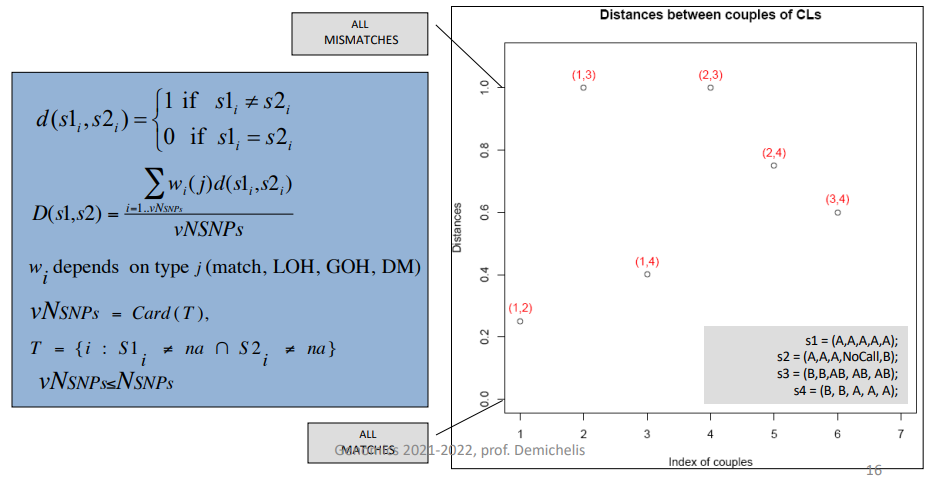
\includegraphics[width=0.7\textwidth]{loci.PNG}
	\caption{\label{fig:Distance}Genetic Distance graph with 4 samples. On the y axis we have the genotype distance, allegedly from 0 to 1. On the x-axis we have the index of all possible pairs in the dataset.}
\end{figure}


\begin{itemize}
	\item s1 and s2 have 3 A in common, one locus has no call and another one produces a mismatch. 1 mismatch out of 4 produce a distance of 0.25.
	\item samples s1 and s2 have 5 mismatches out of 5, so a distance (or discordance) of 1. 
\end{itemize}


If we put that into an equation will have that: for each position i (SNP) between sample 1 and 2 we can have 1 if the genotype is different, 0 if they are identical. Then we determine the distance D by summing up the different scores obtained for each SNP. We can associate different weights $w_i$ to different mismatches or we can put all equal to one. Then we divide by the total number of SNPs for which we have available calls, vNSNPs, which will be lower or equal to the total number of SNPs, NSNPs. 

\begin{figure}[H]
	\centering
	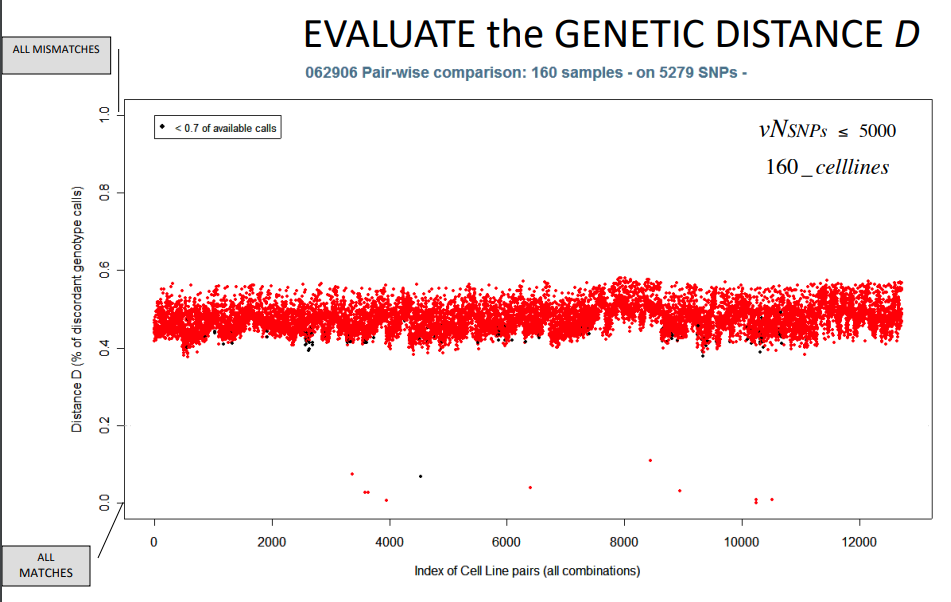
\includegraphics[width=0.7\textwidth]{loci2.PNG}
	\caption{\label{fig:Distance2}Genetic Distance graph with 160 samples}
\end{figure}

This other example at figure \ref{fig:Distance2} shows the distance, measured by genetic fingerprinting, of a collection of 160 samples of cell lines. 
\\
The number of possible pairs corresponds to: $160 * 159 / 2$ (number found in the x-axis). 
\\
By applying this measure to a larger collection of samples like this one, with many SNPs, we expect to find an \textbf{average distance} among all possible pairs that very unlikely will be close to 1. 
The MAF of the SNPs is 0.5 but it will never happen that, with a high number of SNPs, the discordance will be 1. We will have an average distance that in this case around 0.5, since by chance we all share some genotypes on a large number of SNPs. 
\\
Here we find certain pairs with a very low distance, sometimes almost equal to zero (dots at the bottom). This is a surprising result because it shows that those pairs, which were suppose to be different cell lines, were actually not different cell lines (only less than 70\% of SNPs have available calls). 

% immagine slide 19
\begin{figure}[H]
	\centering
	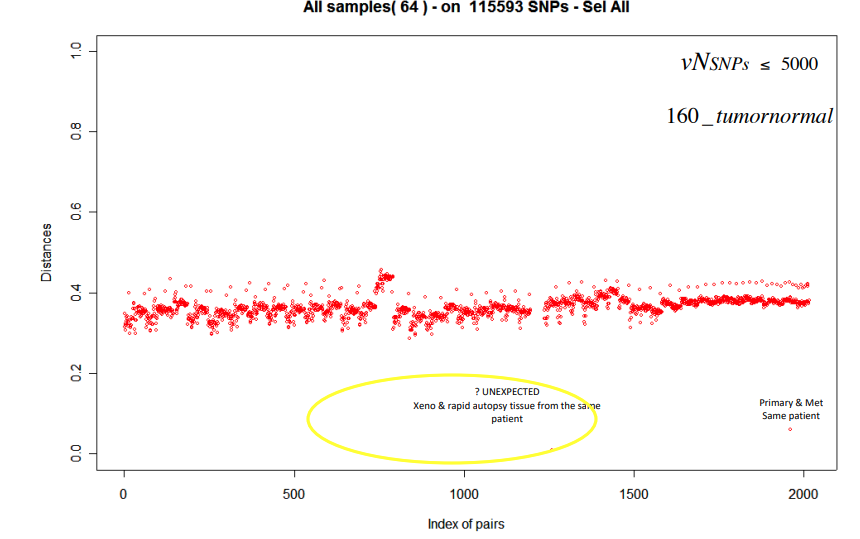
\includegraphics[width=0.7\textwidth]{loci3.PNG}
	\caption{\label{fig:Distance3}Genetic Distance graph with tumor samples}
\end{figure}


In this last example at figure \ref{fig:Distance3} genetic fingerprint was performed on a collection of 160  tumor samples, with a larger SNP array (more that 100.000 SNPs).  
\\
From the analysis, two samples with very low distance were observed. One of the two samples came from a Rapid Autopsy Progam and the other one from a xenograft model. 
\\
RAP are programs for which patients at the end of their life agree to donate their tumor tissues which can be used for research. In these very complex but highly valuable programs, the material must be taken within two hours after death. Those sample are usually highly characterized but after a while the track of the patient's identity is lost. 
Here, what happened is that one man who donated tissue by this program was sequenced and for some of those metastasis models were generated and implanted into a mouse and a xenograft model was derived. Thanks to fingerprinting it was possible to determine the same origin between xenograft and patient. 
\\
The power of this technique is very high, it allows also to identify and remove things that we don't want in our study. E.g. if running a study (like a GWAS study) on a certain interesting geographic area, we will want to remove the members of the same family because that would skew the results. Genetic fingerprint can be used for this purpose.

\subsection{Some questions}

\textbf{Q1}: Would the average of unrelated samples distance increase or decrease after selection of ideal SNPs?

If we maximize the likelihood that SNPs have a different genotype among individuals and we use these to determine the measure, then the average distance of unrelated individuals will increase.

\textbf{Q2}: Is it likely to obtain a genotype distance D = 1?

We get distance 1 only if we are looking at too few viable SNPs. Whereas with a well selected pool of SNPs, and a high enough number of SNPs, it is very unlikely that the distance is equal to 1.

\subsection{Further considerations}
How does the genetic distance among different samples change when varying the number of selected SNPs used to perform the test?

% immagine slide 26
\begin{figure}[H]
	\centering
	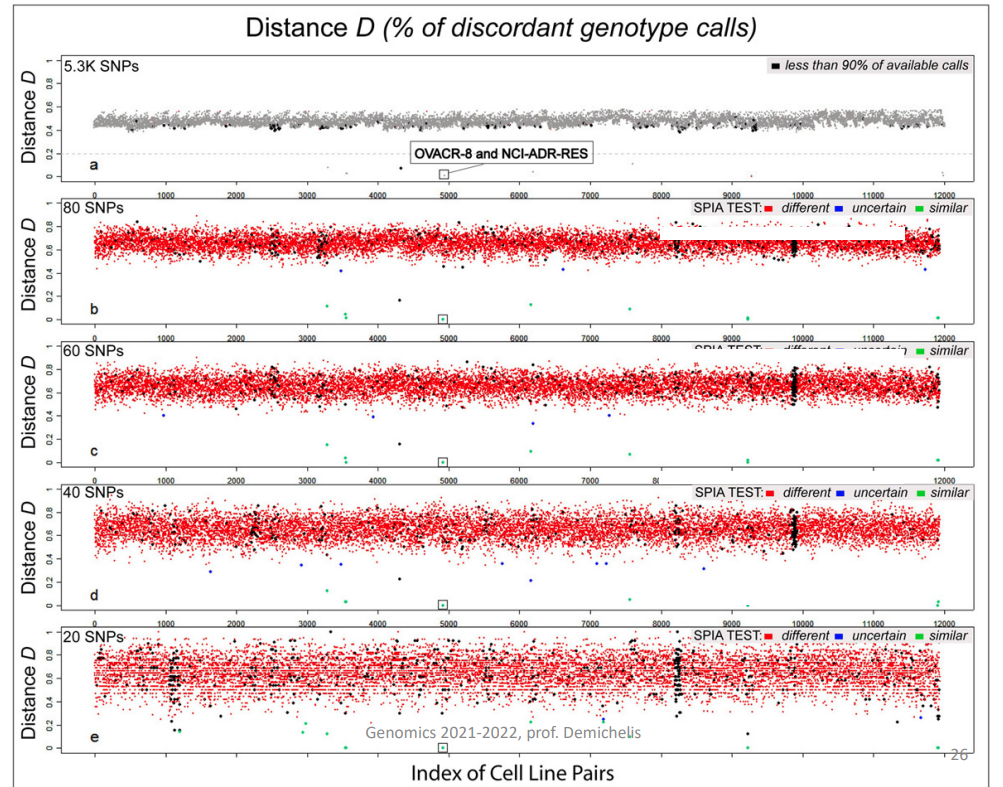
\includegraphics[width=0.7\textwidth]{selected.PNG}
	\caption{\label{fig:sel_snp}Genetic Distance graph at decreasing number of selected SNPs}
\end{figure}

The genetic distance among many samples, with an array of 5.3K SNPs, was measured, using a decreasing number of SNPs (from the initial total number of SNPs to decreasing numbers of highly selected SNPs) \ref{fig:sel_snp}. 

It is noticeable that, in the second plot where 80 SNPs matching the required characteristics were selected, the average Distance across all pairs is higher than in the previous example, in which all available SNPs were used (~0.45 vs. ~0.65). Also, the standard deviation of greater. 
Decreasing the number of SNPs to 60, then to 40 and 20 leads to have the same average distance between pairs, which settles around 0.66, but higher standard deviation.

In reality we always need enough SNPs, enough information, in order to prevent unexpected issues and to be sure that for any pairs of sample we have enough information to trust our measure. 


\section{Building a SNP-based genetic test}

Building an identity test base on SNPs is a MULTI-STEP process, consisting in: 
\begin{enumerate}
	\item Definition of a genotype/genetic distance to compare samples;
	\item Definition of SNPs requirments, based on the intention of the assay.
	\item Selection of SNPs:
	\begin{itemize}
		\item This can be done in a data-driven manner, through an iterative procedure of training and test on known sample set;
		\item Or, performing the selection based upon MAF and Hardy-Weinberg equilibrium. For example, using HapMap data.
	\end{itemize}
	\item Implementation of a probabilistic test (different, uncertain or similar)
	\item In silico validation on independent/multiple dataset.
	\item Validation on cell lines genotyped on independent platform. 
\end{enumerate}
We have already seen some of the steps needed (1, 2, 3), we now pass to the following ones.


\subsection{Implementation of a probabilistic test} 

Other important questions which we have to answer to when designing a genetic test are:
\begin{itemize}
	\item What is the threshold on the genotype distance to call two samples 'identical' ('similar') or 'different'?
	\item How confident would the call be?
    \item What is the minimum number of loci needed for a robust test?
\end{itemize}

It could be useful to have a probabilistic test to determine if the measure of the test is correct at with which level of confidence. We can use a probabilistic approach to compare observations with expectations (gold standard).
\\
Under the assumption that SNP calls at different loci are independent, we can think in terms of Binomial distribution. Each SNP can be considered as a trial, n = number of SNPs in the assay, k = number of matches, p is the probability of match and (1-p) of mismatch. Then the probability of having k matches (successes) out of N SNPs (trials) follows the binomial distribution.
\\
With n, np and np(1-p) large enough, we can use the Gaussian approximation of the Binomial distribution with $K_{mean}$ = np and sd = np(1-p). 

Using something that simple we can add a probabilistic test in our assay, defining an area of confidence given by $K_{mean} \pm m * sd$ where m is the number of standard deviations used to define the thresholds which will lead to have a smaller or wider confidence area. 

%immagine slide 33
\begin{figure}[H]
	\centering
	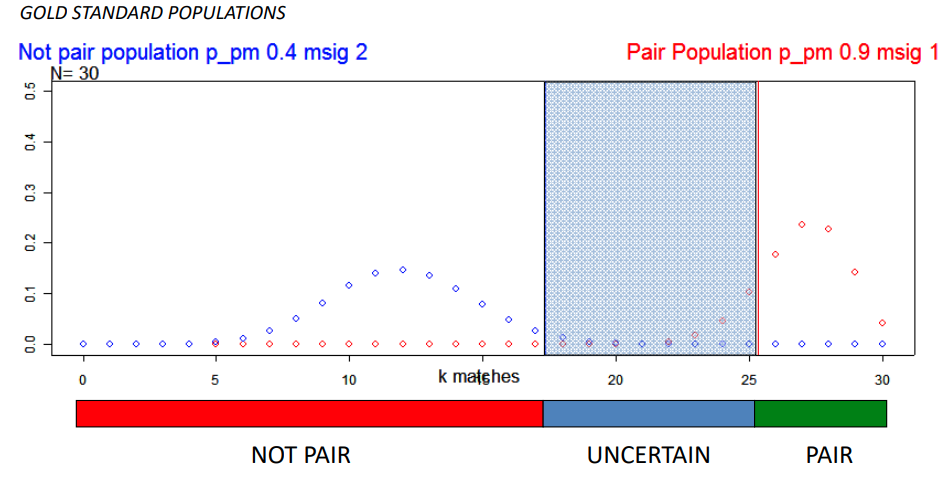
\includegraphics[width=0.7\textwidth]{double_test.PNG}
	\caption{\label{fig:prob_test}}
\end{figure}

For example: given two unrelated samples, we reason in terms of 'what is the probability of having a certain number k of matches over a total number of n SNPs, therefore a certain value of D?'. 

The probability mass function for unrelated individuals is shown in figure \ref{fig:prob_test} with a blue dotted line and indicates that there is a low probability of having both a very low and a very high number of matches. 

We can also think in the opposite term: given two related samples, what is the probability of having  matches? As represented by the red dotted line, in this case there will be a high probability of having many matches. 

Using these probabilities we can set two thresholds which will define 3 regions:
\begin{itemize}
	\item A \textbf{'not pair'} region for which the two samples will be considered as 'different'
 	\item a \textbf{'pair'} region for which the two samples will be considered as 'similar'
	\item and an \textbf{'uncertain'} region, a grey zone, for which no certain result can be produced. 
\end{itemize}

Then we can move the grey area based on what we want to be certain of and on how many SNPs we have.

By decreasing the number of SNPs, the grey zone will become more tiny, making the result more difficult to interpret. For example, a difference of only 2 matches could lead to opposite conclusions. 

By contrast, with more SNPs the area will be wider and easier to interpret. Hence using a number of SNPs greater than the minimum number is better, otherwise there will be many uncertain calls. 


\section*{Further considerations and examples}
%sistemare
In the past, before sequencing area and SNPs array area, short tandem repeats were commonly used for genetic fingerprint. They were used on gels to distinguish related and unrelated individuals, e.g., for the initial paternity test. 
\\
\textbf{Inherited copy number variants} can be used too for a fingerprinting test, but not all of them. The more amenable for this test are the loss type of CNV. In the population there will either a copy number of 2 or 1 or 0. If both parents have heterozygus pair of CNVs it will be possible that I have a homozygus deletion. If both parents have 2 copies at a site that is polimorphic in the population, we will have a genotype equal to 2 copies. 
\\
If we think about gain of CNV then it becomes messy, because when combining multiple copies and have a add up we cannot distinguish what comes from what pair, so we cannot use them to identify an individual.

\subsection{Example 1: Cell line passages}
A massive use of these genetic tests is done to assess genetic changes in in-vitro cultivation (also, in studies in tumor evolution, lineage plasticity, heterogeneity across metastasis across individuals or a single tumor).\\
Cell lines go through multiple passages in which they are used and stored. Genetic fingerprinting can be used to assess if among different passages the cells have remained the same, if they were mislabeled or if major genetic drifts happened.

% immagine slide 39 e 40
% con width = 0.4 le mette affiancate 
\begin{figure}[H]
	\centering
	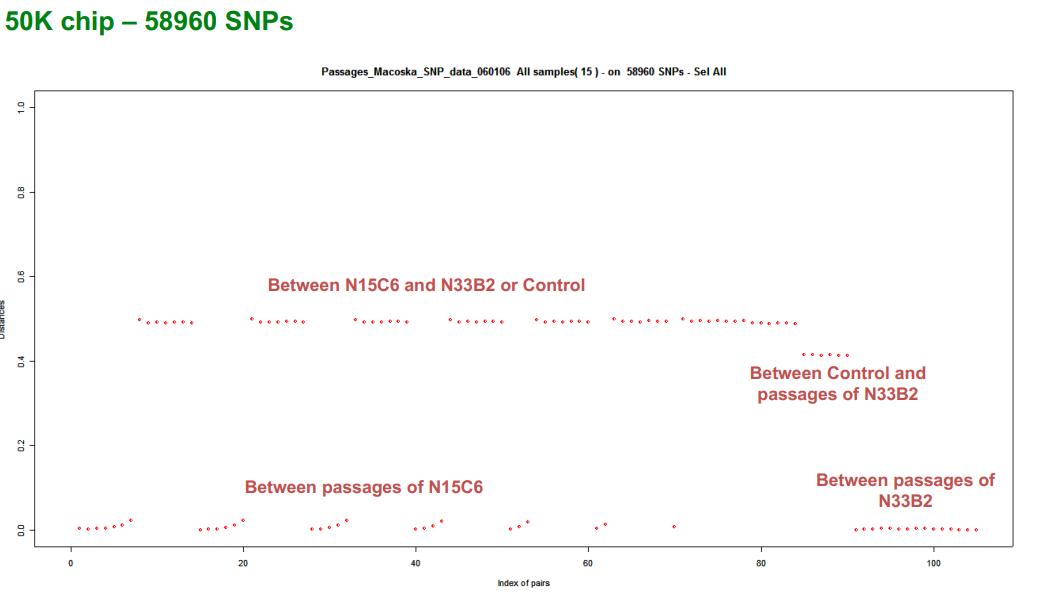
\includegraphics[width=0.6\textwidth]{50k.png}\quad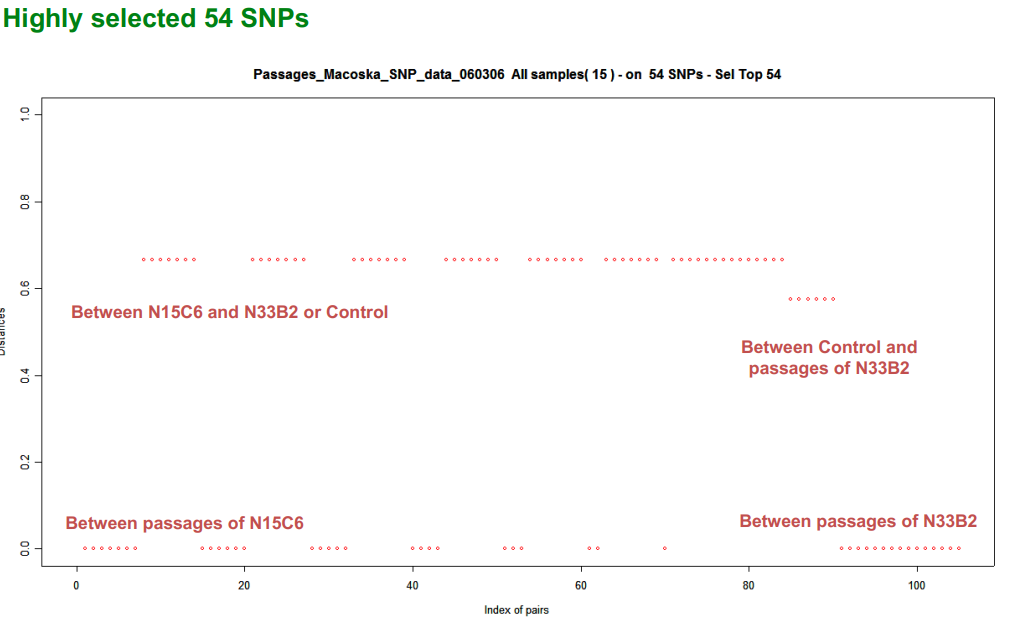
\includegraphics[width=0.6\textwidth]{54_snps.PNG}
	\caption{\label{fig: cell_lines}}
\end{figure}


In the example \ref{fig: cell_lines}, two types of prostate cell lines which underwent multiple passages were used: N15C6 (passages from 48 to 63) and N33B2 (passages from 21 to 39).
The cell lines were profiled with a SNPs array and the assay was run.\\
All passages of each cell lines were compared with all other passages. We expect all passages to have the same genetic fingerprinting in the same cell line.  
\\
However the results obtained using the full array of SNPs (50k), showed that some pairs which should be exactly identical (distance equal to zero) are actually a bit different (points at the bottom-left).
By contrast, by using a set on only 54 SNPs, this diversity is not detectable, indicating  that using the perfect number of SNPs could make us loose some information. 
\\

In order to understand this increase of distance, they looked at each chromosome to see if there were problems that justified increase the increased distance expected to be equal to zero in that cell line. All chromosome were tried. If we focus only on the SNPs spread across Chromosome 11, we observe that there is a major difference for certain passages with respect to the initial ones, only for one cell line (N15C6). This was due to the way the cells were immortalized (insertion in chromosome 11).

\subsection{Individual's Relatedness (genotype-distance)}
The HapMap consortium sequenced hundreds of individuals for different ethnicities and also used trios. Trio sequencing is a technique which involves the sequencing of the genome of mother, father and son/daughter. Trios provide major information for haplotype blocks, for identifying regions related to inheritance, ecc. 

% immagine slide 43
\begin{figure}[H]
	\centering
	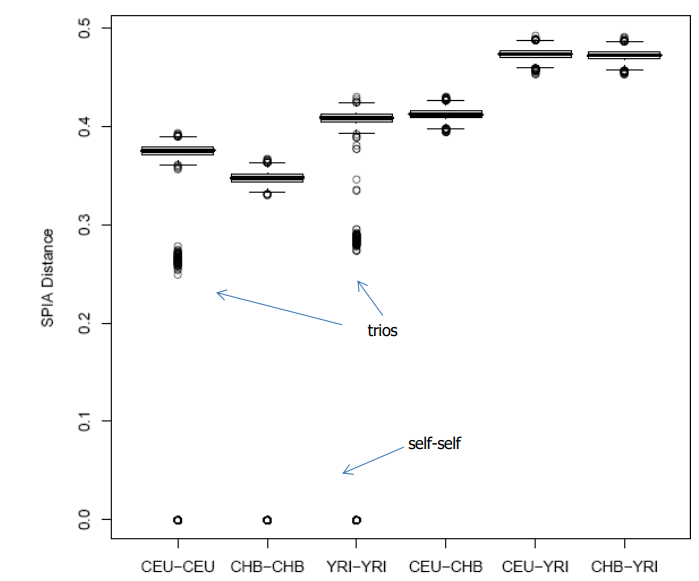
\includegraphics[width = 0.7\textwidth]{relatedness.PNG}
	\caption{\label{fig:trios}}
\end{figure}

By looking at the data based on SPIA Assay (a genotype base assay which measures distance) at figure \ref*{fig:trios} we see that self-self pairs have distance zero, as expected; samples within each ethnicity have a certain average distance, which is lower that the distance observed among different ethnicities. Differences in distance among mixed samples are due to the fact that the SNPs used had on average higher MAF in some populations than in others. We also notice that in trios the distance is not 0 and is not equal to the median distance of unrelated individuals. This can be used for paternity tests or even in forensic science.

\subsection{Example 3: Cancer susceptibility test}
The data showed refers to a study were they were looking for polymorphisms that increase the likelihood of prostate cancer. In these studies, if relatives are present in the cohort, only one of them is taken to avoid skewing the results. \\
When looking for signs of cancer susceptibility by performing genetic fingerprinting, the division based on the degree of relativeness was determined 'for free' and could be used to remove unwanted samples from the cohort.


\subsection{Genetic structure of the human population}
One relevant aspect of the human genome is that it contains everything needed to learn about the genetic structure of the human population. 
\\
Understanding the genetic structure of human populations is of fundamental interest to medial, forensic and anthropological sciences. 
\\
Some of the reasons as to why knowing the genetic substructure of data is important:
\begin{itemize}
	\item The goal of association studies is to identify DNA variants that affect disease risk or other traits of interest. However, association studies can be confounded by differences in ancestry.
	\item Misleading results could arise if individuals selected as disease cases have different ancestry, on average, than healthy controls. If in a study all controls are of the same ethnicity and the test is done on an individual of a different ethnicity than the test is biased.
 	\item If we run a GWAS study using two ethnicities and we want to uset the same markers of susceptibility worldwide, it won't work. 
\end{itemize}

Especially in medicine and in the study of human evolution it is important to track the genetic background of individuals that are involved in studies in order to understand if the individuals are form a homogeneous population or from genetically distant ones. \\
More and more, clinical studies must have declarations of the checks and interpretation of the data of the genetic background of the individuals present in the study. It is very important to come to results for which we know exactly what is the applicability. To avoid spurious results, association studies often restrict their focus to a single continental group. 
\\
Advances in high-throughput genotyping technology have improved the understanding of global patterns of human genetic variation and suggest the potential to use large sample sets to uncover variation among closely spaced populations.
One important piece of information to consider when developing methods to understand the genetic structure of a population, is to think in term of variance, which is also relevant for human diseases.
\\ 
Many SNPs have different MAFs in different populations. If we use those, and are able to have all of them in a simple computational way, we could be able to infer what is one individual's genetic background in terms of origins (e.g. chinese origins). 

The easiest mathematical approach to assess how well SNPs can distinguish ethnicity is by using \textbf{Principal Component Analysis (PCA)}. By running a very simple PCA on a set of SNPs including SNPs with different MAF in different populations we can, in a space, distinguish different ethnical groups. And we could also start thinking at individuals' origins. 

How accurately can one predict an individuals geographic-ethnic background based upon his/her genetic barcode?

% study seen in the slides
\subsubsection{Example paper: 'Genes mirror geography within Europe'}

In the \href{https://www.ncbi.nlm.nih.gov/pmc/articles/PMC2735096/}{study seen during lectures} they used a 500.000 (500k) single nucleotide polymorphism array. Information about the country of origin of grandparents, parents and other relatives was used to determine the geographical location that best represents each individual ancestry. \\
They run a combined study where they used a supervised search to find the best SNPs to make inference and then they tested it on another set of individuals. \\
By using high confidence data (individuals with high confidence origin data) and by using the genotypes of highly informative SNPs for specific region-related inheritance, they were able to rebuild the map of some of the countries in Europe \ref{fig:PCA_countries}. 

% immagine paper 
\begin{figure}[H]
	\centering
	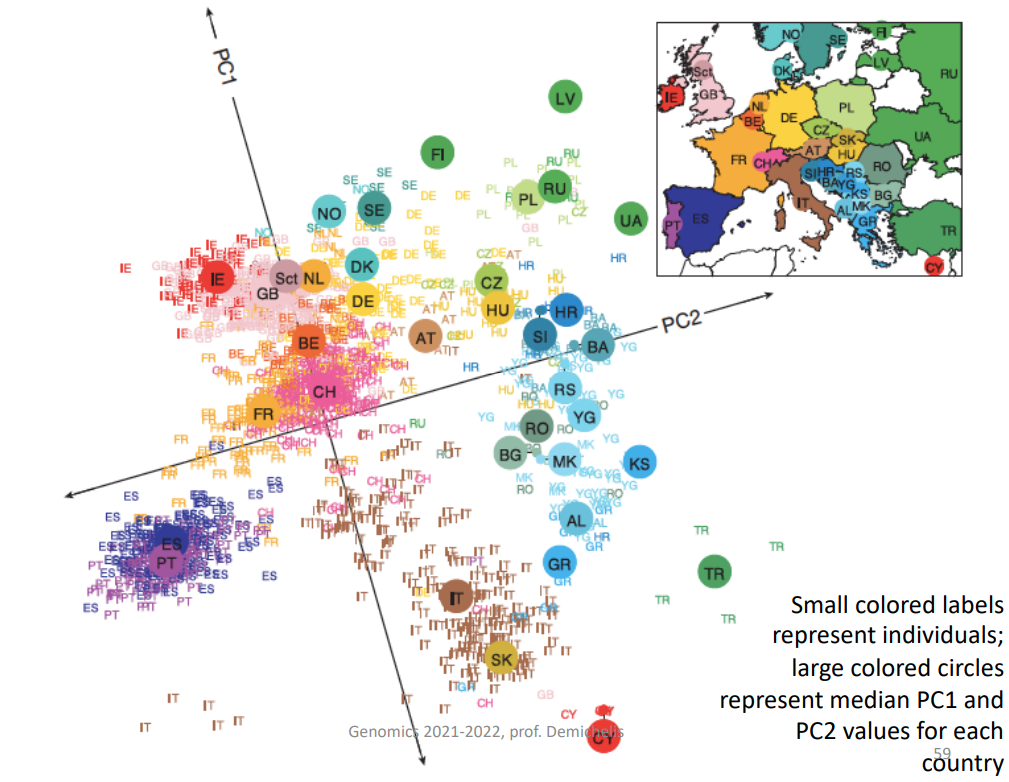
\includegraphics[width=0.7\textwidth]{population.PNG}
	\caption{\label{fig:PCA_countries}}
\end{figure}

This result might be a little bit of a push, but it is true that by using properly selected variants it is possible to distinguish individuals coming from different countries. The way those SNPs are selected is very similar to the process saw for genetic fingerprint, but pushing for the selection of variants that are different in terms of MAF in different populations. 

Clusters that are a bit more dense and distant from the others (like the Spain/Portugal cluster) could be due to the fact that many SNPs selected are typical of that area and are therefore able to maximize the difference with respect to that area (so it is a data-related 'issue').

% immagine 
\begin{figure}[H]
	\centering
	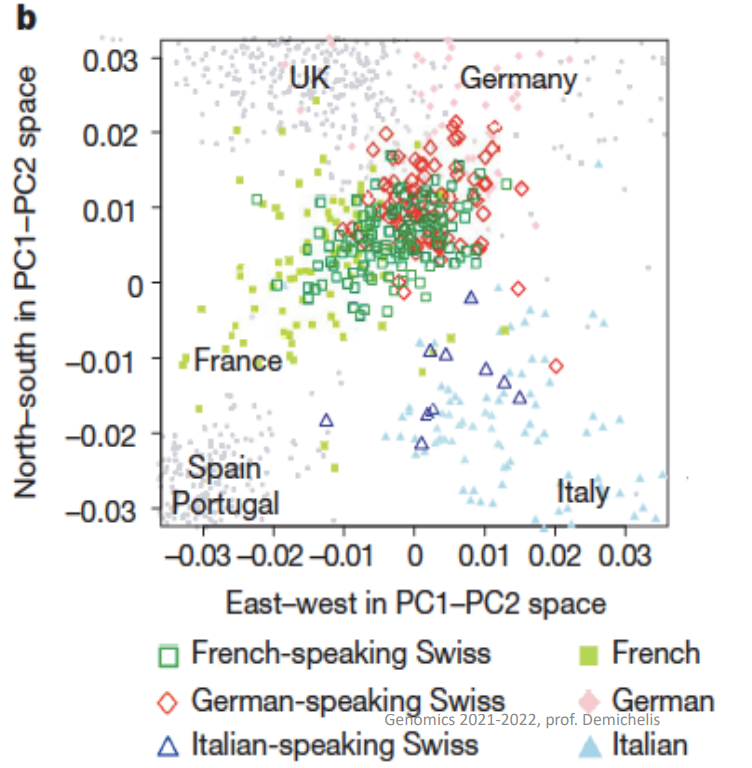
\includegraphics[width=0.5\textwidth]{swiss.PNG}
	\caption{\label{fig: PCA_swiss}}
\end{figure}

Focusing on Switzerland, they could even make inference on the linguistic canton \ref{fig: PCA_swiss}. Again this is a bit of a push, but it is possibly true that in country where some regions have very different habits (e.g. marriage within the same area) might lead to have similar genetic fingerprint. 


\subsubsection{Summary and notes}
Low-frequency alleles tend to be the result of a recent mutation and are expected to geographically cluster around the location at which the mutation first arose. Hence, they can be highly informative about the fine-scale population structure.

Despite low average levels of genetic differentiation among Europeans, close correspondence between genetic and geographic distances was
found. When mapping the genetic basis of a disease phenotype, spurious
associations can arise if genetic structure is not properly accounted for.


    \graphicspath{{chapters/IGVImages/}}

\chapter{IGV (Integrative Genomics Viewer)} \label{chap: IGV}

\textbf{\textit{Written by Maurizio Gilioli}}

\section{Main characteristics}
The human genome nowadays is being explored extensively thanks to exons and
whole-genome sequencing, epigenetic surveys, expression profiling of coding and
noncoding RNAs, single nucleotide polymorphism (SNP) and copy number profiling,
and functional assays. Those findings are essential to pave the way for the
future \textbf{precision medicine}, which is an approach for desease treatment
and prevention that takes into account individual variability in genes, living
environment, and lifestyle for each person. The scope is to administer the right
drug, at the right time and at the right dose for each individual. 

Below, some of the main utilizations of IGV, also represented in figure
\ref*{IGVusages}.
\begin{itemize}
  \item \textbf{NGS alignment}
  \item \textbf{Epigenomics studies}
  \item \textbf{Copy number evaluations}
  \item \textbf{RNA-sequencings}
  \item \textbf{Identification of variants and genotypes}
\end{itemize}

\begin{figure}[H]
    \caption{All the important usages of IGV}
    \centering
    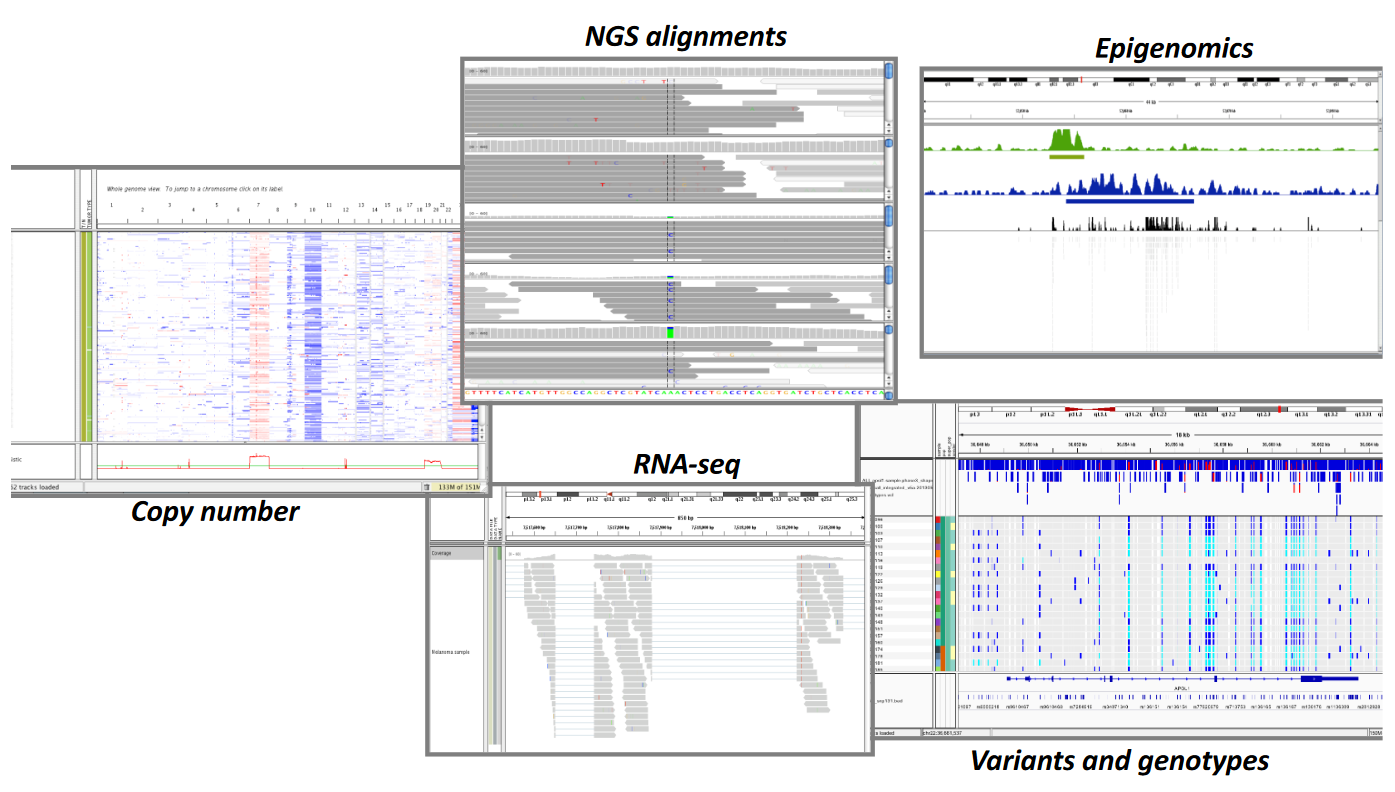
\includegraphics[width=0.8\textwidth]{usagesIGV.PNG}
    \label{IGVusages}
\end{figure}

The IGV software is an \textbf{high-performance lightweight visualization tool}
for interactive exploration of large, integrated genomic datasets. It supports a
\underline{wide variety of data types}, including next-generation sequence data,
and genomic annotations. Data sets can be loaded from local or remote sources,
including cloud-based resources.\\

It allows to move, zoom in and out quickly over different genomic scales
(subfigure \ref*{subfig: IGVnavigation}), and also to jump in precise positions
of the sequence. It is possible to search for genomic coordinates or gene names.
For each resolution scale (“zoom level”), the aggregated data is divided into
tiles (subfigure \ref*{subfig: TileV}) that correspond to a region viewable on a
typical user display. Each tile is subdivided into bins, with the width of a bin
chosen to correspond to the width represented by a pixel at that resolution
scale. The corresponding data tiles for each zoom level are stored in the binary
Tiled Data Format, or TDF, which has been optimized for fast tile retrieval.\\ 
\textit{A tiled data file (\textbf{TDF}) file} (.tdf) is a binary file that
contains data that has been preprocessed for faster display in IGV. TDF files
are generated by using the \textit{igvtools} package (\textit{toTDF} command).\\


\begin{figure}[t]
        \centering
        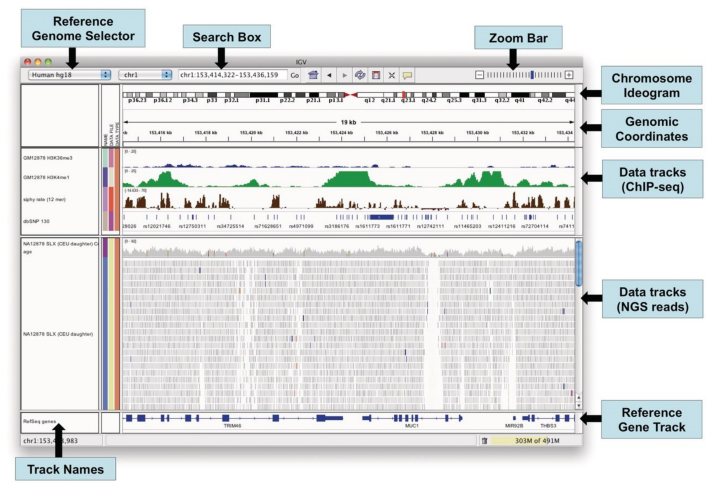
\includegraphics[width=1\textwidth]{IGVview.PNG}
        \caption{IGV interface main features}
        \label{subfig: IGVnavigation}
\end{figure}
\begin{figure}[t]
        \centering
        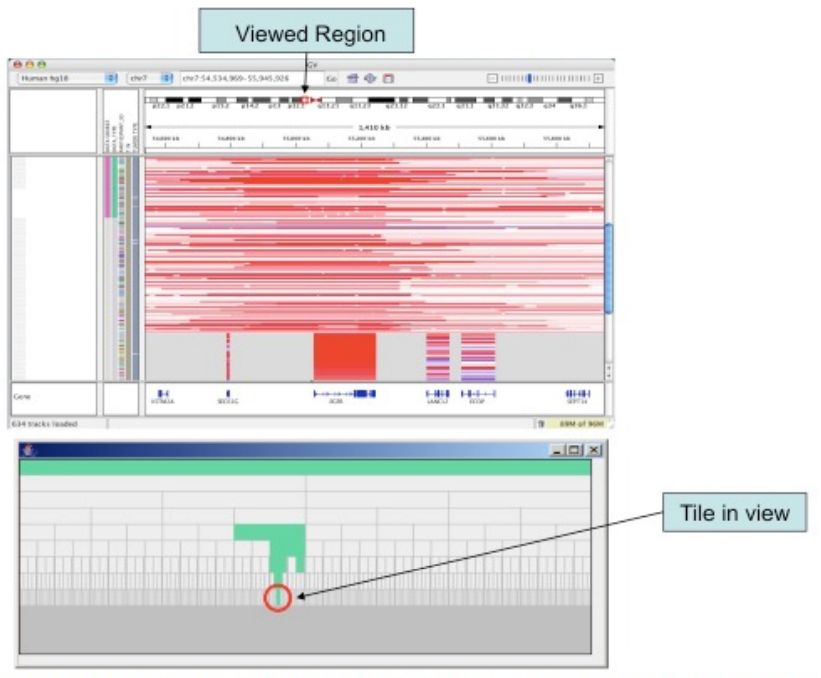
\includegraphics[width=1\textwidth]{TileView.PNG}
        \caption{Tiles view in IGV}
        \label{subfig: TileV}
 
\end{figure}

Importantly, \textbf{tile} sizes for each zoom level are constant and small, and
also, a single tile at the lowest resolution (spanning the entire genome) has
the same memory footprint as a tile at the very high zoom levels (might span
only a few kilobases). \\
Tiles no longer in view are discarded as needed to free memory. Navigation
through a data set is similar to that of \textit{Google Maps}, allowing the user
to zoom and pan seamlessly across the genome at any level of detail from whole
genome to base pair.\\

\textbf{Pixel resolution errors}, occuring when data density exceeds the
constraint given by the number of pixels available for display, could be solved
through data aggregation. As the user zooms below the ~50 kb range, individual
aligned reads become visible. It is possible then to zoom further, and see the
bases at each position.\\
 
Annotations for specific genomes could be found consulting the UCSC Table
Browser \href{http://genome.ucsc.edu/cgi-bin/hgTables}{(UCSC table)}.\\

Other information regarding IGV are present in the
\href{https://authors.library.caltech.edu/72234/2/nbt.1754-S1.pdf}{Supplementaty
information - Integrative Genomics Viewer} pdf file.

\begin{figure}[H]
    \caption{}
    \centering
    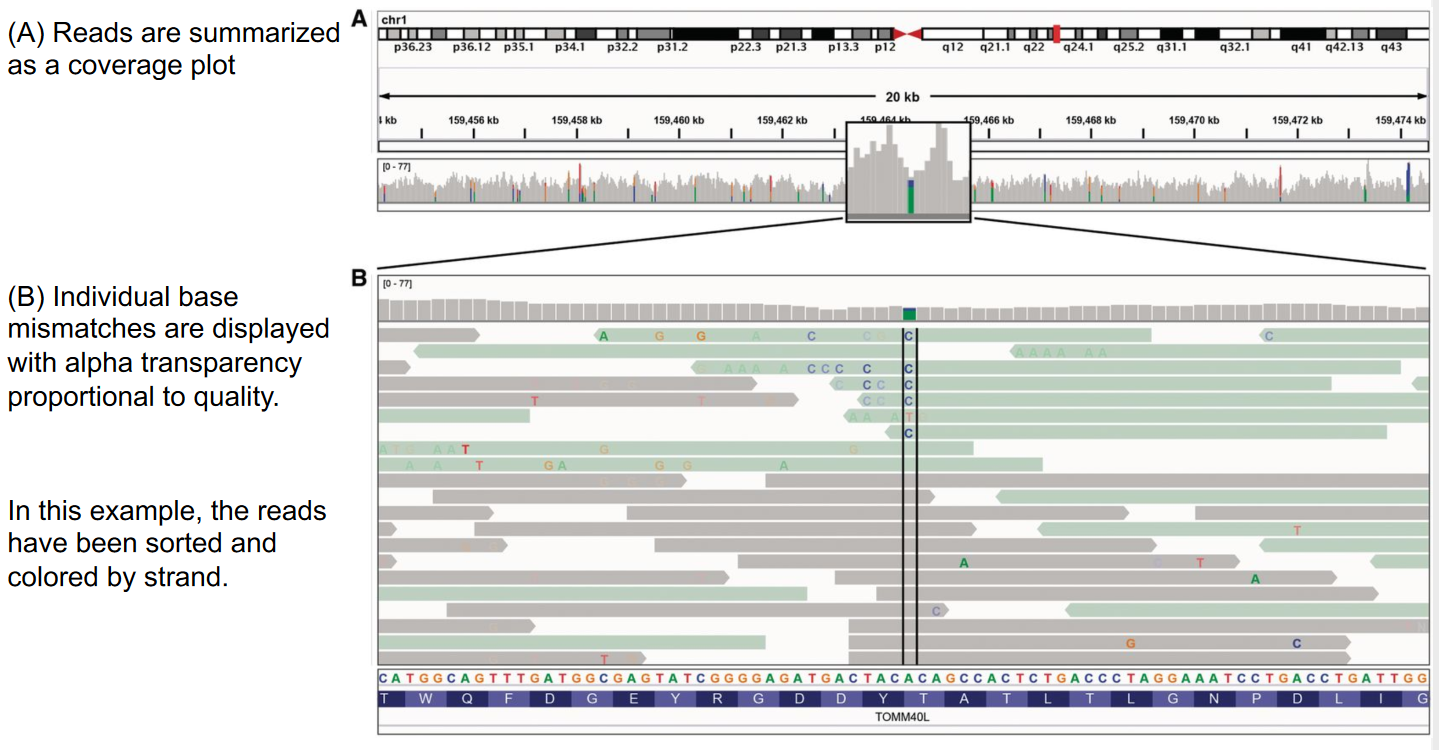
\includegraphics[width=1\textwidth]{IGVReadsView.PNG}
    \label{ViewReads}
\end{figure} 


\subsection{Igvtools}
\textit{Igvtools} comprises a set of utilities to prepeare large files for efficient
display.

\begin{figure}[H]
    \caption{igvtools possible operations, the "count" function allows to generate coverage data, and it takes in input a BAM file. The obtained 
    file could be then loaded with the "Load pre-computed coverage data" commandq}
    \centering
    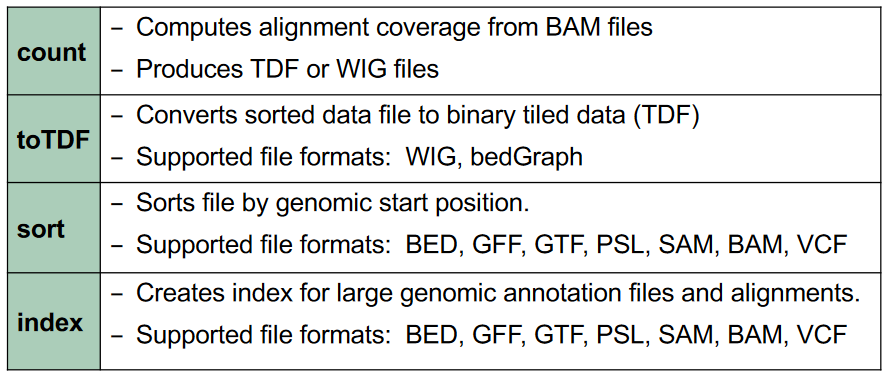
\includegraphics[width=0.7\textwidth]{igvtools.PNG}
\end{figure}

\subsection{Session Files}
Sessions are an integral part of IGV, allowing users to share their data and
views with other users simply and accurately. Session files describe the session
in \textbf{XML}.

\begin{figure}[H]
    \caption{Structure of the XML file}
    \centering
    
\includegraphics[width=0.8\textwidth]{structureXMLfile.PNG}
    \label{XMLfile}
\end{figure} 


\section{Some of the main utilizations}
\textit{(I will not write down all the passages needed to obtain the figures
represented below, as they are included in the exercise file delivered by the
professor)}

\subsection{RNA-seq alignments}

\begin{figure}[H]
    \caption{the height depends on the quantity of reads connecting the different exons.}
    \centering
    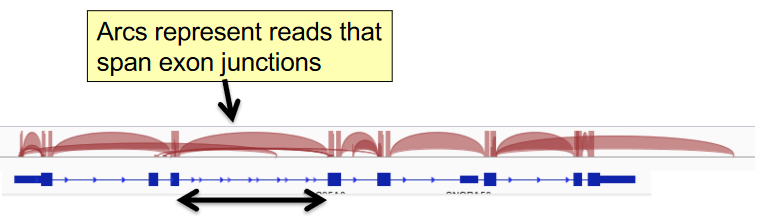
\includegraphics[width=0.8\textwidth]{RNAseqAlign.PNG}
\end{figure}

\begin{figure}[H]
    \caption{\textbf{Sashami plots}: The number of reads connecting exosomes are
    represented here on the curved lines. The peaks represent coverage within
    exons.}
    \centering
    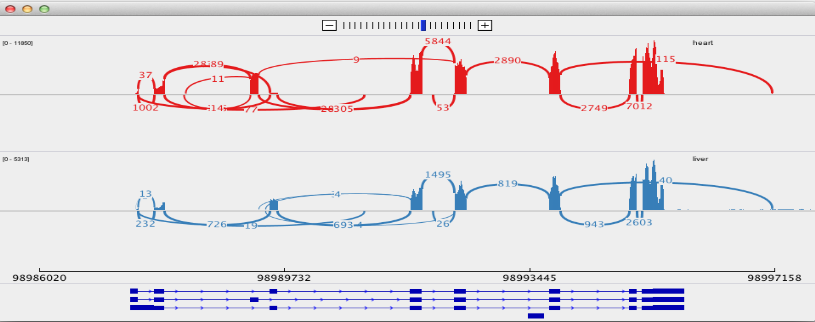
\includegraphics[width=0.8\textwidth]{sashamiplot.PNG}
\end{figure}

\subsection{Study of variants}
It is possible to study variants from different samples.

\begin{figure}[H]
    \centering
    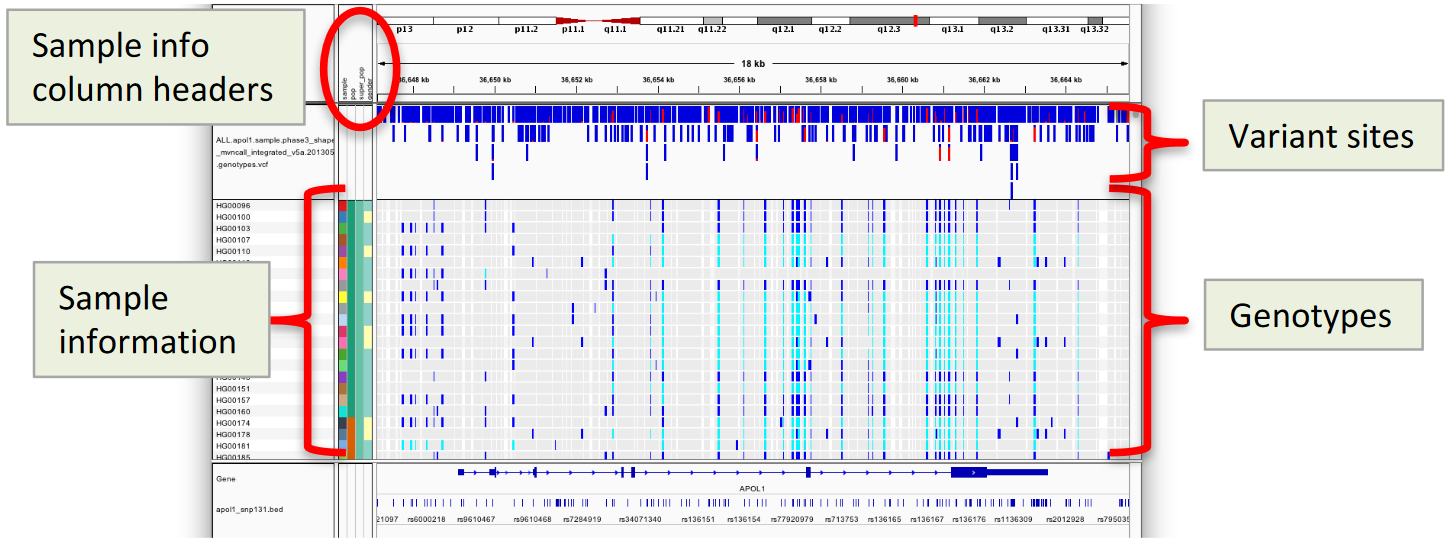
\includegraphics[width=0.9\textwidth]{variantsView.PNG}
\end{figure}

It is also possible to sort the samples in different ways and to group them
considering different characteristics.



\section{Exercise}

The goal was to read pairs/end order/coverage/insert sizes at following
coordinates (hg19). Interpret, if possible, as inversion, inverted duplication,
tandem duplication, or deletion.

\begin{figure}[H]
  \caption{Tasks performed}
  \centering
  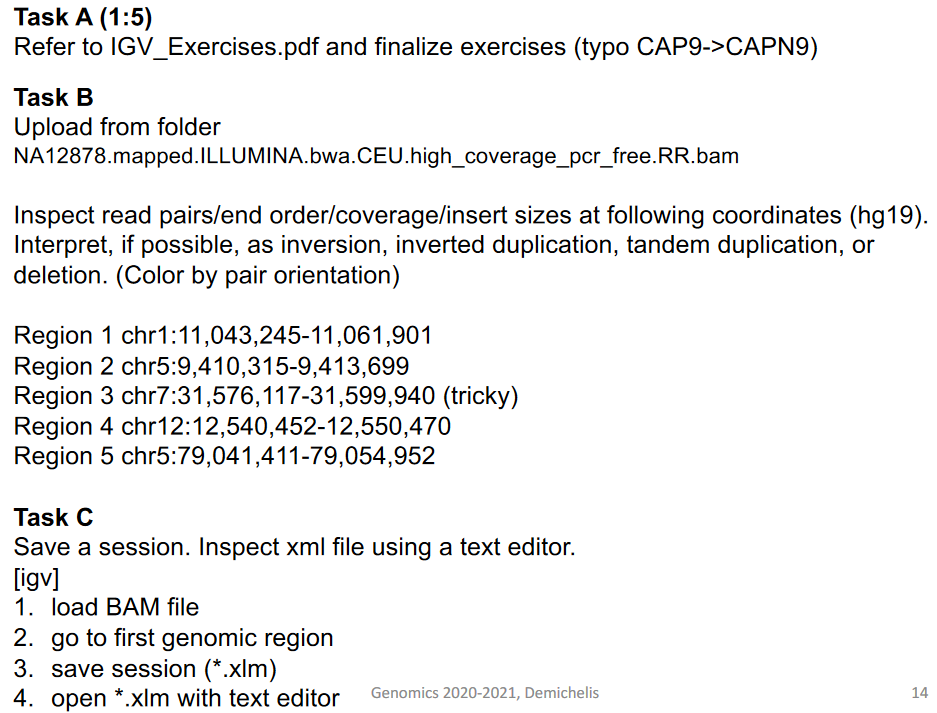
\includegraphics[width=0.8\textwidth]{TasksClass.PNG}
  \label{fig: Tasks performed IGV}
\end{figure}

\subsection{Task B}

\begin{figure}[H]
    \caption{\textit{\textbf{chr1:11,050,009-11,055,137}}: It could be a tandem
    duplication on one of the two alleles and a deletion on the other allele.
    The reason why I would suggest the presence of a deletion is due to the fact
    that the coverage remains quite constant, despite of the duplication.}
    \centering
    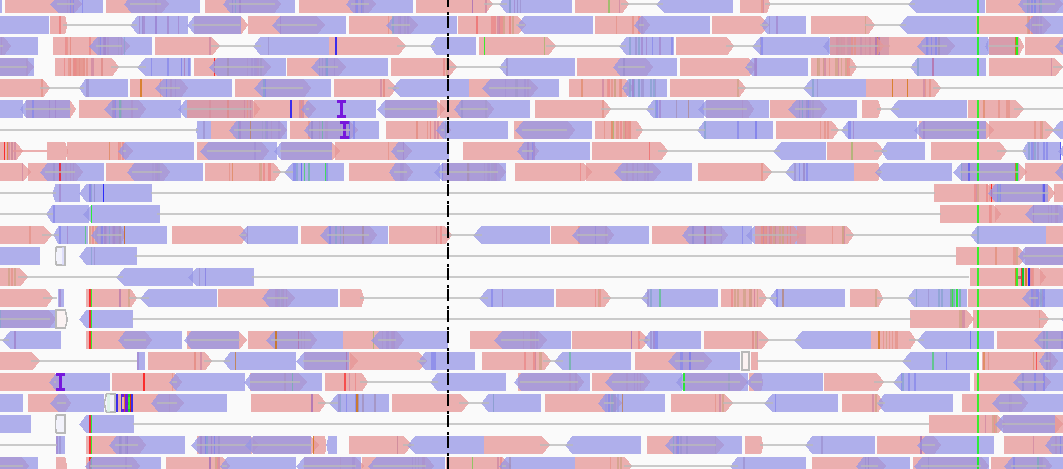
\includegraphics[width=0.8\textwidth]{pos1.PNG}
\end{figure}

\begin{figure}[H]
    \caption{\textbf{\textit{chr5:9,410,315-9,413,699}}: it is quite clear that
    both the alleles were deleted in that region, because of the decrease in
    coverage}
    \centering
    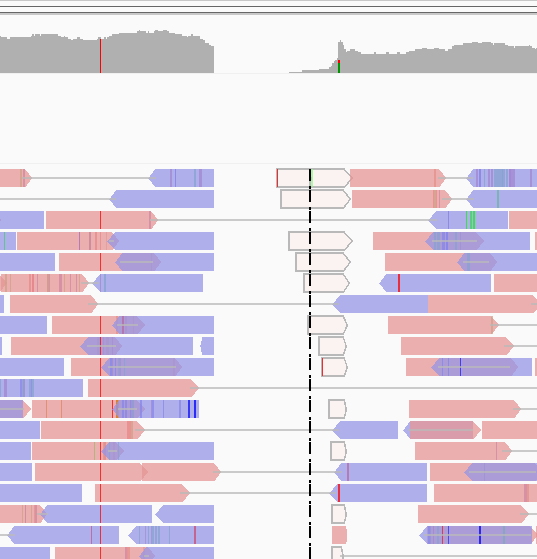
\includegraphics[width=0.8\textwidth]{pos2.PNG}
\end{figure}


\begin{figure}[t]
   \centering
   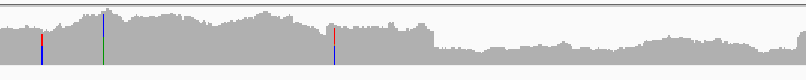
\includegraphics[width=1\textwidth]{cov3.PNG}
\end{figure}

\begin{figure}[t]
  \centering
  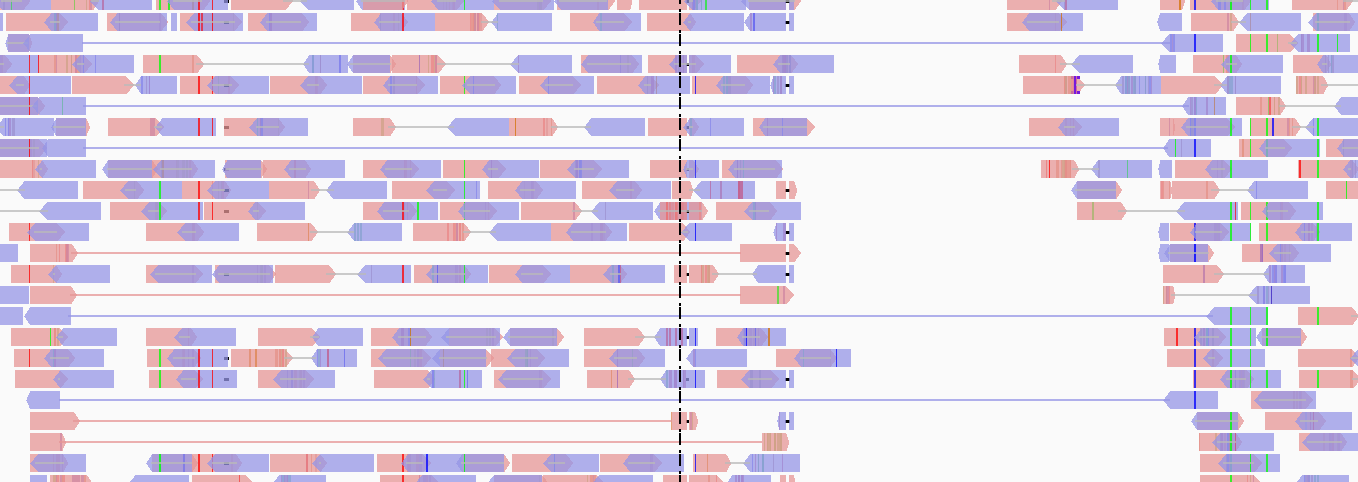
\includegraphics[width=1\textwidth]{pos3.PNG}
\end{figure}

 \begin{figure}[t]
   \centering
   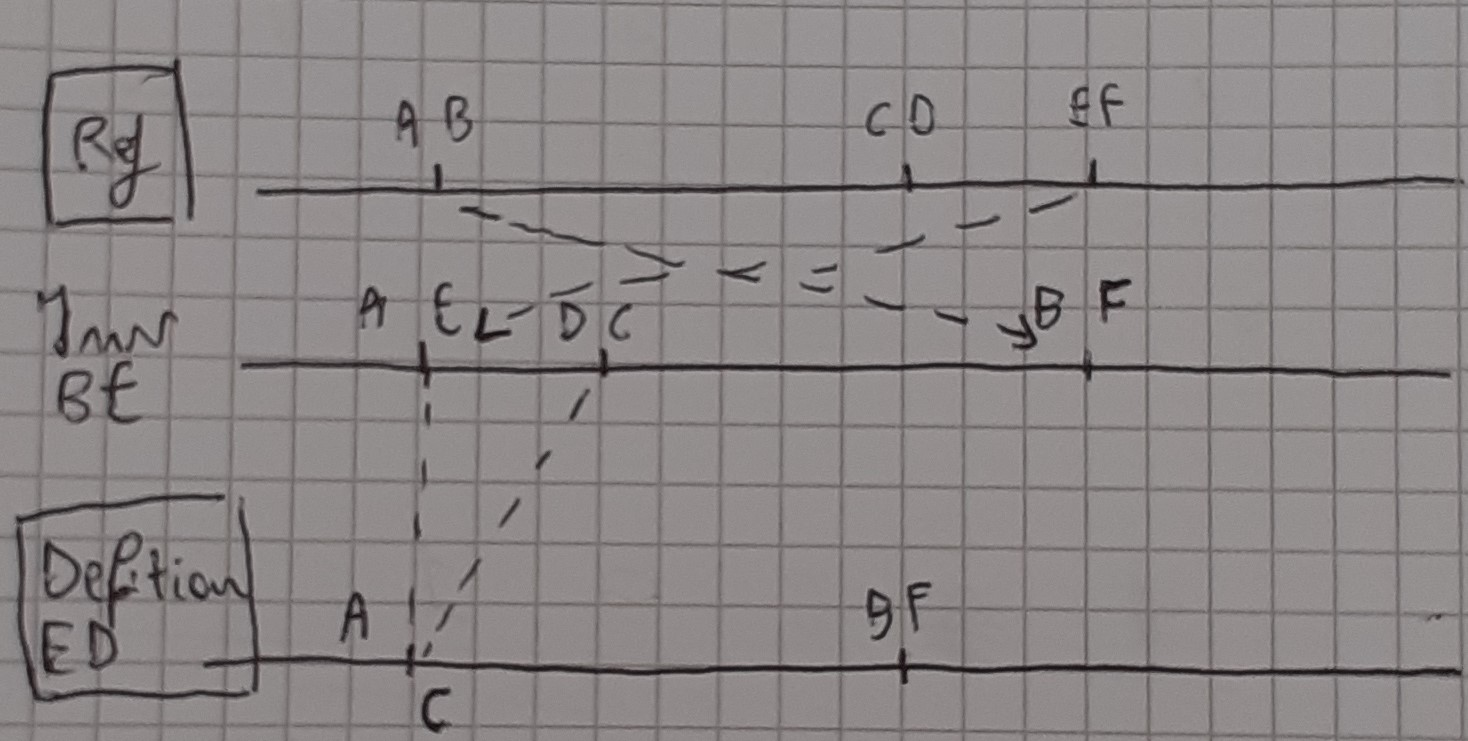
\includegraphics[width=1\textwidth]{pos3passages.jpg}
    \end{figure}


%#TODO complete all the figures of the exercise #TODO it could be a good idea to
%expand this part with some information. Let me know.


    \graphicspath{{chapters/04/}}

\chapter{Tumor Evolution Studies via NGS data}
Tumor board: organism research oriented (and not) hospitals, patient not strictly assigned to one doctor but many specialist. E.g. oncologists, pathologists, geneticists... These boards are also a training asset for complex case studies and teach young doctors how to manege difficult events.
\\
\section{Tumor evolution}
%reference paper Tumour heterogeneity and resistance to cancer therapies
It is important to understand what are the somatic events that occur during tumor genesis/evolution and when they arise.\\
Cancer cells accumulate mutations due to both cell division and toxic agents (radiations, UV light,…); these mutations are maintained by the cell and lead to clonal expansion.  We can have a driver mutation kicking an oncogene or multiple mutations. 
Typical traits of cancer are:
\begin{itemize}
\item Cancer is a dynamic disease, that's why evolution of the disease is so important to track.
\item During the course of disease, cancers generally become more heterogeneous, which is often related to treatment resistance.
\item The bulk tumor includes a diverse collection of cells harboring distinct molecular signatures with differential levels of sensitivity to treatment.
\item This heterogeneity might result in a non-uniform distribution of genetically
\item distinct tumour-cell sub-populations across and within disease sites (spatial heterogeneity) or temporal variations in the molecular makeup of cancer cells (temporal heterogeneity)
\end{itemize}

\subsection{Tumor heterogeneity}
Every site of the genome with somatic mutations (point, inversion, …) is going to be differentially represented in tumor samples. Heterogeneity provides the fuel for resistance and is an obstacle to cancer treatment.
\\
Therefore, an accurate assessment of tumor heterogeneity is essential for the development of effective therapies. Emerging techniques to study with considerable potential to dissect the complex clonal architecture of cancers heterogeneity are: multi-region sequencing, single cell sequencing, analysis of autopsy samples, and longitudinal analysis of liquid biopsy samples.
\\
\\

However, techniques to study tumor heterogeneity are hindered by intra-patient heterogeneity, which divide into \textbf{spatial} and \textbf{temporal} heterogeneity. 

\paragraph*{Spatial heterogeneity}
	The patient has several independent tumor masses, which share certain cells, but have a unique genetic makeup;

\paragraph*{Temporal heterogeneity}
	One mass changes content over time, naturally or under particular pressures.


\begin{figure}[H]
	\centering
	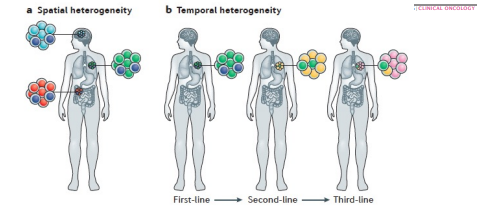
\includegraphics[width=0.7\textwidth]{heterogeneity.png}
	\caption{a) Spatial heterogeneity denotes an uneven distribution of cancer subclones across different regions of the primary tumor and/or metastatic sites. b) Temporal heterogeneity refers to variations in the molecular makeup of a single lesion over time, either as a result of natural progression of the tumor or as a result of exposure to selective pressures created by clinical interventions. Colors denote the presence of subclones with different genetic features.}
	\label{fig:hetero}
\end{figure}

\begin{figure}[H]
	\centering
	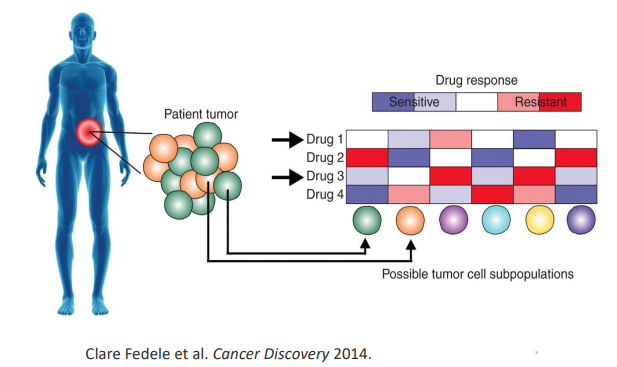
\includegraphics[width=0.6\textwidth]{treatment.png}
	\caption{x Certain cells of the tumor mass respond to treatment and some don't. Red = cell resistant to drug, blue = cell sensitive to drug. }
	\label{fig:hetero}
\end{figure}

\subsubsection{Linear an branching evolution}
It could be possible that some cells positively respond to treatment and others not, creating a heterogeneous population in the mass.
\\
The features of this set of cells changes over time. This evolution happens either because the new population \textbf{replaces} the older, or there's a \textbf{branching} and the tumor mass becomes heterogeneous.\\

\paragraph*{Linear evolution}
Sequential genetic alterations confer a fitness advantage such that successive generations are able to outcompete the preceding clones, which lack this fitness advantage. Surviving dominant clones harbor the ancestral mutation.

\paragraph*{Branch evolution}
Multiple genetically distinct populations can emerge from a common ancestral clone, with certain subclonal populations diverging from the common ancestor before others. The branching evolution is depicted in figure \ref{fig:branching}.

\begin{figure}[H]
	\centering
	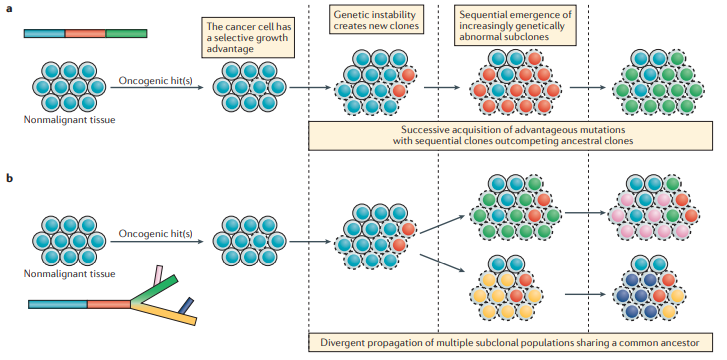
\includegraphics[width=0.7\textwidth]{branching.png}
	\caption{ a) everything branches out from the monoclonal origin, but b) polyclonal origin, independent metastatic processes. Cells from independent lesions meet and form a highly diverse metastatic tumor.}
	\label{fig:branching}
\end{figure}

How can we study tumor evolution? Example seen in class: prostate sample, multiple independent lesions. By browsing through the morphologies, we can find similarities for the expression of the same gene. Sanger sequencing can be used for very specific mutations. Through bulk DNA sequencing from each position, a representation of the tumor burden and features of all the different areas can be obtained.

\subsection{Treatment resistance}
How does resistance to treatment arise in cancer cells? Is treatment resistance encoded in the original cells or is it driven by the treatment itself?
\\
The two possibilities (also reported in figure \ref{fig:response}) are selection of clones tat provide resistance, or transformation of clones under treatment pressure. \\

\paragraph*{Primary resistance}
Pre-existing heterogeneity fosters resistance. Only susceptible cells die and resistance cells continue dividing, allowing the tumor to regrow (high mass tumor).

\paragraph*{Acquired resistance}
Drug-tolerant, “persister” cells generate resistant clones. At the time of diagnosis there are no markers, the de novo resistance alteration is developed afterward. Eventually, the resistant cells can from new tumors not responding to the drug.


\begin{figure}[H]
	\centering
	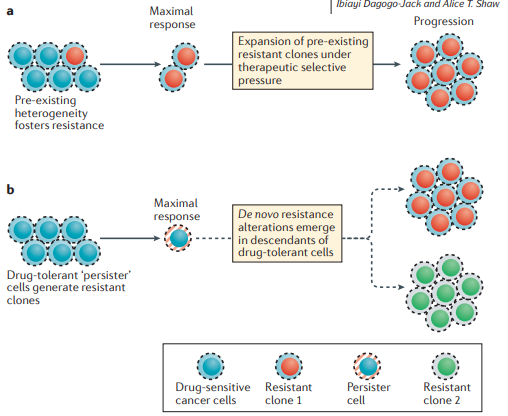
\includegraphics[width=0.7\textwidth]{response.png}
	\caption{ Tumor cells evolution driven by treatment.}
	\label{fig:response}
\end{figure}

\section{From sketches to sequencing data evolution information}
In order to study tumor evolution, we can use common and private lesions across multiple samples from the same individual to reconstruct the path. 
Conversely, we can learn from multiple individuals at the same time points (select the most clonal lesion), with the goal of building a common clonal evolution map.
E.g. tumor suppressor gene NKX3-1 and PTEN lesions are shared between many individuals. Overall, in prostate cancer it is likely to have a subsequent PTEN mutation if CHD1 mutation is present.
\\
In general, we are interested into finding out which lesions occurred first and which is the model that fits better the data.

\subsection{Tumor evolution and heterogeneity}
To summarize, there are the difficult tasks one has to deal with when studying tumor data, and always need to study and take into account:
\begin{itemize}
\item intra tumor heterogeneity;
\item inter tumor/intra patient heterogeneity;
\item Inter-patient heterogeneity;
\item clinical/treatment relevance;
\item time dependency;
\item admixture DNA (tumor purity);
\end{itemize}

If properly investigated, they provide for insightful hints int he analysis.

\subsubsection{Admixture}
Whenever we take a piece of tissue from a patient, we have multiple cell types. The same happens with a biopsy, which will never be composed 100\% by cancer cells. This concept is referred to as \textbf{DNA admixture}.
\\
\textbf{Tumor purity} is computed as 1-DNA admixture. Purity is related to lesion aggressiveness (low purity is linked to less severity) and lesion classification (clonal or subclonal). In fact, every interpretation of somatic data needs to be interpreted in the context of tumor purity. Lesion is clonal if all tumor cells have it, a less present lesion instead might be subclonal.

%Deconvultion looking at NGS data. Lesion 100\% pure if the contamination of the adm of tumor cells is very low. \\

\section{Useful measures from NGS pipeline}
Also in this case we will be exploiting the polymorphic information that is present in the genetics of every individual. SNPs are very helpful in all somatic analysis.
\begin{itemize}
\item \textbf{Minor allele frequency, (MAF)}, frequency at which the alternative allele at a polymorphic site is represented in the population.
\item \textbf{Allelic fraction, (AF)}, how many times at a specific locus in a single individual we see the alternative base being represented. How many reads represent the alternative allele, how much support. 
\end{itemize}

\subsection{Informative SNPs in cancer studies}
Informative SNPs are SNPs at which one individual has a heterozygous genotype; we can count allelic fraction and assess the proportion of reads supporting the alternative base. 
If we have a deletion spanning a genomic area, at every informative SNP we will see that the allelic fraction, instead of being 50, will be either 0 or 100. Therefore, a diseased tissue will have an allelic distribution peaking at 0 or 1.
\\
\textit{Nref} is the percentage of reference base in the non-deleted allele.
\\
We can also track \textbf{beta ($\beta$)}, the percentage of neutral reads. If both alleles are equally represented, beta will be equal to 1. 
Conversely, when only one allele is represented, beta is equal to 0. 
How much beta is different from 1 is an indication of either admixture or subclonality of the lesion.
When only some cells in the sample are tumor cells, the distribution of AF will have two peaks. 
\\
In each genomic segments that we are studying we many informative SNPs, at least two, to drive some conclusions. For example, figure \ref{fig:af_properties}.\\
How do we select informative SNPs? Use dbSNP database and select all heterozygous genotype sites, patient-centric analysis regardless of MAF. Obviously in the case of a target assay, it is possible to enrich for SNPs for high MAF, maximizing likelihood of finding informative SNPs (should be carefully designed).

\begin{figure}[H]
	\centering
	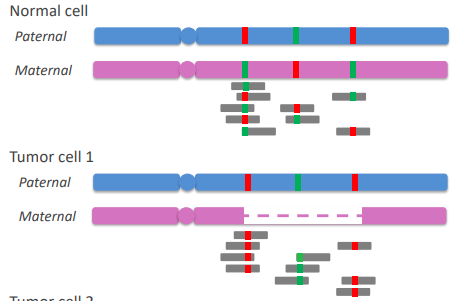
\includegraphics[width=0.5\textwidth]{af_properties.png}
	\caption{ Thanks to the presence of informative SNPs is very easy to detected the loss of an allele in the tumor cell.}
	\label{fig:af_properties}
\end{figure}

An example of the use of AF and beta measures for tumor data analysis in depicted in figure \ref{fig:a_b}.

\begin{figure}[htbp!]
	\centering
	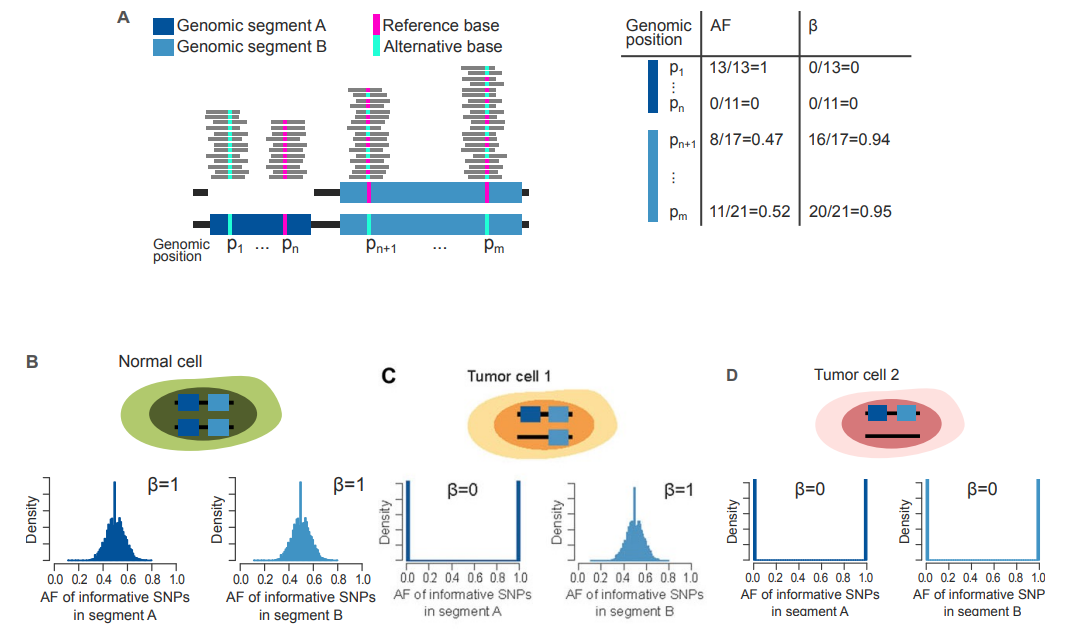
\includegraphics[width=0.8\textwidth]{a.png}
	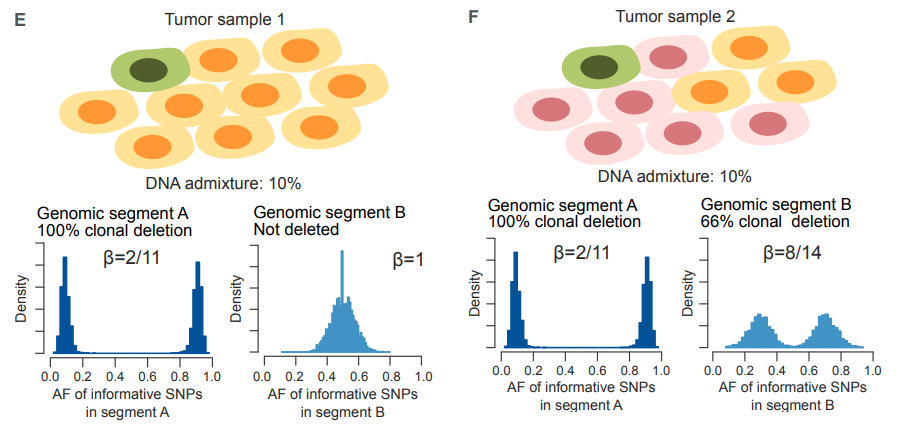
\includegraphics[width=0.8\textwidth]{b.png}
	\caption{ 
	\textbf{A)}Example of the allelic fraction (AF) and beta ($\beta$) in computed in five genomic positions ($p_1$ to $p_m$). Positions $p_1$ to $p_n$ are within a hemizygous deleted genomic segment A, while genomic positions $p_{n+1}$ to pm lie within a wild type genomic segment B.\\
\textbf{(B-D)} Examples of a normal cell and two different tumor cells. Tumor cells 1 and 2 differ for the status of genomic segment B. Histograms below cell cartoons report the expected distribution of the allelic fraction of SNPs in genomic segments A and B together with the associated beta values.\\
\textbf{(E-F)} Examples of two different tumor samples. Tumor sample 1 includes one normal cell and nine tumor cells with deleted genomic segment A and wild type genomic segment B. Tumor sample 2 differs from tumor sample 1 in the presence of six tumor cells with a hemizygous deletion of genomic segment B.
Expected distribution of the AF of informative SNPs together with estimated beta are depicted below each tumor sample cartoon.}
\label{fig:a_b}
\end{figure}

\subsection{Coverage and AF properties}
Does the mean coverage of the experiment impact on the ability to use the AF properties?\\
Intuitively, the deeper the sequencing the more likely it is to distinguish distribution that are not so close to each other. It is especially important when $\beta$ is close to zero. An example is shown in figure \ref{fig:beta}.


\begin{figure}[H]
	\centering
	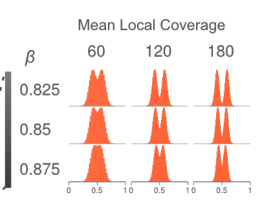
\includegraphics[width=0.4\textwidth]{beta.png}
	\caption{2X experiment: on average we have 2 reads per gene, very easy to miscall.\\
10X experiment: easy to do call, but in the case of tumor cells it becomes difficult. The higher the sequencing depth, the more accurate the calls will be (as it becomes easier to tell when a distribution has two peaks).
}
\label{fig:beta}
\end{figure}

\subsection{Computing Beta}
We can compute beta for each genomic segment S:
\begin{enumerate}
\item compute the observed distribution of the AF of informative SNPs in the genomic segment S;
\item find the values of Beta and Nref such that the expected distribution of the AF matches the observed AF;
\item compute uncertainty around Beta as a function of:
	\begin{enumerate}
	\item the mean coverage of S;
	\item the number of informative SNPs in S;
	\end{enumerate}
\end{enumerate}


\section{Global vs Local Estimates of admixture}\label{sec:admixture}
We'll discuss two types of sample and how to determine the differences in cell population (admixture).
\\
In sample one depicted in figure \ref{fig:sample1} there's a clonal cell population, meaning no heterogeneity. On the X axis we have genomic coordinates indexed by informative SNPs for that individual, on the Y axis the half AF.
\\
For all the informative SNPs present in this chunk of DNA, we see drops in AF that are smaller or wider, but more or less similar for each one of those lesions (drops). Meaning a drop or a gain in the amount of DNA that is almost identical in all of these chunks. \\
The representation of the lesions is supported by the same data along the stretch of DNA.
Thinking in terms of how much the AF distribution from 0 and 1 and the center is basically the same across all of them. Meaning, the level of admixture, both globally and locally, is the same. \\
Or, again, the amount of cells that have the first, second, third lesion etc. is the same.

\begin{figure}[H]
	\centering
	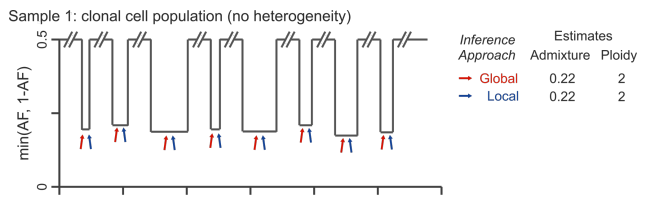
\includegraphics[width=0.7\textwidth]{sample1.png}
	\caption{In the clonal cell population how much the distribution deviates from AF is the same globally and locally.}
	\label{fig:sample1}
\end{figure}

In picture \ref{fig:sample2} below we can see another sample.
We can clearly discover multiclonal cell population. The depth of the lesion is proportional to the number of cells that carry the lesion.
In this case the definitions of local and global admixture change: a \textbf{global} value is a global value of tumor purity, a local value is a value of the clonality of the lesion in the diseased cell population.

\begin{figure}[H]
	\centering
	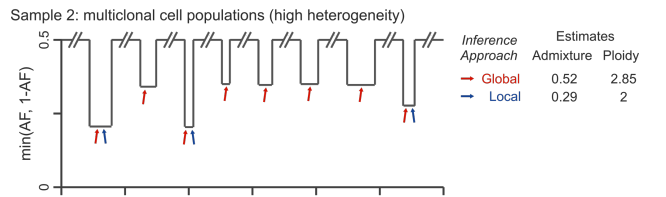
\includegraphics[width=0.7\textwidth]{sample2.png}
	\caption{We observe heterogeneity, the global and local values are different. A global value is relative to tumor purity, local to clonality. Admixture = 1-tumor purity}
	\label{fig:sample2}
\end{figure}

\subsubsection{Estimate of DNA admixture (1-Purity)}
We will now translate the concepts expressed in the previous sub-sections \ref{sec:admixture} in a 2-dimensional space, as shown in figure \ref{fig:2d}.

\begin{wrapfigure}{l}{0.5\textwidth}
	%\centering
	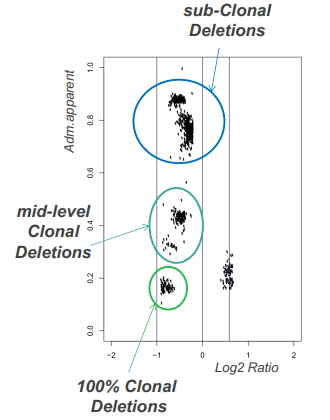
\includegraphics[width=0.7\linewidth]{adm.png}
	\caption{Multiple clusters, where each dot is a genomic segment. Lower clusters are used for the admixture, the others are subclonal.}
 \label{fig:2d}
\end{wrapfigure}

On the X axis we have the Log2 ratio measure and on the Y axis the admixture apparent, which is proportional to the beta  value.\\
The Log2 Ratio is basically tumor over normal in the log2 space. It allows to interpret info about every segment int he genome when coupled with the beta measure.
\\
The admixture apparent is calculated as 

\begin{equation} \label{eq:adm}
\textit{Adm. apparent} = \frac{\beta}{2-\beta}
\end{equation}

This measure associates an apparent DNA admxiture to each monoallelic deletion. It is useful to calculate the clonality values, for which the formula is: 

\begin{equation}
\textit{Clonality:} \frac{1 - \textit{Adm. apparent}}{1 - \textit{Adm. global}}
\end{equation}

The lowest cluster is the one used to assess admixture and the other ones are subclonal lesions.\\
Moreover, the closest the points are, the most probable it is that the lesions happened close in time, and viceversa.

\section{A challenging case (PR-2741*)}
Data of a real case of prostate cancer in which we can see a clear drop in coverage in region 2 of the 5th chromosome, while region 1 and 3 have equal coverage. The DNA present in region 2 could come either from admixing cells or from cells that do not have the deletion. \\
Looking at the AF of region 1, 2, 3, both from the tumor and the match normal normal sample we observe more or less the same two modes of distribution.\\
In the tumor sample in fact we do not see two peaks in 0 and 1 as expected. It could be signal of intervening normal cells, that bring the modes to the center, or subclonality event. \\


\begin{figure}
	\centering
	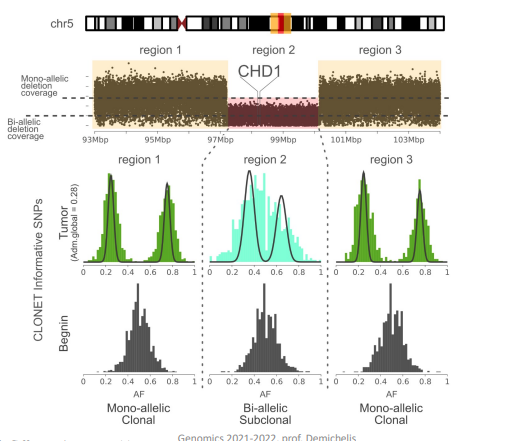
\includegraphics[width=0.7\linewidth]{PR_2741.png}
	\caption{ The distribution of heterozygous SNPs in benign cells is peaked in 0.5, while we observe two modes in tumor cells. The distance between the two modes is equal in 1 and 3, it’s proportional. In the middle we see that the two modes are moving towards the center, suggesting that the deletion is not likely 100\% clonal or it is clonal and shift is due to lack of deletion in 1 and 3. Subclonality: lesion with admixture}
	\label{fig:adm}
	\end{figure}


























    \graphicspath{{chapters/TumorEvStudiesIIImages/}}
\chapter{Tumor evolution studies (continued)}

\textbf{\textit{Written by Giorgia Bucciarelli}}


\section{Recalls from the previous lecture}

At the basis of tumor evolution is the concept of how to use {informative SNPs}:
SNPs for which a specific individual has heterozygous calls so that set of SNPs
is unique for every individual.

This property is connected to the fact that when we have the loss of an allele,
the allelic fraction of the informative SNPs within that lesion will be
informative of the lesion and its depth (clonality = what's the fraction of
tumor cells that very likely harbor that lesion).

We can also have different population of cells, when a set of lesions is present
in every population it is said to be clonal whereas when a specific set of
lesion is harbored only by a subpopulation it is defined as subclonal.

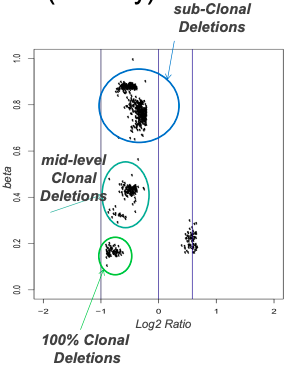
\includegraphics[width=2.37708in,height=2.94375in]{image1.png}\emph{Estimate of
DNA Admixture}\\

\emph{{Log2 Ratio}} is the log2 of the ratio of the tumor over the normal that
applies to array data signals (intensity of the signals) but also to the local
coverage of a tumor BAM file over a normal BAM file.

In the figure each dot is a genomic segment or a gene that clusterize in the
space and when dots are in a same cluster it means that they very likely share
the same copy number status and also the same level of clonality.

\emph{{Beta}} is a variable that goes from 0 to 1 and provides information of
the number of reads that equally represent the two alleles; when beta is equal
to 1 the concept of admixture (1-purity) is equal to 1 meaning that purity is
equal to 0 if we are at the top of the y scale it means that there's no signal
related to tumor content, while the lower we go, so the closer we get to 0, the
higher the tumor content and the level of clonality is.

If we use this equation we can assess the level of clonality of a cluster.

So the graph in the figure puts in relation the copy number status (log2 ratio)
and the purity/clonality of the sample (Beta); the more we go towards the left
the fewer number of copies, the lower on the y axis the higher the clonality.

The best proxy of the quantity of tumor content present in a sample is done
using the lowest cluster.

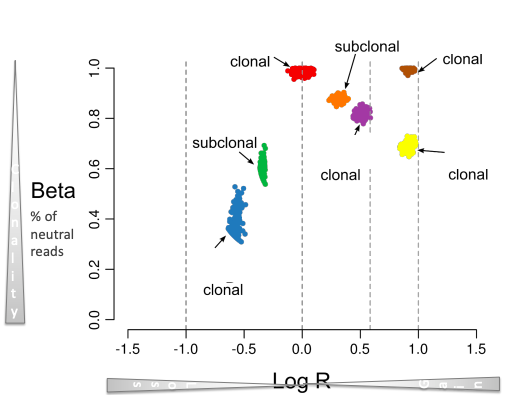
\includegraphics[width=3.46875in,height=2.65139in]{image2.png}\\

We have losses and
gain of DNA copies, moving on the x axis.

The beta is related to the clonality so the lower we go the more clonal the
signal is.

The only difference from the previous figure is the presence of extra clusters:

\begin{itemize}
\item
  The blue cluster with deletions is the most clonal one
\item
  Both blue and green clusters had deletions, since they have a negative log2
  ratio, but the green ones are less clonal than the blue ones
\item
  In log2 R = 0 and ß = 1, where there's the red cluster, we have a status of no
  copy number changes (wild-type status in terms of copy numbers). This
  basically represents a total number of alleles which is the same in both the
  tumor and normal sample.
\item
  All the other clusters with a positive log2 ratio had a gain of DNA
\end{itemize}

\includegraphics[width=2.72153in,height=2.08958in]{image3.png}\\

In this figure the number of copies that correspond to all the clusters in the
space is also reported.

\begin{itemize}
\item
  Blue one: one copy of DNA, so we have a deletion
\item
  Green one: also one copy of DNA but with subclonality
\end{itemize}

This is how we can map in the space the status of clonality and the number of
copies for a specific segment in the genome.

So again, the lower we go the more clonal the clusters are, the more left the
deeper they are in terms of loss of DNA.

We can use these information to build \emph{{evolution maps}}.

The first thing to do is to look, within each individual, at concomitant
deletion where one is subclonal to the other one.

\includegraphics[width=3.18859in,height=2.21348in]{image4.png}\\

In the figure:

\begin{itemize}
\item
  In sample 1 the brown lesion is subclonal to the orange one, and that same
  lesion is also subclonal to the green one.
\item
  In sample 2 we have again the support of the relation between the brown and
  orange lesion with the same level of subclonality (brown subclonal to orange).
\item
  In sample 3 is the same as in sample 1 and 2.
\item
  Samples 4 and 5 have the same concomitant green and brown lesions again with
  the same level of subclonality.
\item
  In sample 5 only we also have another concomitant lesion (blue subclonal to
  brown).
\end{itemize}

So we perform this analysis for all the concomitant lesions in our sample and we
start drawing the arrows to keep track of what is subclonal to what. We compile
this list across all individuals and look for how many times we see support for
the same relationship in the same direction.

In our case we can say that the relationship going from orange to brown is
supported by 3 out of 5 individuals; the same can be said for the green going to
brown. The blue one is instead not significant since it's supported by only one
individual.

So having multiple observation supporting that aberration x precedes aberration
y (i.e. aberration y is subclonal to aberration x) we can build an evolution
chart.

\includegraphics[width=2.38194in,height=2.40417in]{image5.png}\\

The orange and the green which have no relationship between them, are at the
same level on the x axis in the path and they both go into brown.

So one can assume that the more clonal a lesion is the more likely it is that it
occurred earlier during the evolution (time is on the x axis of the path), and
we can look for recurrent relationships among lesions.

In principle we can say that the grey ones at the beginning happened at the same
time point and then at a second time point, the tumors in our set of samples,
underwent loss of orange and green genes and then later they both underwent loss
of the brown gene.

\includegraphics[width=2.63403in,height=1.74097in]{image6.png}\\

If we do that in
large datasets (lung cancer melanoma, prostate cancer \ldots) we can come up
with all the dependencies that were observed and that were supported by more
than one individual (e.g. in prostate cancer we can say that a loss in NKX3-1
precedes the deletion of PTEN).

Even if we have hundreds of BAM files on whole exon sequencing data from large
collections all that we can build are evolution maps with at most three layers
(pretty disappointing).

This has multiple reasons, one of them is that:

\begin{itemize}
\item
  To build a relationship which is statistically significant between two genes
  we need to have multiple instances of that relationship (in many samples)
  which means that we need to have co-occurrence of the two lesions and
  subclonality of the second lesion with respect to the first in a significant
  number of individuals compared to the total number of individuals that have
  co-occurrence. So if co-occurrence occurs in N individuals and subclonality of
  the second lesion to the first one occurs in a fraction of those, only if this
  fraction is significant with a proportion test out of the total number, then
  we can build the path.
\end{itemize}

Therefore we are tremendously limited by co-occurrence of lesions.

To boost the reconstruction of these paths gene families or pathways have been
exploited.

E.g. if we are dealing with PTEN which is a tumor-suppressive gene relevant in a
specific pathway (PF3K), then it doesn't matter if we have deletion or
inactivation of the same genes in the same pathway, what matters for the tumor
evolution is that that specific pathway is altered and so what we can do is
start aggregating signals from genes that belong to the same pathway.

So if individual 1 has a relationship between gene A and some gene in a specific
pathway (PF3K) and individual 2 has a relationship between gene A and a second
gene in that same pathway, then we can assume that maybe they have the same
effect and so we can aggregate the information on the landing gene.

So instead of going from gene 1 to gene 2 we go from pathway 1 to pathway 2, and
in terms of numbers what we gain is that the co-occurrences are counted
including all the gene lesions with the same function in pathway 1 and all the
gene lesions with the same function in pathway 2 (if we consider the
inactivation of the gene then we have to consider all the lesions that
inactivate the gene and not others).

We can then run a simple test to build our path.

With this method we start having some more data to look for major changes during
the evolution of the tumor pathway.

E.g. in prostate cancer we'd identify a set of pathways that are more or less at
some level altered in earlier staged disease and that then trigger or are
precedent to our pathways. Doing so we can learn more in terms of the biology of
the disease evolution.

We can also decide to go for a mix model or a mix approach, where for certain
genes we go at the pathway level while for other we treat them separately.

There are also more complicated ways to make inference of tumor evolution. Some
try to avoid the hypothesis that the more clonal a lesion is the more likely it
is to happen early, because we know it's not always the case; it might be in
untreated samples but not in treated samples. In a treatment regiment, because
of drug pressure selection, specific resistant clones harboring a specific
lesion can take over due to their higher rate of proliferation, so in this case
if we see a lesion that appears to be more clonal it doesn't really mean that it
happened earlier, it may be that it had a higher proliferation and so it's
taking over (and we see it as apparently clonal but it's in fact a late event)
-\textgreater{} important concept in precision medicine.

So simplicistic approaches like the one discussed are proper for untreated (in
terms of drugs) primary diseases.

Evolution charts can also be boosted via the combination of multiple molecular
layers.

\section{Ploidy and purity correction on $\log_2(\frac{T}{N})$ data}

\emph{How can we use measure of the tumor purity and the effect of the tumor
ploidy?}

\emph{How can we compare two different samples for which we quantify completely
different levels of tumor content?}

E.g.: we have a sample a 100\% pure and with 50\% of clonality (a lesion present
in 50\% of the cells) and a second sample with a tumor purity of 10\% and a
clonality of 100\% (a lesion present in 100\% of the cells), we need a way that
allows us to compare numbers without having to convert everytime for every
lesion the depth of the lesion based on the tumor content, so we need an
equation that we can apply to every individual data that puts everything on the
same level

(same concept as gene expression normalization).

The coverage makes data coming from different samples comparable because we
normalize everything to the total coverage, but when we deal with diseased cells
we can have contamination from the admixture, so we need an extra step.

The step, once we know how to assess the tumor purity and ploidy, is quite
simple: we need to adjust the data for tumor purity and ploidy.

\emph{Schematically}

\includegraphics[width=3.79931in,height=5.42569in]{image7.png}\\

In the figure we are looking at one tumor sample: a whole genome sequencing of
one melanoma sample.

We see multiple peaks which correspond to different copy number states.

Let's suppose we have a genome with a backbone of three copies but we sequence a
bulk and we don't have 100\% purity but 80\% (so 20\% is contamination).

\emph{\textbf{Ploidy correction}}

Computationally we assess the ploidy through the copy number space and then
correct the data.

From the tumor and the normal we obtain something like the first graph, and we
could wrongly assume that the main peak is always in 0 (wild-type state of the
genome), but it shouldn't.

In fact, if we assess the ploidy and overall we see a backbone state of three
copies for our genome, then the main peak should be shifted toward three.

So, the \emph{ploidy correction shifts the distribution} towards the right
(second graph).

\emph{\textbf{Purity correction}}

We correct our data and the \emph{{purity correction causes a stretch between
the peaks}}, since tumor admixture dilutes the signal. So, the effect of purity
correction is a wider spread between the peaks (third graph).

+ add the example graph

\begin{itemize}
\item
  If we have one extra copy in our tumor, the log2 ratio will be around 0.58 and
  so we would expect that the signal will peak around that value; for two extra
  copies we'd expect a peak around 1 and so on.
\item
  We'll have the peak of the normal state around 0 and then if we have an
  underrepresented allele in our tumor we'd get another peak around -1 for the
  hemizygous deletion and then the homozygous deletion.
\item
  If our signal is not 100\% pure tumor (so diluted by normal cells), the peak
  at -1 and 0.5 would be closer to the 0 peak for uncorrected data.
\end{itemize}

\emph{{When we correct for tumor purity we stretch the distribution to go to the
correct positions.}}

E.g.: 25 whole genome sequencing of melanoma samples

\includegraphics[width=3.42917in,height=4.56111in]{image8.png}\\

\begin{itemize}
\item
  1\textsuperscript{st} graph: The distribution of the log2 data of uncorrected
  signal, every melanoma sample is highly aberrant with a ploidy that is
  different between different individuals and a purity that is also different
  between different individuals. But we do have the tumor ploidy and purity so
  we can correct the data.
\item
  2\textsuperscript{nd} graph: we correct for ploidy
\item
  3\textsuperscript{rd} graph: we correct for purity too
\end{itemize}

If we don't correct our data we'll see much noise (as in the first graph).

From the corrected data we learn that:

\begin{itemize}
\item
  A lot of tumors have a backbone ploidy of two
\item
  There are some hemyzigous deletion not perfectly centered in one but closer to
  one in the 3\textsuperscript{rd} graph if compared to the
  1\textsuperscript{st}
\item
  Some signal is compatible with homozygous deletion
\item
  Whave a reasonable amount of signal for three copies which could come from a
  threeploid status of some tumors.
\end{itemize}

These corrections are part of standard preprocessing.

\emph{\textbf{Tumor Ploidy and Purity adjustment, corrected TCGA data}}

\emph{How commonly does suboptimal tumor purity affect proper copy number data
analysis?}

\emph{How common it is that purity is not equal to 100\% and ploidy is not equal
to 2 in any primary disease}

\includegraphics[width=3.24375in,height=3.97569in]{image9.png}\\

In the figure we can see a list of tumor types, where every draw is a tumor type
(lung carcinoma, bladder cancer, colon cancer, ovarian ecc.). On the x axis we
have tumor purity (1-admixture) going from 0 to 100\% and for each type we can
see the distribution of the tumor purity analysis of all the samples from the
TCGA dataset.

Every tumor type has a different number of sample profile

Looking at the GBM (glioblastoma multiforme), the middle vertical line is the
median signal of the distribution, there are outliers shown and the black
horizontal line represents the interquartile range.

Altogether across 27 tumor types they were able to assess the tumor cellularity,
clonality and all in about five thousand of those, meaning that a great fraction
of those had some optimal data (very strict criteria)

\begin{itemize}
\item
  The majority of the median distributions are above 50 \%.
\item
  The overall tumor cellularity was almost 70\%.
\end{itemize}

\emph{If we look at ploidy: what is the fraction within each tumor type with a
ploidy significantly above two}?

In the graph they are sorted by decreasing percentage of tumors with a ploidy
higher than two; for example, for the first and second tumor type, more than 50
\% of the primary tumors have a ploidy status above two so either they underwent
whole genome duplication (4 or more copies) or at least we have three.

Then we have some tumors with very low ploidy (blue dots) where at least one
copy of the entire genome is completely lost -\textgreater{} low allele specific
ploidy assessment.

The figure shows what happens to data when we correct for ploidy and purity

\begin{itemize}
\item
  \includegraphics[width=3.65972in,height=3.76389in]{image10.png}\\
  On the y axis
  we have the log2 ratio
\item
  On the left side we have the raw data
\item
  On the right side the adjusted data
\end{itemize}

We can see where correction for ploidy and purity takes the signal.

Focusing just on the first half we can see that

we have the same noise we've seen for the melanoma uncorrected data.

\emph{The correction of the data results in the reclassification of 30\% of the
totality of the segments} (if we don't correct we have a wrong copy number
classification in 30\% of the cases)

Then there are certain copy numbers which are more or less affected by these
corrections.

What's interesting is that the correction led to the doubling of the homozygous
deletions that we were able to observe (these are very important because it
means that the proteic product won't be there at all).

\textbf{ALLELE SPECIFIC ANALYSIS (CNA, CNB SPACE)}

\includegraphics[width=3.12639in,height=4.35903in]{image11.png}\\

Thinking in terms of allele specific data:

\begin{enumerate}
\def\labelenumi{\arabic{enumi}.}
\item
  We have unadjusted signal
\item
  We adjust
\item
  Then we can go to the beta-log2 ratio space where we can see that the data
  underneath the peaks are belonging to specific clusters
\end{enumerate}

This suggests that by only looking at the log2 ratio we are unable to
distinguish the presence of clusters with different clonalities.

The most interesting information is the lower cluster (on the x=0 axis):

\begin{itemize}
\item
  Even when the T/N = 1 (tumor/normal ratio) what we can have is a status of one
  copy and one copy or something that equally gives a log2 ratio equal to 0 but
  which still represents copy neutral loss of heterozygosity (CN-LOH), so two
  copies on one allele and zero copies on the other.
\end{itemize}

+ example figures (will be added soon, I have to draw them)

1\textsuperscript{st} figure:

We have the loss of an allele on A so we'll have 2-1-2 copies

2\textsuperscript{nd} figure:

We have the same situation on allele A but allele B is doubled so we'll have
3-2-3 copies

So, in this situation, the gene x will have two copies but both of them coming
from the same allele (B).

Computing the log2 ratio in this situation we'll have the log2(2/2) which will
lead to the collocation on the 0 axis but on the lower part (due to the
clonality).

The log2-beta statuses allows us to distinguish the copy-neutral LOH.

Also for the gain is the same (three copies from the same allele and zero from
the other)

There are equations that allows us to go from here to a space where our
coordinates are the number of copies of allele A and number of copies of allele
B.\\
\includegraphics[width=6.68889in,height=2.97633in]{image12.png}\\
For four copies
we can have different combinations:

\begin{itemize}
\item
  2 copies of A + 2 copies of B,
\item
  3 copies of A + 1 copy of B
\item
  4 copies of A + 0 copies of B
\end{itemize}

The equations are not important, what's important is that once we have corrected
the data then we can shift our analysis up to the level of number of copies of
each allele for each gene.

\emph{Why is this important?}

E.g.: Let's imagine that for gene X we have one copy lost on allele A and a
point mutation on the allele B which leads to unfunctional product so full loss
of the protein.

If we instead are in the second case and the point mutation happened after the
duplication then we'll still have an allele functioning, whereas if it happened
before the duplication, we'd have again full loss of functional protein.

If we are able to distinguish the alleles we are able to also distinguish in
which situation we are (which means we can distinguish between what's functional
and what's not).

\begin{itemize}
\item
  \includegraphics[width=3.00903in,height=2.89861in]{image13.png}\\
  Extra graph
  with the same space allele a/ allele B where we can divide the space in terms
  of total number of copies and also what happens on both.
\end{itemize}

So, this whole computation allows us:

\begin{itemize}
\item
  To reclassificate copy number status in the space by shifting and stretching
\item
  To also assign a copy number A and B to every segment of the genome, which
  means to every gene
\end{itemize}

If we do that we can see that many of the segments that have a total number of
copies equal to two are in fact 2+0 and not 1+1. This means that there is a
significant fraction of the genome which is apparently wild-type but which
actually underwent loss from one an allele and a gain on the other. This event
is called copy-neutral loss of heterozygosity (CN-LOH).

Copy-neutral because the number of copies doesn't change but there's been loss
of heterozygosity.

From the TCGA data, they observed a relevant fraction of high copy number levels
(4-5 copies) which all came from the same allele (one allele was lost and the
other underwent multiple cycles of duplication).

\includegraphics[width=2.29167in,height=2.00347in]{image14.png}\\

So, looking at
the copy number only we'd say there's a gain (which is true) but we wouldn't
have all the complete information (we also have to perform the allele analysis).

These information are relevant in precision medicine because there are ways to
target genes exploiting loss of heterozygosity and up until now it was only used
for deletions but now that's known, even if we have an apparent CN-LOH or we
have a copy number gain LOH we can still consider to use the same approach.

\includegraphics[width=6.58333in,height=5.0625in]{image15.png}\textbf{Case study
-- CNA, CNB real data example with multi-sample data from the same patient}\\

We have one patient and we're looking at a primary sample, for which we plot the
whole sequencing data in the copy number allele space and what we see (from the
first plot) is that:

\begin{itemize}
\item
  There's a cloud of dots (every dot is a gene) which has a total number of
  copies around two
\item
  There's a cluster that underwent hemyzygous deletion so we only have one copy
  of all the genes in there
\item
  There's one gene with a homozygous deletion (0,0).
\end{itemize}

Then we have three other metastatic sites for which they had biopsies so that
they could run whole genome sequencing and perform the analysis of the data in
the same space.

We have a local metastasis and two distant mets.

What we see:

\begin{itemize}
\item
  In distant met 1 there's no homozygous deletion*
\item
  In both the distant mets the gene RB1 gained an extra copy on allele A
\item
  In all the mets there are extra gains of copies of all the genes (maybe
  there's been a whole genome duplication of some sort)
\item
  In distant met 1 the data are as clean as to allow us to state that the data
  point in yellow/grey over the 1 is subclonal (if we have genes with 1+1 copy
  is equivalent to say it's a subclonal hemizygous loss, it means that all the
  cells have at least one copy and then some cells also have a second copy)
\item
  In terms of evolution, very likely extra copies of the whole genome also in
  the local met after the loss of the second copy of the gene
\item
  CN-LOH of many genes, including RB1
\item
  Level of subclonality overall not high
\end{itemize}

*\emph{How's possible that there's a homozygous deletion in the primary tumor
which is then absent in the distant mets?} No DNA can be regained, it's
impossible that the gene is reacquired, so probably the seeding of the distant
mets happened before the loss of the gene.

Another way to track evolution is to have \emph{serial time points.}

\includegraphics[width=6.68889in,height=5.05486in]{image16.png}\\

If we deal with biopsies over time we can track the evolution using the allelic
fraction of a lesion.

E.g.: reasoning in terms of point mutations, let's say we have a point mutation
at time point 0 in certain allelic fractions, which correspond to different
subsets, we track the fractions over time.

Doing this we can make inference of which subsets appear during the treatment
and are taking over (red one in the example figure).

Allelic fraction at any time point needs to be corrected for tumor content,
otherwise we would not be able to compare multiple time points from the same
patient.

    \graphicspath{{chapters/TumorEvolution3Images/}}

\chapter{Tumor evolution studies via NGS data: SNVs-based methods}

\textbf{\textit{Written by Linda Cova}}

There is a large number of tumors where copy-number aberrations are minimal.
Consequently, it is difficult to use copy number based approaches for these
kinds of tumors. It is estimated that about 3\% of primary tumors present flat
genomes, meaning that they display very few copy number changes. These types of
tumors are correlated to a better prognosis both in overall survival and
progression-free interval, but relapses are still present so the assessment of
these tumors is important.

In order to address this issue, some tools were developed to detect tumor purity
via SNVs.

\section{Rationale of somatic point mutation based assays}

\begin{figure}[!ht]
\centering
    \includegraphics[width=0.5\linewidth]{peaks.png}
    \caption{\label{fig:peaks}Peaks shift for a clonal tumor cell population and
    some mixed populations. Considering two genomic locations, healthy cells
    have genotype AA-AA, clonal tumor cells AB-AA and subclonal tumor cells
    AB-AB, where B is the alternative allele associated with a somatic point
    mutation}
\end{figure}

The distribution of allelic fractions of the clonal population only is
symmetric, with the main peak around 0.5. A mixed population of clonal tumor and
normal healthy cells shows a shifted peak. The distance from 0.5 to the peak is
proportional to the fraction of normal cells, because normal cells contribution
moves the peak towards the side from the center (purity shift displayed in
\ref{fig:peaks}. A subclonal point mutation is identified with a second peak
towards 0, because its allelic fraction is probably far distant from 0.5.

\section{TPES (Tumor Purity Estimation)}
\textit{Alessio Locallo (Demichelis' student, 2019)}\\

\begin{figure}[!ht]
\centering
    \includegraphics[width=0.7\linewidth]{tpes.png}
    \caption{\label{fig:tpes}Workflow of the TPES algorithm}
\end{figure}

It is important to consider the \textbf{Reference Mapping Bias}: a polymorphic
locus carrying a non-reference base is less likely to be mapped during the
alignment process. With a perfect SNV (clonal, monoallelic, in highly pure
tumor), allelic fraction will not be 0.5 because the aligner considers the
variation as an error and sometimes discards the read containing it: some signal
is lost.\\

TPES steps:
\begin{itemize}
    \item \textbf{Selection of CN-neutral segments}: point mutations that are
    flat in terms of copy-number are perfect for flat genomes and easier to deal
    with. This is the first filter implemented by this tool: a threshold is set
    on the log2 of the tumor over the normal.
    \item When considering the \textbf{allelic fractions} of all the somatic
    mutations of whole genome, a major peak is expected around 0.5 (expected
    VAF). Other peaks can be originated from things that escaped the previous
    filter or from monoallelic mutations with copy-neutral LOH (loss of
    heterozygosity): in this case the allelic fraction results doubled. So
    another threshold on allelic fraction is needed (maxAF=0.55)
    \item Identification of \textbf{putative clonal SNVs}: the peak closer to
    0.5 is the most useful to determine tumor purity. The others are related to
    subclonal events.
\end{itemize}

With enough point mutations and after peaks identification, purity is assessed
with the following equation:
\[ 1-purity = admixture = 1-\frac{observedVAF}{expectedVAF} \]

\section{How many SNVs are needed to assess tumor purity?}

The number of SNVs changes for each tumor type, so not all tumor types guarantee
enough SNVs. The minimum number of SNVs needed to obtain reliable results can be
assessed with a \textbf{comparative analysis}. The Spearman's correlations
between the results of two different purity calling algorithms uding decreasing
number of SNVs are computed. The subsampling approach (which SNVs to consider?)
is to subsample the SNVs as many time as possible to have higher confidence on
the results. At each iteration, as many samples as possible are used, but the
number decreases when the number of SNVs increases.

The computations determined 10 as the minimum number of SNVs needed to infer
tumor purity. With this number, tumor was detected in 80\% of samples by
combining TPES and CLONET (CN-based). The 20\% could be tumor-free or not
detected samples. Since both SNVs and CN based methods failed, this 20\% could
be possibly detected with methylation.

\begin{figure}[!ht]
\centering
    \includegraphics[width=0.7\linewidth]{comparative.png}
    \caption{\label{fig:comp}\textbf{A}) Correlation between two purity
    estimating algorithms (TPES and CLONET) with decreasing number of SNVs
    considered. \textbf{B}) Percentages of samples where tumor purity was
    assessed by the two tools (TPES considering with 10 SNVs)}
\end{figure}


\section{Comparison between purity callers}

TPES was compared to other tools that do the same thing but with a range of
different methodologies: good correlation between the results was found, in
particular with the CN-based algorithms. This shows that genomics is more
reproducible in general to assess purity, while methods relying for example on
image analysis give different results.

The best solution to assess tumor purity is to couple and CN-based and a
SNV-based approach: some samples are only detected by one of the two so a
combination gives the best results globally.

\section{Pros and Cons of SNVs-based tumor purity assessment}
Pros:
\begin{itemize}
    \item Best-suited for CN neutral tumor genomes
    \item Applicable to a range of NGS techniques
    \item Fast and low demanding in terms of computational resources
    \item TPES is available as R package on CRAN
\end{itemize}
Limitations:
\begin{itemize}
    \item Needs a reasonable number of putative clonal somatic heterozygous SNVs
    per sample
    \item  Sensible to subclonal cell populations which could influence clonal
    peak detection
\end{itemize}

    \graphicspath{{chapters/LiquidBiopsiesImages/}}

\chapter{Liquid biopsies in oncology}
It is more feasible to track the tumor progression stage for a patient from liquid biopsies (panoramic overview at a time point), rather than from tissue biopsy (highly accurate snapshot in a specific site at a timepoint). How accurate can a liquid biopsy is depends on many factors: if there is homogeneity the quality is really similar to tissue biopsy. We might have different representations according to sites. The major advantage of liquid biopsy is being minimally invasive. Furthermore, it is easier for early diagnostics (screening), quantify the presence of minimal residual of disease.

\section{General considerations}
The main difference between tissue and liquid biopsies are listed in table \ref{tab:diff1}.
\begin{table}[H]
\centering

\begin{tabular}{ | p{4cm} | p{9cm} | }
 \hline
 \textbf{Tissue Biopsy} & \textbf{Liquid Biopsy} \\
 \hline
 \hline
 Accurate and detailed view of one tissue only & Landscape overview, with resolution depending on tumor burden, releasing rates, metastases and tumor heterogeneity. It is possible to get an aggregated signal of different tumor cell populations \\
 \hline
 Single tumor & Possibility of getting signal from multiple tumor masses \\
 \hline
 Signal relative to a specific point in time & At a certain point in time, but multiple serial samples can be collected \\
 \hline
 Invasive and painful for the patient, not feasible for all the tissues or in presence of metastatic sites & Minimally invasive (so it is possible to collect samples multiple times) and can be coupled with a routine blood draw \\
 \hline
 & It is possible to design specific assays to detect minimal quantities of tumor cells, for example the ones left behind after surgery. This is useful to detect minimal residual disease (MRD) and avoid tumor recurrence \\
 \hline
 & The collection of serial samples allows for example to track clonal evolution of the tumor over time, to catch treatment resistances early on and to monitor the patient's response to the treatment \\
 \hline
 & It can be used for early detection of cancer, many studies are trying to reach this objective \\
 \hline
\end{tabular}
\caption{Main differences between tissue and liquid biopsy I.}
\label{tab:diff1}
\end{table}


Other consideration are reported in table \ref{tab:diff2}.

\begin{table}[H]
\centering

\begin{tabular}{ | p{8cm} | p{8cm} | }
 \hline
 Tissue biopsy & Liquid Biopsy\\
 \hline
 \multicolumn{2}{| c |}{Material availability} \\
 \hline
 From needle biopsies, biopsies, surgical resections (if some material is left after the clinical protocol and the patient agrees to a research protocol) & From circulating tumor cells, extracellular vesicles, cell-free DNA (the most interesting). In healthy donors there is ~4ng/ml cell-free DNA (below 10 anyway), in tumor patients ~100s ng/ml (but the range is really wide). The numbers are higher if the tumor is metastatic and the treatment is also very influential on the quantity of cfDNA. Tumor patients under treatment have cfDNA quantities comparable to healthy people. Anyway, cfDNA quantity is influenced by a number of factors in addition to cancers so it is not a good diagnostic feature by itself \\
 \hline
 \multicolumn{2}{|c|}{Tumor content} \\
 \hline
 Tumor content can be assessed with a microscope: the proportion of tumor cells compared to healthy cells is measured based on morphology with a simple staining of the tissue slide. So tumor content is assessed by counting cells and considering the magnification of the image. If subtyping is needed, a staining for markers is performed. Computational methods are also available & The fraction of circulating tumor DNA (ctDNA) is inferred with methods based on genomics (or possibly also methylation) \\
 \hline
 \multicolumn{2}{|c|}{Tumor ploidy/aneuploidy } \\
  \hline
 Tumor ploidy: assesed with cytogenetics, FISH, or from NGS data & Average ploidy: inferred computationally based on genomics but it is quite tricky \\
 \hline
\end{tabular}
\caption{Main differences between tissue and liquid biopsy I.}
\label{tab:diff2}

\end{table}
 

\section{Issues in the interpretation of cfDNA data}

\subsection{Normalization on tumor content}
When interpreting data from liquid biopsies, it is fundamental to contextualize a mutation after observing it. 
In order to associate a particular mutation to a particular diagnosis, the signal has to be normalized based on tumor content. 
Without normalization, tumor content is the most influential variable on the patient's prognosis and this can be misleading. 
For example, one mutation could look like it is linked to a specific type of tumor when it is actually present in other types too, but it is not detected due to the low tumor content of some samples (example in figure \ref{fig:norm}). 
For this reason not all the literature available about liquid biopsies is reliable: lack of normalization leads to completely wrong conclusions. This applies to all kinds of assays: from microarrays to the sequencing of extracellular vesicles. \\

\begin{figure}[H]
\centering
    \includegraphics[width=0.4\linewidth]{norm.png}
    \caption{The two samples have the same percentage of tumor cells, however the first one results negative for the marker because of the low tumor content}
    \label{fig:norm}
\end{figure}

\subsection{Quantity of input material}
Another source of errors in the interpretation of cfDNA data is the amount of input material: if the patient's tumor content is high, the results could be obtained with a limited amount of extracted nucleic acid, but if the tumor content is low, too little material can lower the chances of detecting tumor cells (figure \ref{fig:quan}). 
The problem is that in most cases the tumor content is unknown before the analysis and this must be considered when designing an experiment. 
Usually the standard procedure is to begin with 2ml of plasma, the DNA content should be from 50 ng to 5ng.
If no tumor is detected, one should repeat the assay with more material (or sequence another vial and combine the results) to be sure that the tumor is not present and not just undetected. 
In some cases some information about the state of the patient is available: for example if a patient is in remission more material is required.

Keep in mind that if the sample is pure, 10 ng of DNA should correspond to around 1500 diploid tumor genomes.

\begin{figure}[H]
    \centering
    \includegraphics[width=0.5\linewidth]{quantity1.png}
    \caption{The same analyses are repeated with different quantities of starting material: for a patient with high tumor content the results do not change even with as little as 5ng of cfDNA}
    \label{fig:quan}
\end{figure}

\begin{figure}[H]
    \centering
    \includegraphics[width=0.7\linewidth]{quantity2.png}
    \caption{Copy number signal correlates very well between different initial amounts of cfDNA for a sample with high tumor content}
    \label{fig:quan2}
\end{figure}



\section{SNV detection in liquid biopsies}
Technical problems we have to face if we want to detect SNVs though liquid biopsies are:
\begin{itemize}
    \item PCR artifacts;
    \item Sequencing errors: one mutation should be validated by multiple reads to be confirmed;
    \item Problems related to the depth of coverage: the required coverage should be estimated considering the expected tumor content of the sample and deeper sequencing may be required;
\end{itemize}

But we also biological problems:

\begin{itemize}
    \item Low tumor content: ctDNA/cfDNA ratio
    \item Clonal hematopoiesis (when a hematopoietic stem cell starts making cells with the same genetic mutation): to distinguish the signal coming from clonal hematopoiesis, compare it with what has been sequenced before from solid tumors. It is rare to observe something in liquid biopsy that has never been noticed in solid ones.
    \item Copy number variations and ploidy: with a whole genome duplication and a SNV only present on one allele, the signal corresponding to the mutation is only 25\% and has to be correctly interpreted.
    \item \textbf{Intra-patient tumor heterogeneity}: very low allelic fractions for SNVs that are not clonal can be difficult to observe
\end{itemize}

Multiple \textbf{tools} are available to detect SNVs. Each tool will probably give different results (or partially concordant ones). Each tool can be tuned to favour some types of calls, so the tuning parameters should be carefully selected.

\section{Requirements depend on the application}

\begin{tabular}{ | p{6cm} | p{10cm} | }
 \hline
 \textbf{Application} & \textbf{Requirements} \\
 \hline
  Early tumor detection, MRD detection, Recurrence detection & Tumor quantity is low so a low signal is expected: higher quantity of starting material is required but there needs to be a 			balance between the number of false positives (with too much material) and false negatives (with too little) that can be produced \\
 \hline
	Tumor dynamics,Treatment response, Mechanisms of resistance & The assay should be designed in order to be able to distinguish between different clones (sub clonality analysis) \\
 \hline
 Single biomarker assessment & The only important thing is to detect whether one point mutation is present or not, so in this case tumor content is not important. A targeted assay is used and specific locations associated with the SNV are sequenced as deep as possible to detect the mutation \\
 \hline
\end{tabular}

\section{Whole genome vs targeted sequencing}
Whole genome sequencing has higher computational cost, while targeted assays have higher sample preparation time. The sequencing cost is higher for whole genomes but it does not decrease evenly \ref{fig:wg}.

\begin{figure}[H]
\centering
    \includegraphics[width=0.6\linewidth]{wg.png}
    \caption{\label{fig:wg}Whole genome vs targeted sequencing}
\end{figure}

\section{Case studies}
\subsection{Case I}
Assay to study specific signal distribution for the disease of interest (prostate cancer). By analyzing this as a dynamic process, we might see the overall distribution of clonal DNA.
One of the lesion tracked was 21q22: the distribution on the top and the bottom are different at each time point with different dynamics. When the patient regressed 8p21, 21q22 emerged. Figure \ref{fig:case1}.

\begin{figure}
\begin{tabular}{cc}
  \includegraphics[width=0.4\linewidth]{case1a} &\includegraphics[width=0.6\linewidth]{case1b} \\
(a)  & (b)  \\
\end{tabular}
\caption{}
\label{fig:case1}
\end{figure}

\subsection{Case II}
Non-AR driven castration resistant prostate cancer, really rare as a de novo, but rising incidence especially after potent AR-pathway. Hard to treat and to diagnose.
Both tissue and liquid biopsy analysis to find:
\begin{itemize}
\item Potential biomarkers for liquid biopsy
\item Distinguish the transition to severe stage
\end{itemize}

First tissue heterogeneity study, see how similar metastases were. Resulting in homogeneity higher with the most aggressive phenotype (NE). The same was observed in liquid biopsy, confirming the potential NE biomarker usage. A liquid biopsy is identical to lymph node metastasis, very clear signal. In another patients, certain genes switch from one cluster to another from tissue to plasma, suggesting that the metastatic representation was partially heterogenous. We have a landscape overview.

\begin{figure}[H]
\centering
    \includegraphics[width=0.7\linewidth]{case2.png}
    \caption{\label{fig:case2}Beltran, Romanel et al, JCI 2020}
\end{figure}

Man initially diagnosed with adenocarcinoma, switched to NE (clinical assessment). Plasma sample before NE diagnosis and multiple tissue biopsies. It was noted that the liver metastasis (NE) had lesion represented in the plasma sample, suggesting that a clone that was transforming was already present at past time. In certain cases, a liquid biopsy can be informative of something that would only emerge later clinically. \\

By comparing the genomic content of each metastasis with liquid biopsy, we can come up with a measure of the modification contributing more to the disease.


\section{Take-home message}
\textbf{Possible exam question}: what type of assay should be run and which are the requirements for a specific situation.
\subsection{Challenges in the tracking of tumor evolution}
\begin{itemize}
\item ctDNA content (fraction of tumor content in circulation)
\item polyploidy (allelic imbalance events)
\item ability to detect signal is gene region dependent and individual dependent
\item different DNA release rates form different metastases

\end{itemize}
\begin{figure}[H]
\centering
    \includegraphics[width=0.7\linewidth]{time.png}
    \caption{xMetastatic biopsy time points during clinical progression
from CRPC-Adeno to CRPC-NE. Plasma sample at time of CRPCAdeno with lymph node and bone metastases displayed a genomic ctDNA profile most similar to the CRPC-NE liver metastasis observed on imaging and biopsied 3 months later at time of progression on abiraterone.}
\label{fig:norm}
\end{figure}


% #TODO MANCA LA PARTE DI QUANDO È ANDATA VIA A METÀ LEZIONE

   \graphicspath{{chapters/ev/}}
\chapter{Extracellular vesicles}
\emph{Introduction to Extracellular vesicles as disease biomarker carriers in the circulation of patients}

We will be trying to answer three main questions: what are EVs? Why are we interested in them? How can we use them to study cancer? (or any other disease)

\section{Definition}
“Extracellular vesicles are membrane-enclosed nanoscale particles released from essentially all prokaryotic and eukaryotic cells that carry proteins, lipids, RNA and DNA.”
\\
The otside layer is made of the lipidic membrane of the cells from which the vesicles were originated. 
The content can vary: RNAs of different length, DNA, proteins. They also come from the cell that originated the vesicles.\\
On the membrane there are proteins that are able to to interact with he immune system, receptors, adhesion molecules and tetraspanins (they span the membrane four times, and are markers, or recognition proteins of the vescicle).
Figure \ref{fig:ev1} represents all the main components of a vesicle.
\begin{figure}[H]
    \centering
    \includegraphics[width=0.5\textwidth]{ev1.png}
    \caption{Sketch representing the main components of an EV.}
    \label{fig:ev1}
\end{figure}

\section{Characterization}
Extracellular vesicles are very different from each other. 
Especially in older studies, each research group used to study EVs from a certain site and gave the EVs a specific name (for examples, EVs from the prostate were called \textit{prostatosomes}, from a tumor sample were called \textit{oncosomes} and so on).
\\
A consortium was created to make some order in the nomenclature and which are the parameters to characterize and study them.

\subsection{Size}
The smallest vesicles are the microvesicles (100 -1000 nm), then we find the exosomes (50 - 150nm), finally the apoptotic EVs and apoptotic bodies (100-5000 nm). Note that the categories overlap, there's no clear cut. Exomeres could represent a new class of EV with no lipid bilayer and are 30-50nm long.

\subsection{Origin}
Exosomes come from the endocytic pathway, microvesicles and apoptotic bodies from the plasma membrane.
\\
Microvesicles come directly from the membrane of the cell, while the exosomes coem from the multivescivular body, which contains the intraluminal vesicles, as shown in panel a) of figure \ref{fig:origin}. 
\\
Apoptotic bodies instead are the result of cell death. In the experiment performed in panel b) of figure \ref{fig:origin}, the researchers induced apoptosis using different methods and the vesicles had different sized.

\begin{figure}
\begin{tabular}{cc}
  \includegraphics[width=65mm]{origin1} &   \includegraphics[width=65mm]{origin2} \\
(a) Origin of exosomes and microvesicles & (b) Origin of apoptotic body \\[6pt]

\end{tabular}
\caption{caption}
\label{fig:origin}
\end{figure}

The main steps in the origin of exosomes, the EVs of main interest, are:
\begin{itemize}
\item Endocytosis: the cell either capture everything in the ECM, or the substrate is selected by receptors.
\item Formation of early and late endosomes: lysosomes are organelles which go through a process of maturation, in the late endosomes enzymes complete the packaging of the substrate.
\item Formation of multi Vesicular bodies: Multivesicular bodies contain intralumenal vesicles, the precursors of the exosomes. 
\end{itemize}

\subsection{Content}
Exosomes and micrvescicles mainly carry proteins and nucleic acids (mRNA, miRNA and other non-coding RNAs). But which type of nucleic acids? The vesicles are really smalls and cannot contain big fragments of DNA. Further studies however proved the presence of longer, protein coding transcripts. A lot of RNA transcripts have important regulatory functions (like miRNA, circRNA etc).
\\
Apoptotic bodies instead are the entire representation of the cell's cytoplasm. They have an equal representation of the cell content, whereas for exosomes there's an active process of selection of the cargo.
\\
How does the cell select the cargo?
\begin{itemize}
\item Abundant RNA
\item Fragmentation
\item Particular sequence motifs
\item Unique secondary structures
\item RNA modification (eg.mRNA uridylation)
\end{itemize}


\section{The importance of EVs}
Main reason: each EV carries information about its cell of origin and its putative function! What can be the function of the EVs, how does it act in presence of other recipient cells, what's the effect on other cells?

\subsection{Role in cancer}
In cancer, EVs have important functions. In prostate cancer it has been shown that exosomes are able to modulate the immune system, by changing the preferential maturation of the cells of the immune systems. They aid in the proliferation of endothelial cells, in stromal fibroblast differentiation, creating population that are pro/anti tumorigenic. They act on the remodeling of ECM, which is extremely important for metastasis, as EVs provide for a way for cells to harbor to a different substrate and create metastatic sites (especially for bone cancer). An example of how exosomes can boost metastasis is reported in figure \ref{fig:cancer1}.

\begin{figure}[H]
    \centering
    \includegraphics[width=0.5\textwidth]{evs_bone.png}
    \caption{Prostate cancer extracellular vesicles mediate intercellular communication with bone marrow cells and promote metastasis in a cholesterol-dependent manner.\textit{ Stephen E. Henrich, JExtracell Vesicles. 2020}.
    \\
    Exosomes from prostate cancer travel in the body, arrive to the bone and boost metastasis. }
    \label{fig:cancer1}
\end{figure}


\section{How can we use them to study cancer? (or any other disease)}
Use liquid biopsy as a novel tool for cancer detection and monitoring. By just drawing some blood, in a serial matter, we can retrieve a lot of EVs, coming from all of the tissues of the body, including the cancer cells.
\\
In the same tumor there could be different populations, each harboring different mutations and having different proliferation rates. They respond in different ways to therapies. 
\\
In the bloodstream we have cells coming from the tumor, free cDNA, EVs and ribolipoproteins. We can perform the analysis of the lquid biopsy with a Multi-analyte approach: using different molecules/analysis (es. DNA, RNA) to detect tumor related signal.
\\

\begin{figure}[H]
    \centering
    \includegraphics[width=0.5\textwidth]{cancer2.png}
    \caption{4 Breast cancer patients. On the left:  Whole Exome Sequencing of cfDNA from plasma. }
    \label{fig:cancer2}
\end{figure}

Breast cancer usually stratifies in different subtype and one of the main molecular feature is the presence of hormon receptors, in particular the one expressed by HER2.
Two patients that were HER2 positive and two patients HER2 negative. The two positive patients were confirmed by high protein level, but one of the negative patients has a signal for the protein, but no amplification (performed with FISH). At the end, the clinicians classified this ambiguous patient as... ambiguous.
\\
By integrating the RNA form the EVs, for the HER2 positive we have high expression of ERBB2 (concordant with the previous results), but also for a HER2- patient. This is concordant witht he immuno istochemistry but not by FISH. Why? The regulationof HER2 is not only regulated by the amplification, but also by over-expression.
\\
If we only perform the geneic analysis we would have missed important info, because with EVs we were able to identify over-expression even in abscense of amplification. 

\subsection{Tracking tumor signal in serial samples}
Serial approach: tracking the signal of different biomarkers in time. Es: tracking response to a drug treatment. In this 

Sequence/perfomr digital PCR on the saples from the blood and follow the biomarkers in time, to discover how well the patient is responding to the treatment. 

\subsection{Different EVs isolation methods}
    \graphicspath{{chapters/MethylationImages/}}


\chapter{Epigenetic profiling of cell-free DNA}
Gian Marco Franceschini -  \textit{gian.franceschini@unitn.it}

\textbf{\textit{Written by Linda Cova}}

\section{Introduction}

All the cells of the human organism present the same genetic information but
they give rise to different types of tissues and cells. This happens mostly
thanks to epigenetics. The main epigenetic modifications are:
\begin{itemize}
    \item \textbf{DNA methylation}: in humans they are mainly found on CpG
    islands (genomic regions with high CG content)
    \item \textbf{Histone post translational modifications} (PTMs)
    \item The \textbf{chromatine architecture}
    \item ...and many others
\end{itemize}


All levels of epigenetic controls are often dysregulated in cancer: these
variations usually go in favor of cancer cells survival. For this reason,
epigenetic reprogramming has recently been added to the hallmarks of cancer.

The epigenetic landscape is very different from the genetic one. DNA mutations
are directional: they cannot be reverted so they accumulate with subsequent
cells generations. The epigenome is plastic, so it can be reverted (possibly
through therapy but this can happen physiologically). Moreover, the human
epigenome is tissue/cell specific while the genome is unique.

\section{DNA methylation}

DNA methylation is the addition of methyl-groups to cytosines in CpG islands. It
is regulated by enzymes that are responsible for regulating the cell-specific
transcriptional state. These enzymes can be:
\begin{itemize}
    \item Cis-factors: local control
    \item Trans-factors: genome-wise control
\end{itemize}

CpG islands are spread through the genome and when they are in a promoter they
regulate gene expression through transcriptional silencing of the corresponding
gene if they are methylated. The mechanisms are multiple and still not
completely clear: DNA methylation could for example impair the binding of
transcription factors or recruite repressing proteins. This methylation
landscape is highly regulated and tissue-specific.

In cancer tissue, hypomethylated and hypermethylated regions are often observed,
leading to an abnormal regulation of gene expression. In addition to that,
hypermethylation of pericentrometric heterochromatin in cancer can lead to
mitotic recombination and thus genomic instability \ref{fig:cancer}.

\begin{figure}[!ht]
\centering
    \includegraphics[width=0.5\linewidth]{cancerMet.png}
    \caption{\label{fig:cancer}Methylation patterns altered in cancer}
\end{figure}

This landscape of regulation is very complex: DNA methylation can regulate gene
expression but it is not the only regulating factor, some histone modifications
also contribute for example.

DNA methylations are not inherited across generations, so there is no
accumulation of methylation variants, as it happens with regular DNA mutations.
Each individual is born with a brand new methylation landscape that is then
disrupted during life (not only due to cancer or disease). Interestingly, i
could be possible to exploit variations in the DNA methylome to measure age by
computing how many cell divisions led to that specific methylation state.

\section{How is DNA methylation measured?}

The fist step is the \textbf{bisulfite conversion}: thanks to bisulfate ions,
unmethylated Cs are converted into Us. With some particular alignment algorithms
that are aware of these modifications one can detect the errors and thus
methylations. Both array-based and shotgun-sequencing-based assays are used to
this aim. The result of such an assay is a series of \textbf{beta values}: the
fraction of reads corresponding to one genome site that is methylated.

\begin{figure}[!ht]
\centering
    \includegraphics[width=0.8\linewidth]{methods.png}
    \caption{\label{fig:met}Main methods for DNA methylation measurement}
\end{figure}

Immunoprecipitation-based methods are also available, but the most frequently
used methods are based on whole genome profiling.\\

It is useful to analyze the sequencing result at the \textbf{single-read level}:
different methylation configurations can lead to the same global methylation
level but have different biological interpretations. For example one methylation
level of 0.5 can be the result of one completely methylated allele with the
other one unmethylated or two half-methylated alleles. This kind of information
is important in order to determine, for example, if the sample contains
different types of cells or if it there is some disrupting pathological
situation.


\section{Tissue-specific vs disease-specific DNA markers}

\begin{itemize}
    \item \textbf{Aspecific} → most of the genome
    \item \textbf{Tissue-specific} → methylations that regulate gene expression
    to activate the tissue-specific functions of cells
    \item \textbf{Disease-specific} → CpG hypermethylation, genome-wide
    hypomethylation and other modifications usually correlated with cancer 
    \item \textbf{Tissue+cancer-specific} → methylation patterns specific of
    cancer in a certain tissue. These markers allow to discriminate between
    different tumor types.
\end{itemize}

\section{DNA methylation based liquid biopsy}

When a cancer cell dies, its DNA is released in circulation and it is
potentially possible to get it with a liquid biopsy. The goal is to analyze
methylations of cfDNA to retrieve information about the state of the patient,
and possibly detect early-stage tumors.

For this purpose, when compared to genomic DNA, the analysis of the methylation
landscape has some positive and some negative aspects. For genomic DNA, the
percentage of actually informative signal on the whole information that is
obtained can be small and difficult to observe, on the other hand, for DNA
methylations it is difficult to discriminate between what is aberrant and what
is not because the modifications are tissue-specific and it is difficult to
obtain clear background references to make a comparison.

\begin{figure}[!ht]
\centering
    \includegraphics[width=\linewidth]{comp.png}
    \caption{\label{fig:comp}Comparison of genomics vs methylation for cancer
    detection}
\end{figure}

\subsection{Workflow}

First, the data is sequenced from solid and liquid samples: the methylation
profiles from solid samples are needed as reference. The reference profiles for
liquid biopsies analysis are derived from white blood cells and from the cancer
type of interest. White blood cells are the background reference for cfDNA,
since the most frequent genomic material in circulation originates from this
type of cells. If a methylation pattern different from the one of blood cells is
found in cfDNA it means that cells of some other tissue are dying and their
material is going into circulation and it is not a positive signal. With these
pattern as reference, the goal is to discover biomarkers and perform feature
selection. Subsequently, a model is fitted and optimized to perform predictions
on new data. The last step is performance evaluation.

\begin{figure}[!ht]
\centering
    \includegraphics[width=0.8\linewidth]{workflow.png}
    \caption{\label{fig:wo}Common analysis workflow}
\end{figure}

\subsection{CCGA study}

The Circulating Cell-free Genome Atlas (CCGA) is a study conducted by Grail
designed to characterize the landscape of genomic cancer signals in the blood of
people with and without cancer. The study enrolled approximately 15,000
participants. Their goal is early and simple detection of cancer from analysis
of methylations on cell-free DNA.

They performed whole genome methylation profiles after choosing between three
different independent methods (the other two were targeted sequencing and whole
genome sequencing for CNVs but they decided to further develop the methylation
path). In the second phase they developed an assay for a targeted methylation
study: the best features to discriminate between the two classes (cancer vs
non-cancer) were selected in order to sequence the areas with these
modifications without whole genome analysis. A model for this classification was
developed, trained and validated. The last step is a large-scale clinical
validation with a 5 years follow-up that is still in progress.

The results are great but not for all cancer types: sensitivity is better for
cancers of highly-vasculated tissues and metastatic tumors, while some types of
cancer prduce a lot of false negative results. Moreover, detection is obviously
better when cancer progresses but the goal is early detection.


\subsection{Deconvolution approaches}

Deconvolution of cell-free DNA is another task to be performed on DNA
methylation other than classification. The goal is to explain the observed
signal with a combination of pure signals: discover the main contribution that
led to a specific methylation landscape, one example is tumor profiling. 

From liquid biopsies, it is possible to detect which are the main contributors
to the cfDNA. These results can be compared with the ones obtained from cancer
patients to determine which are the contributors to the difference in cfDNA that
is observed and to infer data for tumor disgnosis or treatment resistance
detection.

In order to perform deconvolution, \textbf{high-quality reference atlases} are
needed: one was built with the contribution of
\href{https://www.biorxiv.org/content/10.1101/2022.01.24.477547v1}{Grail}. They
sorted healthy donors cells with FACS and profiled them. Cell type specific
metylation profiles were built, so it is possible to use this atlas to select
biomarkers, like a reference genome. They generated specific methylation
patterns for 39 human cell types from 207 methylomes. 

\section{Targeted panel approaches for tumor content estimation}
\textit{Demichelis'group study}\\

Their interest is detection of treatment resistance in prostate cancer. The goal
is to know when the tumor becomes resistant, in order to be able to change or
calibrate the therapy. A sequencing panel was developed to detect the amount of
cancer-derived DNA in circulation, and interestingly only 50 regions are
sufficient to get a satisfying estimation. A model is built to know how much
ctDNA is expected after treatment and it is possible to get a score that
estimates the level of resistance.

   


  \part{Papers}
    \chapter{Role of non-coding sequence variants in cancer}

\section{Abstract}
Patients with cancer carry somatic sequence variants in their tumour in addition to germine variants in their inherited genome.
Numerous studies have noted the importance of non-coding variants in cancer.
The overwhelming majority of variants occur in non-coding portion of the genome.

	\subsection{Introduction}
	One of the most important benefit of whole genome sequencing is the identification of variants in non-coding regions of the genome, with most of them lying in such regions.
	One of the biggest challenges is to identify driver mutation and distinguish them from passenger mutations.

\section{Genomic sequence variants}
The general properties of sequence variants are applicable to non-coding variants.
They range from single nucleotide variants to small insertion and deletion of less than $50bp$ or indels, to larger structural variants.
The latter can be copy number variants CNV or copy-number neutral.
An average human genome contains $4$ million germline sequence variants, whereas a tumour genome contains thousands of variants relative to the same individual germline DNA.
Somatic variants are rarer in healthy tissues.
Somatic mutation frequency varies across different cancer types.
Some germline variants may be responsible for tumorigenesis (high penetrance) or modulate the effect of somatic variants (low penetrance).
The germline variants associated with increased cancer susceptibility do not have a fitness effect at reproductive age, which can be the reason for the continued prevalence of such variants in the population.
Germline variants show LD that increase the difficulty in disentangling the causal disease variants.
A much higher fraction of somatic variants consist of structural variants and unlike germline variants they happen on a specific tissue.
However germline variants can have a functional effect in specific tissue if they occur in regions of closed chromatine or if they disrupt a binding site of a tissue-specific transcription factor.
Kataegis is characteristic only of somatic variants.
Moreover somatic variants are not inherited and so they are not subject to meiosis and do not show LD.

\section{Non-coding element annotation}
Non coding elements can have diverse roles in the regulation of protein-coding genes.
They consist of cis-regulatory regions and ncRNAs.
They are identified by functional genomics approaches or sequence conservation and display cell and tissue specificity.

	\subsection{Cis regulatory regions}
	Cis-regulatory regions include promoters and distal elements which regulate gene expression following binding by TFs.
	TFs bind to specific DA sequences within thier larger regions of occupancy which can be identified using chromatin immunoprecipitation followed by sequencing assays.
	They bind DNA in regions of open chromatin identified using DNAase I hypersensitivity assays and DNAase I footprinting.
	DNA methylation and other histone modification can modulate TF accessibility.
	Several histone marks are ssociated with specific putative functions.
	Most of sequence-specific TF and chromatin maks lead to highly localized ChIP-seq signals, other marks are associated with large genomic domains.
	Epigenetic hcanges can alter FT accessibility in  different cellular states and can change the activity or regulatory elements.


	\subsection{Distal regulatory elements}
	Distal regulatory elements may regulate gene expression by interacting with promoters in the 3D structure of the genome.
	Linking them to their target region is crucial to understand the effects of sequence variants in them.
	Multiple approaches have been used linke chromosome conformation capture: regulatory sequences can control transcription by looping to and physically contacting target coding genes that are located tens or hundreds of kilobases away.
	It probes one-versus-one contacts in the 3D space of the genome.
	Other variation control one-versus-all, many-versus-many and all-versus-all contacts.
	Other approches include correlation of histone marks at enhancer regions and target gene expression across multiple cell lines.
	Links between epression quantitative trait loci and associated genes.
	The resulting linkages can be studied as a comprehensive network.

	\subsection{RNA-seq}
	RNA-seq reveals non-coding transcripts, which can be confirmed to not have protein-coding ability by the absence of open reading frames or proteomic analysis.
	Certain histone modification can also indicate ncRNA activity.
	ncRNA can be divided into categories and they act through different mechanisms to modulate genexpressions.
	In particular miRNA and lncRNA are important in cancer biology.
	miRNA inhibit target gene expression by binding to the 3'-UTR and causing mRNA degradation or repression of translations.
	The mechanisms of action of lncRNA remain unclear, but a number of lncRNA have been shown to act as molecular scaffolds that bind proteins, DNA or other RNA molecules and are able to modulate gene expression.

	\subsection{Transcribed pseudogenes}
	Transcribed pseudogenes are a type of ncRNA tha bear a clear resemblance to functioning protein coding genes.
	They are copies of coding genes that have lost their ability to code for proteins owind to disabling mutations.
	They can be divided into duplicated and processed based on their formation from duplication or retrotransposition of the parent gene.
	Processed pseudogenes lack the promoter sequence and intronic strucutre and contain a 3'-poly(A) tail.
	These pseudogenes can be transcribed and regulated the expression of their parent genes, generating endo-siRNA and partecipating in the RNA interference pathway or by acting as molecular sponges.

	\subsection{Evolutionary conservation}
	Evolutionary conservation of genomic sequence across multiple species is used to annotate non-coding regions.
	Comparative analysis allowed the discovery of these ultra-conserved elements, the majority of which do not overlap protein-coding exons.
	Analysis of these sequence is important because they have been show to have a role in cancer biology.
	Non-coding elements exhibit conservation among humans.
	Negative selection within the population can be estimated using enrichment of rare alleles and reduced density of single nucleotide polymorphisms.
	These can be important to identify elements that show human-specific conservation in functional non-coding categories.
	The ultra sensitive elements and have strong depletion of common polymorphisms and enrichment of known disease-causing mutation
	Negative selection can be used to identify candidate cancer driving mutations.

\section{Roles for somatic variants in cancer}
Because cancer genomes contain a higher fraction of structural variants than germline genomes, variant detection becomes challenging.
The depth of coverage needs to be more than typically used to account for the decreased purity and increased ploidy.

	\subsection{Gain of TF-binding sites}
	TERT encodes the catalytic subunit of the enzyme telomerase.
	This allow to lenghtens telomeres, allowing cells to escape apoptosis and become cancerous.
	TERT expression is typically repressed, but it can be overexpressed in cancer.
	Recurrent mutation in the promoter of TERT in many different cancer types have been found.
	These mutations create binding motifs for the ETS family like TCF leading to their binding to TERT and upregulation of its expression.
	Tumours in tissues with low rates of self-renewal tend to exhibit higher frequencies of TERT promoter mutations.
	Gain of TF-binding site has been observed for enhancers, an important distal cis-regulatory elements that play a major part in gene transcription.

	\subsection{Fusion events due to genomic rearrangements}
	Genomic rearrangments can lead to fusion of active regulatory elements with oncogenes.
	Moreover somatic structural variants juxtapose coding sequences proximal to active enhancers during enhancer hijacking.
	So in these genomic rearrangements bring oncogenes adjacent to active promoters or enhancers.

	\subsection{ncRNAs and their binding sites}
	Disregulation of ncRNAs is a cancer signature and it can be due to the presence of somatic variants in them.
	MALATI or metastasis-associated lung adenocarcinoma transcript 1 is an example of this.
	Mutation of MALATI might be under positive selection in the tumour.
	In another example copy number amplification of a lncRNA is thought to contribute to neuroblastoma progression.
	Mutation in the binding sites of ncRNA are linked to cancer.

	\subsection{Role of pseudogenes in modulating the expression of a parental gene}
	becase of their resemblance to their parental protein-coding genes, transcribed pseudogenes are thought to have a natura way of affecting and regulating their parental counterparts.
	Pseudogene deletion or amplification can affect competition ofr miRNA binding.

\section{Roles for germline variants in cancer}
Most of the non-coding germline variants associated with cancer susceptibility can be analyzed through WGS data from healthy and ill individual.
Germline-non coding variants can affect gene expression in many different ways: point mutation can distrupt binding motifs.
GWAS SNPs and the one in LD with them might help to identify the causal variants and shed light on their mechanism of actions.

	\subsection{Promoter mutations}
	Germline mutation can create binding motifs with functional effects in the tissues where the TF is expressed.
	Moreover they can upregulate the binding.

	\subsection{SNPs in enhancers}
	Multiple SNPs in a gene desert can increase the risk of cancer: this can be due to the fact that they happens in regions that act as enhancers .
	Tissue specificity might be the reason why they are associated with specific cancers.
	Hormone-regulated cancers have mutation in TF-binding sites that vary with age owing to a differential TF activity during a person lifetime.

	\subsection{Variants in introns}
	Variants in introns can affect splice sites and cause loss of regulatory repressor elements.
	Germline CNV spanning intronic inhibitor regulatory elements can lead to the overexpression of target transcripts, modulating cell proliferation or migration.

	\subsection{SNPs in ncRNA and their binding sites}
	Most cancer-associated polymorphisms are related to increased risk, some of them can be beneficial.

	\subsection{Others}
	Other methods to identify variants with functional consequences such as ECTS and allele-specific expression analysis have been used to interpret cancer-associated loci identified through GWAS.
	These reveal germline determinants of gene expression in tumours and help to establish a link between non-coding risk loci and their target coding genes.

\section{Interplay between germline and somatic variants}
Cancer results from a complex interplay of inherited germline and acquired somatic variants.
Loss of heterozygosity events affecting non-coding element have been observed.
Somatic variants disrupt the only functioning copy of the non-coding element.
One example is the loss of miRNA or lncRNA.
However some mutation can weaken the effect of a somatic variant.

\section{Computational methods for identifying variants}
Computational prediction of drivers is a challenging task.
Driver identification uses detection of signals of positive selection or prediction of mutations with high functional impact.
Analysis of the recurrence of somatic variants from tumour samples in functional elements to identify regions under positive selection is similar to the burden test strategy.
Such analysis can be done in a specific cancer type or across multiple cancers.
In addition tools that try to do this need to account for genomic mutation rate covariats that lead to mutational heterogeneity across the genome.
Computational identification of non-coding drivers is more challenging than the coding one because of thei complex and varied modes of action.
Non-coding mutation are also more abundant and the key mutations have to be distinguished from a larger set of passenger events.
Some methods analyse the recurrence of somatic variants from tumour samples in functional elements.
Tools exits to annotate and prioritize potentially functional non-coding variants with high impact.
These tools can interpet SNV and indels or some structural variants.
Some of them try to interpret the effect of cis-regulatory mutations at a nucleotide level of resolution by computing whether they create new TF-binding motifs.
Biological networks can provide information about the connectivities of the target genes of non-coding variants.
High inter and intra-species conservation tend to be an indicator of function.

\section{Experimental approaches for functional validation}
Experimental approaches to understand the effects of cis-regulatory mutations in promoters and enhancers on cellular functions have main strategies.
First they require introducing the sequence variants,determining the resulting molecular level effects on transcription using high and low throughput functional assays and demonstrating direct biological significance.
One way to intrduce sequence variants involves the use of CRISPSR-Cas9 systems.
Then the effect evaluated through sequencing screening or luciferase reporter assays.
Analysis of the mutation in a high-throughput manner can be achieved using a modification of cis-regulatory eleemnt analysis by sequencing.
Synthetic promoter libraries drive the expression of a common reporter gene and a downstream unique barcod sequence that identifies the upstream promoter.
RNA-seq reveals the effects of promoter variants on the expression levels of their paired barcode sequence.
The activity of enhancers it independent of their location, so they can be incorporated into high-throughout reporter assays using different reporter construct arrangements.
In CRE-seq approaches the enhancer is placed upstream of the reporte gene and the barcode.
The cloned libraries can be transfected into eukaryotic cells in pooled format and RNA-seq is used to asses the resulting expression level of the reporter driven by each variatn element.
Visible reporte assays using synthetic transcription reporter construct that contain the regulatory sequence of the reporter gene enable direct validation.
Other approaches are needed to validate variants in ncRNA, UTR and intros.
Monogene assays can be used to test the effects of intronic variants: the variant sequence is cloned into transcription-competent minigene vectors and transfected into mammalian cells.
This is followed by examination of the splicing patterns of the transcripts.
Functional screening help identify the best candidates  but still needs tumour type specific validation.
Functional valdation requires demonstrating oncogenic properties that are increased owing to the variant in question.
Wild type and mutants are compared in vitro and in vivo.
Overall functional validation of non-coding variants is important to understand their biological consequence.
High-throughput prioritization of putative functional mutations is crucial before testing of the most promising candidates in in vivo systems.

    \chapter{Advances in understanding cancer genomics through second-generation sequencing} \label{ch:Meyerson}

\section{Abstract}
The application of second generation DNA sequencing technologies is allowing substantial advances in cancer genomics.
These methods are increasing the efficiency and resolution of detection of each of the principal types of somatic cancer genome alteration.

	\subsection{Introduction}
	A near term medical impact is the elucidation of mechanisms of cancer pathogenesis, leading to improvements in the diagnosis of cancer and the selection of cancer treatment.
	It has become feasible to sequence expressed genes, known exons and complete genomes of cancer samples.
	Most of the genomic alteration that cause cancer are somatic.
	Studying these alteration can improve therapies targeted against the production of these alterations.
	Comprehensive genome based diagnosis of cancer is increasingly crucial for therapeutic decisions.
	Some genomic alterations in cancer are prevalent at a low frequency in clincal samples, owing to substantial admixture with non-malignant cells.
	These methods makes it feasible to discover novel chromosomal rearrangements and microbial infections and to resolve copy number alterations at very high resolution.
	The data generated from second-generation sequencing provides a statistical and computational challenge.
	This will be partly solved by systematic analysis of large cancer genome data sets.

\section{Cancer-specific consideration}
Cancer samples and genomes have general distinct characteristics from other tissue samples that require particular consideration.

	\subsection{Characteristics of cancer samples for genomic analysis}
	Cancer samples differ in their quantity, quality and purity from the peripheral blood samples.
	Diagnostic biopsies from patients with disseminated disease tend to contain few cells, therefore the quantity of nucleic acid available may be limiting.
	An alternative approach to deal with small sample is whole-genome amplification, but it does not preserve genome structure and can crate artefactual alteration.
	Nucleic acids from cancer are of lower quality due to formalin fixation and paraffin embedding necessary for microscopi histology.
	They will have undergone cross-linking and be degraded.
	Special experimental and computational methods are required.
	Moreover cancer specimens can include substantial fraction of necrotic and apoptotic cells.
	Moreover a cancer specimen will have a mixture of cancer and normal genomes and the cancer themselves can be highly heterogeneous and composed of different clones.

	\subsection{Structural variability of cancer genomes}
	Cancer genomes vary in their sequence and structure compared to normal genomes and among themselves.
	Cancer genomes vary in their mutation frequency, in global copy number or ploidy and in genome structure.
	The presence of a somatic mutation is not enough to establish statistical significance: it must be evaluated in terms of the sample-specific background mutation rate.
	The analysis of mutations must be adjusted for the ploidy and purity of each sample and copy number at each region.
	To identify somatic alteration, comparison with matched normal DNA from the same individual is essential.

\section{Experimental approaches}
The application of second-generation sequencing has allowed cancer genomics to move from focused approaches to comprehensive genome-wide approaches.

	\subsection{Whole genome sequencing}
	Complete sequencing of the genome of cancer tissue to high redundancy, using germline DNA sequence from the same individual as a comparison has the power to discover the full range of genomic alterations using a single approach.
	So it is the most comprehensive characterization of the cancer genome and the most costly.
	The major potential is the discovery of chromosomal rearrangements.
	It also may be able to detect other types of genomic alterations like somatic mutations of non-coding regions as well as non annotated regions.
	The two main parameters to consider when performing WGS are depth of coverage and physical coverage.
	Sequence depth is measured by the amount of over-sampling, typically at least a $30$ fold average coverage is needed.
	Physical coverage is important for detecting rearrangements.
	This is helped by paired-end sequencing.
	The expected distance between paired reads is used to place the reads on the reference genome.
	The distance between the paired reads can be increased creating jumping libraries by circularization.
	This has two limitation: the coverage is lower and point mutation resolution is lower.
	Second it requires large high-quality DNA, which may not be possible with all clinical cancer samples.

	\subsection{Exome sequencing}
	Target sequencing approaches have an increased sequence coverage of regions of interests at lower costs and higher throughput.
	Any subset of the genome can be targeted.
	Capillary-based sequencing has been proben powerful to focus sequencing efforts on the coding genes of interest.
	Uneven capture efficiency across exons can mean that not all exons are sequenced and some off-targed hybridization can occur.
	The higher coverage make WES suitable for mutation discovery in cancer samples of mixed purity.

	\subsection{Transcriptome sequencing}
	RNA-seq is a powerful approach for understanding cancer.
	Transcriptome sequencing is sensitive and efficient in detecting intragenic fusions like in-frame fusion events that lead to oncogene activation.
	Transcriptome sequencing can be used to detect somatic mutations by finding a matched normal sample.
	Mutation detection is hampering due to a lack of statistical power.
	RNA-seq allows analysis of gene expression profiles and is powerful for identifying transcripts with low-level expression.
	It can also detect novel transcripts, alternative splice forms and non-human transcripts.

\section{Detecting classes of genome alterations}
Second-generation sequencing can provide a comprehensive picture of the cancer genome detecting each of the major alterations in the cancer genome.

	\subsection{Somatic nucleotide substitutions and small insertion and deletion mutations}
	Nucleotide substitutions are the most comommon somatic genomic alteration occurring at a frequency of one in a million.
	Insertion and deletions are tenfold less common.
	The rate of mutations varies greatly between cancer specimens.
	Detection of somatic mutations in cancer requires mutation calling on the tumour DNA and the matched normal DNA, coupled with comparison to a reference genome.
	False positive are inaccurate detection of an event in the tumour and detection of a germline event in the tumour but failure to detect it in the normal.
	Noise can be due to machine-sequencing errors, incorrect local alignment and discordant alignment of pairs.
	Moreover it can be caused by failures to detect the germline alleles that differ from the reference sequence in the normal sample.
	False negative si often due to insufficient coverage.
	Statistical significance of an alteration can be assessed by comparison to the sample-specific background mutation rates in the specific nucleotide context and correcting for multiple hypothesis testing.
	Computational tools predict the effect of an amino acid change on the protein structure and function, and some tools aim to distinguish driver from passing alterations.
	Experimental validation is the most powerful method.

	\subsection{Copy number}
	Second generation sequencing methods offer substantial benefits for copy number analysis, including higher resolution and precise delineation of the breakpoints of copy number changes/
	The digital nature allow to estimate the tumour to normal copy number ration at a genomic locus counting the number of reads in both tumour and normal samples in the locus.

	\subsection{Chromosomal rearrangements}
	Second-generation sequencing has been shown to allow systematic description of the rearrangements in a givencancer sample.
	Extension of these approaches to large numbers of samples should lead to the discovery of the makor recurrent translocations in cancer.
	Intrachromosomal rearrangements, inversions, tandem duplications and deletions, insertions of non-endogenous sequences like viral ones, reciprocal and non-reciprocal interchromosomal rearrangemnts and complex rearrangements like combinations of these various events can be detected through second-generation sequencing.

	\subsection{Microbe-discovery methods}
	In addition to somatic alterations many cancers are caused by microbial infections.
	Neither array methods nor directed sequencing approaches can identify new examples of microbial genomes that have inserted themselves into the human genome.
	COmputational subtraction of the sequence from a sample from the human reference genome can detect non-human sequences and identify novel microbial infections associated with human disease.
	Challenges include low concentration of the microbial agent ,hit and run mechanisms, quality issue that cause artefacts and incompleteness of human genome reference samples.

\section{Computational issues}
The three main challenges in developing computational solutions are the need to simultaneously analyse data from tumour and patient to identify rare somatic events, ability to analyse very different and highly rearranged genomes and to handle samples with unknown levels of non-tumour contaminations and heterogeneity within the tumour.

	\subsection{Alignment and assembly}
	Reads must be aligned to the specific chromosome, position and DNA strand from which they are most likely to have originated.
	Thiese are perfomed against reference human genomes using methods developed for normal samples.
	The uniqueness of every cancer genome and the difficulty of correctly assigning rearranged sequences from homologous regions mean that de novo assembly of cancer genomes is likely to become the most powerful approach.

	\subsection{mutations detection}
	As somatic genome alteration are rare, any method that detects mutations in cancer must do so with low false positive rates.
	The first report of a method specific for somatic mutation calling or SNVMix.
	Systematic analysis of false-positive and false-negative rates of the methods based on real cacner data is yet to be performed.
	A naive somatic mutation caller can be built by applying a germline single-sample mutation caller to thetumour and normal data sets: somatic events are those detected only in the tumour.
	Somatic mutation calling is more complex because cancer samples vary in purity and ploidy.
	A key parameter for each mutation is its allelic fraction: the expected fraction of reads in the tumour that harbour the mutation among all reads that map to the same genomic location.
	The allelic fraction captures the local complexity of the tumour genome, the non-tumour contamination levels and any mutation-dependent experimental or alignment bias.

	\subsection{Validation of mutation and rearrangement calls}
	Accurate estimation of false positive and false-negative rates is a challenge.
	The second can be estimated by validation of the event using an orthogonal technology: a genotyping assay such as mass spectrometric analysis.
	This is not sufficiently sensitive to validate mutations with low allelic fracitons.
	Current efforts are focused on applying deep targeted second generation sequencing to validate the events.
	For validating rearrangments the current methods require PCR amplification of the region surrounding the event follwed by sequencing of this region.
	They are not high-throughput.
	A deveolping concept is to capture the rearranged sites using a similar protocol to the exon capture approach and apply deep sequencing.

    \chapter{Integrative genomics viewer}

\section{Introduction}
Experienced human review is essential in analysis of the datasets generated during genomic studies.
The integrative genomics viewer or IGV is a visualization tool that enables intuitive real-time exploration of diverse, large scale genomic data sets.
It supports integration of aligned sequence reads, mutations, copy number, RNA interference screens, gene expression, methylation and genomic annotations.
IGV makes use of efficient, multi-resolution file formats to enable real-time exploration of arbitrarily large data sets over all resolution scales.
The user can zoom and pan across the genome at any level of detail, from whole genome to base pair.
Sample annotations can be defined and data divided into tracks.
Annotations are displayed as a heatmap.
Its scalable architecture makes it well suited for genome-wide exploration of NGS datasets, both basic aligned read and its derived results.
As the user zooms below the $50kb$ range individual aligned reads become visible and putative SNPs are highlighted as allele counts in the coverage plot.
Zooming in further individual base mismatches become visible, highlighted by color and intensity according to base call and quality.
Reads can be sorted by quality, strand, sample and other attributes.
IGV use paired ends reads to color-code paired ends if their insert sizes are larger than expected, fall on different chromosomes or have unexpected pair orientations.
Intra and inter chromosomal events are readily distinguished by color-coding.

    \chapter{Tumour heterogeneity and resistance to cancer therapies}

\section{Abstract}
As a result of cancer heterogeneity, the bulk tumour might include a diverse collection of cells harbouring distinct molecular signatures with differential levels of sensitivity to treatment.
This might reult in a non-uniform distribution of distinct subpopulations across and within disease sites or temporal variations.
This provides the fuel for resistance.

	\subsection{Introduction}
	The stochastic nature of cancer initiation reinforces the notion that the development and progression of cancer does not follow a fixed course.
	The ongoing evolution of cancer migh generate a molecularly heterogeneous bulk tumour consisting of cancer cells harbouring distinct molecular signatures with differential levels of sensitivity.
	Intertumoural heterogeneity is the heterogeneity between patients harbouring tumours of the same histological type.
	Intratumoral heterogeneity is spatial or temporal heterogeneity: dynamic variations in the genetic diversity of an individual tumour over time.
	Oncogenic drivers can be exploited to treat cancer, but almost all of them develop resistance to targeted therapies.
	Intratumoural heterogeneity drives the evolution of cancers and fosters drug resistance.
	A comprehensive understanding of tumour dynamics is essential for the development of effective and durable therapeutic strategies.

\section{Causes of intratumoral heterogeneity}

	\subsection{Genomic instability}

    \chapter{Unravelling the clonal hierarchy of somatic genomic aberrations}

    \chapter{TPES: timor purity estimation from SNVs}

\section{Abstract}
Tumour purity is the proportion of cancer cells in a tumour sample.
It impacts on the accurate assessment of molecular and genomics features.

	\subsection{Introduction}
	Genomic and molecular analysis of tumour samples require the quantification of tumour and admixed normal cells proportion.
	In ored to asses the somatic lesion detection boundaries and to perform comparative analyses several tools were built to quantify TP from NGS data.
	The approaches based on SCNA fall short for samples with quiet genomes.
	To solve this purity can be estimated through the distribution of variant allelic fractions within copy number neutral tumour segments.

\section{Materials and methods}
The VAF distribution of a set of clonal monoallelic SNVs from a pure tumour sample should be centred in $0.5$.
Technical and cancer specific factors may influence the VAF value as reference mapping bias.
Moreover in the case of subclonal events the VAF is altered.
Clonal monoallelic SNVs in a diploid segment are suited for TP estimation and are named p-SNV.
Given a set of p-SNVs, TP could be computed as:

$$\frac{observerd\ VAF(pSNP)}{expected\ VAF}$$

Where $ovserved\ VAF$ is computed from the tumour data while $expected\ VAF$ is the value expected from a pure tumour sample accounting for reference mapping bias.
p-SNVs are selected with a conservative procedure.
To minimize the number of false positive p-SNVs for each sample, TPES introduces two main filtering steps.
In the first SNVs are selected from copy-number neutral segments applying a conservative filter on the Log R value of each genomic segment.
Moreover the log R is adjusted for ploidy and SNV are retained only with a number of reads mapping the alterantive base and AG above and below threshold.
Chromosome $X$ and $Y$ are excluded to avoid gender stratification.
This nominates a set of heterzygous copu-number neutral SNPv.
The second filter TPES removes putative subclonal mutations.
Observed VAF distribution is smoothed by kernel density estimation.
Local maxima of the underlying distribution can be observed.
The peak with the highest VAF value is the candidate observed VAF.

   \chapter{SNP panel identification assay (SPIA): a genetic-based assay for the identification of cell lines}

\section{Abstract}

	\subsection{Introduction}

\section{Material and methods}

	\subsection{Cell lines}

	\subsection{Genotype distance}

	\subsection{SNP panel selection procedure}

	\subsection{SPIA probabilistic test on cell line genotype distance}

	\subsection{Sequenom platform for genotyping human cells}

\section{Result}

	\subsection{SNP panel selection}

	\subsection{Set of best SNPs}

	\subsection{Comparison of pair-wise distances using multiple SNP panels and implementation of statistical test}

	\subsection{Distance between different cell line passages}

	\subsection{A genotyping-based assay for tumour sample fingerprinting}


\end{document}
